\documentclass[journal]{IEEEtran}

%% bare_jrnl.tex
%% V1.3
%% 2007/01/11
%% by Michael Shell
%% see http://www.michaelshell.org/
%% for current contact information.
%%
%% This is a skeleton file demonstrating the use of IEEEtran.cls
%% (requires IEEEtran.cls version 1.7 or later) with an IEEE journal paper.
%%
%% Support sites:
%% http://www.michaelshell.org/tex/ieeetran/
%% http://www.ctan.org/tex-archive/macros/latex/contrib/IEEEtran/
%% and
%% http://www.ieee.org/



% *** Authors should verify (and, if needed, correct) their LaTeX system  ***
% *** with the testflow diagnostic prior to trusting their LaTeX platform ***
% *** with production work. IEEE's font choices can trigger bugs that do  ***
% *** not appear when using other class files.                            ***
% The testflow support page is at:
% http://www.michaelshell.org/tex/testflow/


%%*************************************************************************
%% Legal Notice:
%% This code is offered as-is without any warranty either expressed or
%% implied; without even the implied warranty of MERCHANTABILITY or
%% FITNESS FOR A PARTICULAR PURPOSE! 
%% User assumes all risk.
%% In no event shall IEEE or any contributor to this code be liable for
%% any damages or losses, including, but not limited to, incidental,
%% consequential, or any other damages, resulting from the use or misuse
%% of any information contained here.
%%
%% All comments are the opinions of their respective authors and are not
%% necessarily endorsed by the IEEE.
%%
%% This work is distributed under the LaTeX Project Public License (LPPL)
%% ( http://www.latex-project.org/ ) version 1.3, and may be freely used,
%% distributed and modified. A copy of the LPPL, version 1.3, is included
%% in the base LaTeX documentation of all distributions of LaTeX released
%% 2003/12/01 or later.
%% Retain all contribution notices and credits.
%% ** Modified files should be clearly indicated as such, including  **
%% ** renaming them and changing author support contact information. **
%%
%% File list of work: IEEEtran.cls, IEEEtran_HOWTO.pdf, bare_adv.tex,
%%                    bare_conf.tex, bare_jrnl.tex, bare_jrnl_compsoc.tex
%%*************************************************************************

% Note that the a4paper option is mainly intended so that authors in
% countries using A4 can easily print to A4 and see how their papers will
% look in print - the typesetting of the document will not typically be
% affected with changes in paper size (but the bottom and side margins will).
% Use the testflow package mentioned above to verify correct handling of
% both paper sizes by the user's LaTeX system.
%
% Also note that the "draftcls" or "draftclsnofoot", not "draft", option
% should be used if it is desired that the figures are to be displayed in
% draft mode.
%


\usepackage{url,cite,epsf,xspace,amsmath,amssymb,amsfonts,graphicx,subfigure,color,setspace}
\usepackage{multirow}
\def\bs{\boldsymbol}
\def\bf{\mathbf}
\newcommand{\bds}[1]{\boldsymbol{#1}}
\newcommand{\ang}[1]{\langle{#1}\rangle}


%\documentclass{article} % For LaTeX2e
%\usepackage{nips11submit_e,times}
%\documentstyle[nips10submit_09,times,art10]{article} % For LaTeX 2.09
\usepackage{mathrsfs} % For LaTeX2e
\usepackage{times,amstext,amsmath,amssymb,latexsym,shapepar,array,epsfig,bm,paralist}
\usepackage{amsfonts,subfigure}
\usepackage{amssymb}
\usepackage{amsthm,amsmath}
%\usepackage[dvips]{color}
\usepackage{graphicx}
%\usepackage{color}
%\usepackage{enumerate}
%\newcommand{\bds}[1]{\boldsymbol{#1}}
%\usepackage{wrapfig}
%\usepackage{longtable}
\graphicspath{{figs/}}


%\usepackage{graphicx} % more modern
%\usepackage{epsfig} % less modern

\usepackage{multirow}

% For citations


% For algorithms
\usepackage{algorithm}
\usepackage{algorithmic}
\usepackage{bm}
% As of 2010, we use the hyperref package to produce hyperlinks in the
% resulting PDF.  If this breaks your system, please commend out the
% following usepackage line and replace \usepackage{icml2010} with
% \usepackage[nohyperref]{icml2010} above.
\usepackage{hyperref}


\newcommand{\Amat}{{\bf A}}
\newcommand{\Bmat}{{\bf B}}
\newcommand{\Cmat}{{\bf C}}
\newcommand{\Dmat}{{\bf D}}
\newcommand{\Emat}{{\bf E}}
\newcommand{\Fmat}[0]{{{\bf F}}}
\newcommand{\Gmat}[0]{{{\bf G}}\xspace}
\newcommand{\Hmat}[0]{{{\bf H}}\xspace}
\newcommand{\Imat}{{\bf I}}
\newcommand{\Jmat}[0]{{{\bf J}}\xspace}
\newcommand{\Kmat}[0]{{{\bf K}}\xspace}
\newcommand{\Lmat}[0]{{{\bf L}}\xspace}
\newcommand{\Mmat}[0]{{{\bf M}}\xspace}
\newcommand{\Nmat}[0]{{{\bf N}}\xspace}
\newcommand{\Omat}[0]{{{\bf O}}\xspace}
\newcommand{\Pmat}[0]{{{\bf P}}}
\newcommand{\Qmat}[0]{{{\bf Q}}\xspace}
\newcommand{\Rmat}{{\bf R}}
\newcommand{\Smat}{{\bf S}}
\newcommand{\Tmat}[0]{{{\bf T}}\xspace}
\newcommand{\Umat}[0]{{{\bf U}}\xspace}
\newcommand{\Vmat}{{\bf V}}
\newcommand{\Wmat}[0]{{{\bf W}}\xspace}
\newcommand{\Xmat}{{\bf X}}
\newcommand{\Ymat}[0]{{{\bf Y}}\xspace}
\newcommand{\Zmat}{{\bf Z}}

\newcommand{\av}{\boldsymbol{a}}
\newcommand{\bv}{\boldsymbol{b}}
\newcommand{\Bv}{\boldsymbol{B}}
\newcommand{\cv}{\boldsymbol{c}}
\newcommand{\dv}{\boldsymbol{d}}
\newcommand{\ev}{\boldsymbol{e}}
\newcommand{\fv}[0]{{\boldsymbol{f}}\xspace}
\newcommand{\gv}[0]{{\boldsymbol{g}}\xspace}
\newcommand{\hv}[0]{{\boldsymbol{h}}\xspace}
\newcommand{\iv}[0]{{\boldsymbol{i}}\xspace}
\newcommand{\jv}[0]{{\boldsymbol{j}}\xspace}
\newcommand{\Kv}{\boldsymbol{K}}
\newcommand{\lv}[0]{{\boldsymbol{l}}\xspace}
\newcommand{\mv}{\boldsymbol{m}}
\newcommand{\nv}[0]{{\boldsymbol{n}}\xspace}
\newcommand{\ov}[0]{{\boldsymbol{o}}\xspace}
\newcommand{\pv}{\boldsymbol{p}}
\newcommand{\qv}[0]{{\boldsymbol{q}}\xspace}
\newcommand{\rv}{\boldsymbol{r}}
\newcommand{\sv}{\boldsymbol{s}}
\newcommand{\tv}[0]{{\boldsymbol{t}}\xspace}
\newcommand{\uv}{\boldsymbol{u}}
\newcommand{\vv}{\boldsymbol{v}}
\newcommand{\wv}{\boldsymbol{w}}
\newcommand{\xv}{\boldsymbol{x}}
\newcommand{\yv}{\boldsymbol{y}}
\newcommand{\zv}{\boldsymbol{z}}

\newcommand{\Gammamat}[0]{{\boldsymbol{\Gamma}}\xspace}
\newcommand{\Deltamat}{\boldsymbol{\Delta}}
\newcommand{\Thetamat}{\boldsymbol{\Theta}}
\newcommand{\Lambdamat}{\boldsymbol{\Lambda}}
\newcommand{\Ximat}[0]{{\boldsymbol{\Xi}}\xspace}
\newcommand{\Pimat}[0]{{\boldsymbol{\Pi}}\xspace}
\newcommand{\Sigmamat}{\boldsymbol{\Sigma}}
\newcommand{\Upsilonmat}[0]{{\boldsymbol{\Upsilon}}\xspace}
\newcommand{\Phimat}{\boldsymbol{\Phi}}
\newcommand{\Psimat}{\boldsymbol{\Psi}}
\newcommand{\Omegamat}{\boldsymbol{\Omega}}

\newcommand{\alphav}{\boldsymbol{\alpha}}
\newcommand{\betav}[0]{{\boldsymbol{\beta}}\xspace}
\newcommand{\gammav}{\boldsymbol{\gamma}}
\newcommand{\deltav}[0]{{\boldsymbol{\delta}}\xspace}
\newcommand{\epsilonv}{\boldsymbol{\epsilon}}
\newcommand{\zetav}[0]{{\boldsymbol{\zeta}}\xspace}
\newcommand{\etav}[0]{{\boldsymbol{\eta}}}
\newcommand{\thetav}{\boldsymbol{\theta}}
\newcommand{\iotav}[0]{{\boldsymbol{\iota}}\xspace}
\newcommand{\kappav}[0]{{\boldsymbol{\kappa}}\xspace}
\newcommand{\lambdav}{\boldsymbol{\lambda}}
\newcommand{\muv}{\boldsymbol{\mu}}
\newcommand{\nuv}{\boldsymbol{\nu}}
\newcommand{\xiv}[0]{{\boldsymbol{\xi}}\xspace}
\newcommand{\omicronv}[0]{{\boldsymbol{\omicron}}\xspace}
\newcommand{\piv}{\boldsymbol{\pi}}
\newcommand{\rhov}[0]{{\boldsymbol{\rho}}\xspace}
\newcommand{\sigmav}[0]{{\boldsymbol{\sigma}}\xspace}
\newcommand{\tauv}[0]{{\boldsymbol{\tau}}\xspace}
\newcommand{\upsilonv}[0]{{\boldsymbol{\upsilon}}\xspace}
\newcommand{\phiv}{\boldsymbol{\phi}}
\newcommand{\chiv}[0]{{\boldsymbol{\chi}}\xspace}
\newcommand{\psiv}{\boldsymbol{\psi}}
\newcommand{\omegav}[0]{{\boldsymbol{\omega}}\xspace}

\newcommand{\p}{\phiv}  % protection
\newcommand{\pp}{\Phimat}   % set of protections

\newtheorem{thm}{Theorem}[section]
\newtheorem{cor}[thm]{Corollary}
\newtheorem{lem}[thm]{Lemma}
\newtheorem{prop}[thm]{Proposition}

\newtheorem{theorem}{Theorem}[section]
\newtheorem{lemma}[theorem]{Lemma}%
% If IEEEtran.cls has not been installed into the LaTeX system files,
% manually specify the path to it like:
% \documentclass[journal]{../sty/IEEEtran}

\newcommand{\beq}{\begin{equation}}
\newcommand{\eeq}{\end{equation}}
\newcommand{\beqs}{\begin{eqnarray}}
\newcommand{\eeqs}{\end{eqnarray}}
\newcommand{\barr}{\begin{array}}
\newcommand{\earr}{\end{array}}



% Some very useful LaTeX packages include:
% (uncomment the ones you want to load)


% *** MISC UTILITY PACKAGES ***
%
%\usepackage{ifpdf}
% Heiko Oberdiek's ifpdf.sty is very useful if you need conditional
% compilation based on whether the output is pdf or dvi.
% usage:
% \ifpdf
%   % pdf code
% \else
%   % dvi code
% \fi
% The latest version of ifpdf.sty can be obtained from:
% http://www.ctan.org/tex-archive/macros/latex/contrib/oberdiek/
% Also, note that IEEEtran.cls V1.7 and later provides a builtin
% \ifCLASSINFOpdf conditional that works the same way.
% When switching from latex to pdflatex and vice-versa, the compiler may
% have to be run twice to clear warning/error messages.






% *** CITATION PACKAGES ***
%
%\usepackage{cite}
% cite.sty was written by Donald Arseneau
% V1.6 and later of IEEEtran pre-defines the format of the cite.sty package
% \cite{} output to follow that of IEEE. Loading the cite package will
% result in citation numbers being automatically sorted and properly
% "compressed/ranged". e.g., [1], [9], [2], [7], [5], [6] without using
% cite.sty will become [1], [2], [5]--[7], [9] using cite.sty. cite.sty's
% \cite will automatically add leading space, if needed. Use cite.sty's
% noadjust option (cite.sty V3.8 and later) if you want to turn this off.
% cite.sty is already installed on most LaTeX systems. Be sure and use
% version 4.0 (2003-05-27) and later if using hyperref.sty. cite.sty does
% not currently provide for hyperlinked citations.
% The latest version can be obtained at:
% http://www.ctan.org/tex-archive/macros/latex/contrib/cite/
% The documentation is contained in the cite.sty file itself.






% *** GRAPHICS RELATED PACKAGES ***
%
\ifCLASSINFOpdf
  % \usepackage[pdftex]{graphicx}
  % declare the path(s) where your graphic files are
  % \graphicspath{{../pdf/}{../jpeg/}}
  % and their extensions so you won't have to specify these with
  % every instance of \includegraphics
  % \DeclareGraphicsExtensions{.pdf,.jpeg,.png}
\else
  % or other class option (dvipsone, dvipdf, if not using dvips). graphicx
  % will default to the driver specified in the system graphics.cfg if no
  % driver is specified.
  % \usepackage[dvips]{graphicx}
  % declare the path(s) where your graphic files are
  % \graphicspath{{../eps/}}
  % and their extensions so you won't have to specify these with
  % every instance of \includegraphics
  % \DeclareGraphicsExtensions{.eps}
\fi
% graphicx was written by David Carlisle and Sebastian Rahtz. It is
% required if you want graphics, photos, etc. graphicx.sty is already
% installed on most LaTeX systems. The latest version and documentation can
% be obtained at: 
% http://www.ctan.org/tex-archive/macros/latex/required/graphics/
% Another good source of documentation is "Using Imported Graphics in
% LaTeX2e" by Keith Reckdahl which can be found as epslatex.ps or
% epslatex.pdf at: http://www.ctan.org/tex-archive/info/
%
% latex, and pdflatex in dvi mode, support graphics in encapsulated
% postscript (.eps) format. pdflatex in pdf mode supports graphics
% in .pdf, .jpeg, .png and .mps (metapost) formats. Users should ensure
% that all non-photo figures use a vector format (.eps, .pdf, .mps) and
% not a bitmapped formats (.jpeg, .png). IEEE frowns on bitmapped formats
% which can result in "jaggedy"/blurry rendering of lines and letters as
% well as large increases in file sizes.
%
% You can find documentation about the pdfTeX application at:
% http://www.tug.org/applications/pdftex





% *** MATH PACKAGES ***
%
%\usepackage[cmex10]{amsmath}
% A popular package from the American Mathematical Society that provides
% many useful and powerful commands for dealing with mathematics. If using
% it, be sure to load this package with the cmex10 option to ensure that
% only type 1 fonts will utilized at all point sizes. Without this option,
% it is possible that some math symbols, particularly those within
% footnotes, will be rendered in bitmap form which will result in a
% document that can not be IEEE Xplore compliant!
%
% Also, note that the amsmath package sets \interdisplaylinepenalty to 10000
% thus preventing page breaks from occurring within multiline equations. Use:
%\interdisplaylinepenalty=2500
% after loading amsmath to restore such page breaks as IEEEtran.cls normally
% does. amsmath.sty is already installed on most LaTeX systems. The latest
% version and documentation can be obtained at:
% http://www.ctan.org/tex-archive/macros/latex/required/amslatex/math/





% *** SPECIALIZED LIST PACKAGES ***
%
%\usepackage{algorithmic}
% algorithmic.sty was written by Peter Williams and Rogerio Brito.
% This package provides an algorithmic environment fo describing algorithms.
% You can use the algorithmic environment in-text or within a figure
% environment to provide for a floating algorithm. Do NOT use the algorithm
% floating environment provided by algorithm.sty (by the same authors) or
% algorithm2e.sty (by Christophe Fiorio) as IEEE does not use dedicated
% algorithm float types and packages that provide these will not provide
% correct IEEE style captions. The latest version and documentation of
% algorithmic.sty can be obtained at:
% http://www.ctan.org/tex-archive/macros/latex/contrib/algorithms/
% There is also a support site at:
% http://algorithms.berlios.de/index.html
% Also of interest may be the (relatively newer and more customizable)
% algorithmicx.sty package by Szasz Janos:
% http://www.ctan.org/tex-archive/macros/latex/contrib/algorithmicx/




% *** ALIGNMENT PACKAGES ***
%
%\usepackage{array}
% Frank Mittelbach's and David Carlisle's array.sty patches and improves
% the standard LaTeX2e array and tabular environments to provide better
% appearance and additional user controls. As the default LaTeX2e table
% generation code is lacking to the point of almost being broken with
% respect to the quality of the end results, all users are strongly
% advised to use an enhanced (at the very least that provided by array.sty)
% set of table tools. array.sty is already installed on most systems. The
% latest version and documentation can be obtained at:
% http://www.ctan.org/tex-archive/macros/latex/required/tools/


%\usepackage{mdwmath}
%\usepackage{mdwtab}
% Also highly recommended is Mark Wooding's extremely powerful MDW tools,
% especially mdwmath.sty and mdwtab.sty which are used to format equations
% and tables, respectively. The MDWtools set is already installed on most
% LaTeX systems. The lastest version and documentation is available at:
% http://www.ctan.org/tex-archive/macros/latex/contrib/mdwtools/


% IEEEtran contains the IEEEeqnarray family of commands that can be used to
% generate multiline equations as well as matrices, tables, etc., of high
% quality.


%\usepackage{eqparbox}
% Also of notable interest is Scott Pakin's eqparbox package for creating
% (automatically sized) equal width boxes - aka "natural width parboxes".
% Available at:
% http://www.ctan.org/tex-archive/macros/latex/contrib/eqparbox/





% *** SUBFIGURE PACKAGES ***
%\usepackage[tight,footnotesize]{subfigure}
% subfigure.sty was written by Steven Douglas Cochran. This package makes it
% easy to put subfigures in your figures. e.g., "Figure 1a and 1b". For IEEE
% work, it is a good idea to load it with the tight package option to reduce
% the amount of white space around the subfigures. subfigure.sty is already
% installed on most LaTeX systems. The latest version and documentation can
% be obtained at:
% http://www.ctan.org/tex-archive/obsolete/macros/latex/contrib/subfigure/
% subfigure.sty has been superceeded by subfig.sty.



%\usepackage[caption=false]{caption}
%\usepackage[font=footnotesize]{subfig}
% subfig.sty, also written by Steven Douglas Cochran, is the modern
% replacement for subfigure.sty. However, subfig.sty requires and
% automatically loads Axel Sommerfeldt's caption.sty which will override
% IEEEtran.cls handling of captions and this will result in nonIEEE style
% figure/table captions. To prevent this problem, be sure and preload
% caption.sty with its "caption=false" package option. This is will preserve
% IEEEtran.cls handing of captions. Version 1.3 (2005/06/28) and later 
% (recommended due to many improvements over 1.2) of subfig.sty supports
% the caption=false option directly:
%\usepackage[caption=false,font=footnotesize]{subfig}
%
% The latest version and documentation can be obtained at:
% http://www.ctan.org/tex-archive/macros/latex/contrib/subfig/
% The latest version and documentation of caption.sty can be obtained at:
% http://www.ctan.org/tex-archive/macros/latex/contrib/caption/




% *** FLOAT PACKAGES ***
%
%\usepackage{fixltx2e}
% fixltx2e, the successor to the earlier fix2col.sty, was written by
% Frank Mittelbach and David Carlisle. This package corrects a few problems
% in the LaTeX2e kernel, the most notable of which is that in current
% LaTeX2e releases, the ordering of single and double column floats is not
% guaranteed to be preserved. Thus, an unpatched LaTeX2e can allow a
% single column figure to be placed prior to an earlier double column
% figure. The latest version and documentation can be found at:
% http://www.ctan.org/tex-archive/macros/latex/base/



%\usepackage{stfloats}
% stfloats.sty was written by Sigitas Tolusis. This package gives LaTeX2e
% the ability to do double column floats at the bottom of the page as well
% as the top. (e.g., "\begin{figure*}[!b]" is not normally possible in
% LaTeX2e). It also provides a command:
%\fnbelowfloat
% to enable the placement of footnotes below bottom floats (the standard
% LaTeX2e kernel puts them above bottom floats). This is an invasive package
% which rewrites many portions of the LaTeX2e float routines. It may not work
% with other packages that modify the LaTeX2e float routines. The latest
% version and documentation can be obtained at:
% http://www.ctan.org/tex-archive/macros/latex/contrib/sttools/
% Documentation is contained in the stfloats.sty comments as well as in the
% presfull.pdf file. Do not use the stfloats baselinefloat ability as IEEE
% does not allow \baselineskip to stretch. Authors submitting work to the
% IEEE should note that IEEE rarely uses double column equations and
% that authors should try to avoid such use. Do not be tempted to use the
% cuted.sty or midfloat.sty packages (also by Sigitas Tolusis) as IEEE does
% not format its papers in such ways.


%\ifCLASSOPTIONcaptionsoff
%  \usepackage[nomarkers]{endfloat}
% \let\MYoriglatexcaption\caption
% \renewcommand{\caption}[2][\relax]{\MYoriglatexcaption[#2]{#2}}
%\fi
% endfloat.sty was written by James Darrell McCauley and Jeff Goldberg.
% This package may be useful when used in conjunction with IEEEtran.cls'
% captionsoff option. Some IEEE journals/societies require that submissions
% have lists of figures/tables at the end of the paper and that
% figures/tables without any captions are placed on a page by themselves at
% the end of the document. If needed, the draftcls IEEEtran class option or
% \CLASSINPUTbaselinestretch interface can be used to increase the line
% spacing as well. Be sure and use the nomarkers option of endfloat to
% prevent endfloat from "marking" where the figures would have been placed
% in the text. The two hack lines of code above are a slight modification of
% that suggested by in the endfloat docs (section 8.3.1) to ensure that
% the full captions always appear in the list of figures/tables - even if
% the user used the short optional argument of \caption[]{}.
% IEEE papers do not typically make use of \caption[]'s optional argument,
% so this should not be an issue. A similar trick can be used to disable
% captions of packages such as subfig.sty that lack options to turn off
% the subcaptions:
% For subfig.sty:
% \let\MYorigsubfloat\subfloat
% \renewcommand{\subfloat}[2][\relax]{\MYorigsubfloat[]{#2}}
% For subfigure.sty:
% \let\MYorigsubfigure\subfigure
% \renewcommand{\subfigure}[2][\relax]{\MYorigsubfigure[]{#2}}
% However, the above trick will not work if both optional arguments of
% the \subfloat/subfig command are used. Furthermore, there needs to be a
% description of each subfigure *somewhere* and endfloat does not add
% subfigure captions to its list of figures. Thus, the best approach is to
% avoid the use of subfigure captions (many IEEE journals avoid them anyway)
% and instead reference/explain all the subfigures within the main caption.
% The latest version of endfloat.sty and its documentation can obtained at:
% http://www.ctan.org/tex-archive/macros/latex/contrib/endfloat/
%
% The IEEEtran \ifCLASSOPTIONcaptionsoff conditional can also be used
% later in the document, say, to conditionally put the References on a 
% page by themselves.





% *** PDF, URL AND HYPERLINK PACKAGES ***
%
%\usepackage{url}
% url.sty was written by Donald Arseneau. It provides better support for
% handling and breaking URLs. url.sty is already installed on most LaTeX
% systems. The latest version can be obtained at:
% http://www.ctan.org/tex-archive/macros/latex/contrib/misc/
% Read the url.sty source comments for usage information. Basically,
% \url{my_url_here}.





% *** Do not adjust lengths that control margins, column widths, etc. ***
% *** Do not use packages that alter fonts (such as pslatex).         ***
% There should be no need to do such things with IEEEtran.cls V1.6 and later.
% (Unless specifically asked to do so by the journal or conference you plan
% to submit to, of course. )


% correct bad hyphenation here
\hyphenation{op-tical net-works semi-conduc-tor}

\usepackage[update,prepend]{epstopdf}

\begin{document}
%
% paper title
% can use linebreaks \\ within to get better formatting as desired
\title{Sorting Electrophysiological Data via Dictionary Learning \& Mixture Modeling}%
%
% author names and IEEE memberships
% note positions of commas and nonbreaking spaces ( ~ ) LaTeX will not break
% a structure at a ~ so this keeps an author's name from being broken across
% two lines.
% use \thanks{} to gain access to the first footnote area
% a separate \thanks must be used for each paragraph as LaTeX2e's \thanks
% was not built to handle multiple paragraphs
%

\author{Qisong Wu, David Carlson, Wenzhao Lian, Mingyuan Zhou, Colin R. Stoetzner, Daryl Kipke, Douglas Weber, Joshua Vogelstein, David Dunson and Lawrence Carin% <-this % stops a space
\thanks{Q. Wu, D. Carlson, W. Lian, M. Zhou and L. Carin are with the Department
of Electrical and Computer Engineering, Duke University, Durham, NC, USA}% <-this % stops a space
\thanks{C.R. Stoetzner and D. Kipke are with the Department of Biomedical Engineering, University of Michigan, Ann Arbor, MI, USA}% <-
\thanks{D. Weber is with the Department of Biomedical Engineering, University of Pittsburgh, Pittsburgh, PA, USA}% stops a space
\thanks{J. Vogelstein and D. Dunson are with the Department of Statistics, Duke University, Durham, NC, USA}
\thanks{Manuscript received October 27, 2012.}}

% note the % following the last \IEEEmembership and also \thanks -
% these prevent an unwanted space from occurring between the last author name
% and the end of the author line. i.e., if you had this:
%
% \author{....lastname \thanks{...} \thanks{...} }
%                     ^------------^------------^----Do not want these spaces!
%
% a space would be appended to the last name and could cause every name on that
% line to be shifted left slightly. This is one of those "LaTeX things". For
% instance, "\textbf{A} \textbf{B}" will typeset as "A B" not "AB". To get
% "AB" then you have to do: "\textbf{A}\textbf{B}"
% \thanks is no different in this regard, so shield the last } of each \thanks
% that ends a line with a % and do not let a space in before the next \thanks.
% Spaces after \IEEEmembership other than the last one are OK (and needed) as
% you are supposed to have spaces between the names. For what it is worth,
% this is a minor point as most people would not even notice if the said evil
% space somehow managed to creep in.



% The paper headers
\markboth{IEEE Transactions on Biomedical Engineering}%
{Shell \MakeLowercase{\textit{et al.}}: Bare Demo of IEEEtran.cls for Journals}
% The only time the second header will appear is for the odd numbered pages
% after the title page when using the twoside option.
%
% *** Note that you probably will NOT want to include the author's ***
% *** name in the headers of peer review papers.                   ***
% You can use \ifCLASSOPTIONpeerreview for conditional compilation here if
% you desire.




% If you want to put a publisher's ID mark on the page you can do it like
% this:
%\IEEEpubid{0000--0000/00\$00.00~\copyright~2007 IEEE}
% Remember, if you use this you must call \IEEEpubidadjcol in the second
% column for its text to clear the IEEEpubid mark.



% use for special paper notices
%\IEEEspecialpapernotice{(Invited Paper)}




% make the title area
\maketitle


\begin{abstract}
%\boldmath
A new model is developed for feature learning and clustering of electrophysiological (ephys) data across multiple recording periods. The model is applicable to situations in which the detected spikes may be clipped (constituting missing data). It is demonstrated that joint feature (dictionary) learning and clustering allows one to perform forensics on the characteristics of the data (distinguishing single-unit spikes from non-local phenomena and artifacts). We explicitly model the number of spikes within a measurement interval, addressing a time-evolving firing rate. Further, we model the number of clusters, mitigating limitations of methods like the Dirichlet process. Model properties are discussed, state-of-the-art results are presented on public data, and the methodology is demonstrated on new measured (experimental) ephys data.
\end{abstract}
% IEEEtran.cls defaults to using nonbold math in the Abstract.
% This preserves the distinction between vectors and scalars. However,
% if the journal you are submitting to favors bold math in the abstract,
% then you can use LaTeX's standard command \boldmath at the very start
% of the abstract to achieve this. Many IEEE journals frown on math
% in the abstract anyway.

% Note that keywords are not normally used for peerreview papers.
\begin{IEEEkeywords}
spike sorting, Bayesian, clustering, Dirichlet process
\end{IEEEkeywords}






% For peer review papers, you can put extra information on the cover
% page as needed:
% \ifCLASSOPTIONpeerreview
% \begin{center} \bfseries EDICS Category: 3-BBND \end{center}
% \fi
%
% For peerreview papers, this IEEEtran command inserts a page break and
% creates the second title. It will be ignored for other modes.
\IEEEpeerreviewmaketitle



\section{Introduction\label{sec:intro}}
% The very first letter is a 2 line initial drop letter followed
% by the rest of the first word in caps.
%
% form to use if the first word consists of a single letter:
% \IEEEPARstart{A}{demo} file is ....
%
% form to use if you need the single drop letter followed by
% normal text (unknown if ever used by IEEE):
% \IEEEPARstart{A}{}demo file is ....
%
% Some journals put the first two words in caps:
% \IEEEPARstart{T}{his demo} file is ....
%
% Here we have the typical use of a "T" for an initial drop letter
% and "HIS" in caps to complete the first word.
\IEEEPARstart{B}{rain-machine} interfaces often utilize a sensor array to measure electrical (electrophysiological, or ``ephys'') activity within regions of the brain, with the ultimate goal of controlling robotic limbs \cite{Nature2012} or muscles. When processing electrical signals from such a device, one typically ($i$) filters the raw sensor readings, ($ii$) performs thresholding
to ``detect" the spikes, ($iii$) maps each detected spike to a
feature vector, and ($iv$) then clusters the feature vectors
\cite{Lewicki}. The complexities of real data, from awake/moving animals, may significantly complicate the characteristics of the data, and the spike detection phase is imperfect, warranting reconsideration of aspects of this analysis chain.

Concerning the detection phase, not all signals that exceed a threshold are neuronal spikes (localized wavelet-like signals, henceforth also termed ``single unit events''). For example, there are biologically significant signals, such as local field potentials, that may not be spikes \cite{Donoghue07}. Some signals that exceed the threshold may be due to artifacts; these may be manifested as indirect effects of movement on the recording apparatus, for example when a behaving animal collides with objects, grooms near the implant site, or chews. These behaviors interfere with the electromechanical interface between the headstage (attached to the recording cable) and implant assembly
(anchored to dental acrylic on the animal's head).  In addition, biological signals that occur near the reference electrode may also exceed the threshold.  There is therefore a need for additional steps to distinguish spike-like and non-spike-like signals after step ($ii$), and to identify artifact signals.

Concerning feature extraction, step ($iii$), this is typically done prior to subsequent clustering, with principal components analysis (PCA) \cite{Lewicki} and wavelets \cite{Letelier2000} representing popular methods. For PCA one must \emph{a priori} select the number of principal components (or employ trial and error to determine the proper/appropriate number of components); while wavelets may be spike-like, they were not designed to be matched to ephys data (and as indicated above, not all signals that pass a threshold are spike-like). To infer the number of clusters based upon the observed data, mixture models have become increasingly popular, and nonparametric Bayesian methods have proven effective \cite{Wood2009,Bo2011}. Researchers have also recently employed mixture of factor analyzers to \emph{jointly} perform feature extraction and clustering in a data-adaptive manner \cite{Dilan,Bo2011}, combining steps ($iii$) and ($iv$) above.

A practical issue that has received limited attention concerns another imperfection in the detection phase: automatic detection algorithms that extract spikes and then discard the raw data (yielding desired data compression) may be imperfect, and part of a spike signal may be clipped off, and discarded. If this occurs, traditional feature learning algorithms like PCA or wavelets cannot be employed. The dictionary-learning-based framework developed here may be used to impute the missing data, and therefore perform feature extraction even when the spike extraction is imperfect.
%In this analysis the factor loadings define a linear subspace in which the signals reside, effectively implementing data-adaptive feature learning (this has also been called dictionary learning \cite{Bo2011}).

The use of nonparametric Bayesian methods like the Dirichlet process (DP) \cite{Wood2009,Bo2011} removes some of the \emph{ad hoc} character of classical clustering methods, but there are other limitations within the context of ephys analysis. The DP and related models are characterized by a scale parameter $\alpha>0$, and the number of clusters grows as $\mathcal{O}(\alpha \log S)$ \cite{Teh2010a}, with $S$ the number of data samples. This growth without limit in the number of clusters with increasing data is undesirable in the context of ephys analysis, for which there are a finite set of processes responsible for the observed data. Further, when jointly performing mixture modeling across multiple tasks, the \emph{hierarchical} Dirichlet process (HDP) \cite{HDP} shares all mixture components, which may undermine inference of subtly different clusters.

Another limitation of almost all existing ephys analysis methods is that they only focus on clustering the observed data. While assigning data to a cluster is important, such frameworks do not address one of the most significant aspects of spike data: recent research indicates that a major portion of the  information content related to neural spiking is carried in the spike \emph{rate}, in terms of the number of spikes within a defined interval \cite{Donoghue07}. It is therefore not only desirable to model the clustering of the data, but also the rate of spike firing, ideally with these modeled jointly.
%Such modeling of the rate may be linked to a neuron-state model, with the state defined by an underlying firing rate (this latent state may play an important role in interpreting subject intention, and therefore in controlling a device or muscle).

In this paper we integrate dictionary learning and clustering for analysis of ephys data, as in \cite{Dilan,Bo2011}. However, as an alternative to utilizing a method like DP or HDP \cite{Wood2009,Bo2011} for clustering, we develop a new hierarchical clustering model in which the number of clusters is modeled explicitly; this implies that we model the number of underlying neural processes -- or clusters -- separately from the firing rate, with the latter controlling the total number of observations. This is done by integrating the Indian buffet process (IBP) \cite{IBP} with the Dirichlet distribution, similar to \cite{compound}, but with unique characteristics. The IBP is a model that may be used to \emph{learn} features representative of data, and each potential feature is a ``dish'' at a ``buffet''; each data sample (here neuronal spike) selects which features from the ``buffet'' are most appropriate for its representation. The Dirichlet distribution is used for clustering data, and therefore here we jointly perform feature learning and clustering, by integrating the IBP with the Dirichlet distribution. The proposed framework explicitly models the quantity of data ($e.g.$, spikes) measured within a given recording interval. We believe that this is the first time the firing rate of ephys data is modeled jointly with clustering (and, here, jointly with feature/dictionary learning). The model demonstrates state-of-the-art clustering performance on publicly available data. Further, concerning distinguishing single-unit-events, we demonstrate how this may be achieved using the proposed method, considering new measured (experimental) ephys data.

The remainder of the paper is organized as follows. In Section \ref{sec:models} we introduce the basic modeling framework, and make connections to previous related research. Methods by which computations are performed are discussed in Section \ref{sec:computations}.
Several sets of experimental results are presented in Section \ref{sec:results}, followed in Section \ref{sec:conclusions} by conclusions.

\section{Models and Analysis\label{sec:models}}

\subsection{Bayesian dictionary learning\label{sec:dict}}

Consider ephys data measured over a prescribed time interval. Specifically, let $\Xmat_{ij}\in\mathbb{R}^{T\times N}$ represent the $j$th signal observed during interval $i$. The data are assumed recorded on each of $N$ channels, from an $N$-element sensor array, and there are $T$ time points associated with each detected spike waveform (the signals are aligned in time with respect to their peak value). In tetrode arrays \cite{tetrode}, and related devices like those considered below, a single-unit event ($e.g.$, action potential of a neuron) may be recorded on multiple adjacent channels, and therefore it is of interest to process the $N$ signals associated with $\Xmat_{ij}$ jointly; the joint analysis of all $N$ signals is also useful for data forensics, discussed in Section \ref{sec:results}.
%Further, as discussed below in the context of the experimental data analyzed, joint analysis of the $N$ signals may be used to provide insight into the characteristics of the measured data.

To constitute data $\Xmat_{ij}$, it is assumed that threshold-based detection (or a related method) is performed on data measured from each of the $N$ sensor channels. When a signal is detected on any of the channels, coincident data are also extracted from all $N$ channels, within a window of (discretized) length $T$. On some of the channels data may be associated with a single-unit event, and on other channels the data may represent background noise. Both types of data (signal and noise) are modeled jointly, as discussed below.

Following \cite{Bo2011}, we employ dictionary learning to model each $\Xmat_{ij}$; however, unlike \cite{Bo2011} we jointly employ dictionary learning to all $N$ channels in $\Xmat_{ij}$ (rather than separately to each of the channels). The data are represented
\beq\Xmat_{ij}=\Dmat \Lambdamat \Smat_{ij}+\Emat_{ij},\label{eq:basic}\eeq
where $\Dmat\in\mathbb{R}^{T\times K}$ represents a dictionary with $K$ dictionary elements (columns), $\Lambdamat\in\mathbb{R}^{K\times K}$ is a diagonal matrix with sparse diagonal elements, $\Smat_{ij}\in\mathbb{R}^{K\times N}$ represents the dictionary weights (factor scores), and $\Emat_{ij}\in\mathbb{R}^{T\times N}$ represents residual/noise. Let $\Dmat=(\dv_1,\dots,\dv_K)$ and $\Emat=(\ev_1,\dots,\ev_N)$, with $\dv_k\in\mathbb{R}^T$ and $\ev_n\in\mathbb{R}^T$. We impose the priors
\beq \dv_k\sim\mathcal{N}(0,\frac{1}{T}\Imat_T)~,~~~ \ev_n\sim\mathcal{N}(0,\mbox{diag}(\eta_1^{-1},\dots,\eta_T^{-1}))\eeq
where $\Imat_T$ is the $T\times T$ dimensional identity matrix.

We wish to impose that each column of $\Xmat_{ij}$ lives in a linear subspace, with dimension and composition to be inferred. The composition of the subspace is defined by a selected subset of the columns of $\Dmat$, and that subset is defined by the non-zero elements in the diagonal of $\Lambdamat=\mbox{diag}(\lambdav)$, with $\lambdav=(\lambda_1,\dots,\lambda_K)^T$. We impose $\lambda_k\sim\nu\delta_0+(1-\nu)\mathcal{N}_+(0,\alpha_0^{-1})$, with $\nu\sim\mbox{Beta}(a_0,b_0)$ and $\delta_0$ a unit measure concentrated at zero. The hyperparameters $(a_0,b_0)$ are set to encourage sparse $\lambdav$, and $\mathcal{N}_+(\cdot)$ represents a normal distribution truncated to be non-negative. Diffuse gamma priors are placed on $\{\eta_t\}$ and $\alpha_0$.

Concerning the model priors, the assumption $\dv_k\sim\mathcal{N}(0,\frac{1}{T}\Imat_T)$ is consistent with a conventional $\ell_2$ regularization (imposition of smoothness) on the dictionary elements. Similarly, the assumption $\ev_n\sim\mathcal{N}(0,\mbox{diag}(\eta_1^{-1},\dots,\eta_T^{-1}))$ corresponds to an $\ell_2$ fit of the data to the model, with a weighting on the norm as a function of the sample point (in time) of the signal. These priors are typically employed in dictionary learning; see \cite{Zhou12} for a discussion of the connection between such priors and optimization-based dictionary learning.

\subsection{Mixture modeling}

A mixture model is imposed for the dictionary weights $\Smat_{ij}=(\sv_{ij1},\dots,\sv_{ijN})$, with $\sv_{ijn}\in\mathbb{R}^K$; $\sv_{ijn}$ refines the weights on the dictionary elements for the data associated with the $n$th channel ($n$th column) in $\Xmat_{ij}$. Specifically,
\beqs & \sv_{ijn}\sim\mathcal{N}(\muv_{{z_{ij}n}},\Omegamat_{{z_{ij}n}}^{-1}),\label{eq:mixture0}\\ &z_{ij}\sim\sum_{m=1}^M \pi^{(i)}_m\delta_m,~(\muv_{{mn}},\Omegamat_{{mn}})\sim G_0\label{eq:mixture}\eeqs
where $G_0$ is a normal-Wishart distribution, $\pi^{(i)}_m>0$, $\sum_{m=1}^M \pi^{(i)}_m=1$, and $\{\sv_{ijn}\}_{n=1,N}$ are all associated with cluster $z_{ij}$; $z_{ij}\in\{1,\dots,M\}$ is an indicator variable defining which cluster $\Xmat_{ij}$ is associated with.

The use of the Gaussian model in (\ref{eq:mixture0}) is convenient, as it simplifies computational inference, and the normal-Wishart distribution $G_0$ is selected because it is the conjugate prior for a normal distribution. The key novelty we wish to address in this paper concerns design of the mixture probability vector $\piv^{(i)}=(\pi_1^{(i)},\dots,\pi_M^{(i)})^T$.

The vector $\piv^{(i)}$ defines the probability with which each of the $M$ mixture components are employed for data recording interval $i$. We wish to place a prior probability distribution on $\piv^{(i)}$, and to infer an associated posterior distribution based upon the observed data.
A typical prior for $\piv^{(i)}$ is a symmetric Dirichlet distribution \cite{Dilan},
\beq \piv^{(i)}\sim\mbox{Dir}(\tilde{\alpha}_0/M,\dots,\tilde{\alpha}_0/M)\label{eq:Dir}\eeq

In the limit $M\rightarrow\infty$ this reduces to a draw from a Dirichlet process \cite{Wood2009,Bo2011}, represented $\piv^{(i)}\sim\mbox{DP}(\tilde{\alpha}_0 G_0)$, with $G_0$ the ``base'' distribution defined in (\ref{eq:mixture}). Rather than drawing each $\piv^{(i)}$ independently $\piv^{(i)}\sim\mbox{DP}(\tilde{\alpha}_0 G_0)$, we may consider the hierarchical Dirichlet process (HDP) \cite{HDP} as
\beq \piv^{(i)}\sim\mbox{DP}(\tilde{\alpha}_1 G)~,~~~~G\sim\mbox{DP}(\tilde{\alpha}_0 G_0)\eeq
The HDP construction imposes that the $\{\piv^{(i)}\}$ share the same set of ``atoms" $\{\muv_{mn},\Omegamat_{mn}\}$, implying
a sharing of the different types of clusters across the time intervals $i$ at which data are collected. A detailed discussion of the HDP formulation is provided in \cite{Bo2011}.

These models have limitations in that the inferred number of clusters grows with observed data (here the clusters are ideally connected to neural processes, the number of which will not necessarily grow with increasing data). Further, the above clustering model assumes the number of samples is given, and hence is not modeled (the information-rich firing rate is not modeled).
Below we develop a framework that yields hierarchical clustering like HDP, but the number of clusters and the data count ($e.g.$, spike rate) are modeled explicitly.

\subsection{Hierarchical count and mixture modeling\label{sec:focused}}

Let the total set of data measured during interval $i$ be represented $\bm{\mathcal{D}}_i=\{\Xmat_{ij}\}_{j=1,M_i}$. In the experiments below, a ``recording interval'' corresponds to a day on which data were recorded for an hour (data are collected separately on a sequence of days), and the set $\{\Xmat_{ij}\}_{j=1,M_i}$ defines all signals that exceeded a threshold during that recording period. In addition to modeling $M_i$, we wish to infer the number of distinct clusters $C_i$ characteristic of $\bm{\mathcal{D}}_i$, and the relative fraction (probability) with which the $M_i$ observations are apportioned to the $C_i$ clusters.

Let $n_{im}^*$ represent the number of data samples in $\bm{\mathcal{D}}_i$ that are apportioned to cluster $m\in\{1,\dots,M\}=\mathcal{S}$, with $M_i=\sum_{m=1}^M n_{im}^*$. The set $\mathcal{S}_i\subset \mathcal{S}$, with $C_i=|\mathcal{S}_i|$, defines the \emph{active} set of clusters for representation of $\bm{\mathcal{D}}_i$, and therefore $M$ serves as an upper bound ($n_{im}^*=0$ for $m\in\mathcal{S}\setminus\mathcal{S}_i$).

We impose $n_{im}^*\sim\mbox{Poisson}(b_m^{(i)}\hat{\phi}_m^{(i)})$ with
\beqs & \hat{\phi}_m^{(i)}\sim \mbox{Ga}(\phi_m,p_i/(1-p_i))\label{eq:gen1}\\& b_m^{(i)}\sim\mbox{Bern}(\nu_m),~p_i\sim\mbox{Beta}(a_0,b_0),~ \phi_m\sim\mbox{Ga}(\gamma_0,1)\\&\nu_m\sim\mbox{Beta}(\alpha/M,1),~\gamma_0\sim\mbox{Ga}(c_0,1/d_0)\label{eq:gen2}\eeqs
where $\mbox{Ga}(\cdot)$ denotes the gamma distribution, and $\mbox{Bern}(\cdot)$ the Bernoulli distribution. Note that $\{\phi_m,\nu_m\}_{m=1,M}$ are shared across all intervals $i$, and it is in this manner we achieve joint clustering across all intervals, like via HDP. The reasons for the choices of these various priors is discussed in Section \ref{sec:related}, when making connections to related models. For example, the choice $b_m^{(i)}\sim\mbox{Bern}(\nu_m)$ with $\nu_m\sim\mbox{Beta}(\alpha/M,1)$ is motivated by the connection to the Indian buffet process \cite{IBP} as $M\rightarrow\infty$.

Note that we explicitly model the number of clusters and quantity of data within a given cluster. This implies that data are mapped to the same cluster if they have consistent signal shape \emph{and} if the associated firing rate is consistent (note that the firing rates for some individual neurons can vary widely -- from a few spikes/sec to 100+; motor neuron firing rates are typically much lower and less variable). Consequently both the signal shape and firing rate dictates how the data are clustered.

Note that $n_{im}^*=0$ when $b_m^{(i)}=0$, and therefore $\bv^{(i)}=(b_1^{(i)},\dots,b_M^{(i)})^T$ defines indicator variables identifying the active subset of clusters $\mathcal{S}_i$ for representation of $\bm{\mathcal{D}}_i$. Marginalizing out $\hat{\phi}_m^{(i)}$, $n_{im}^*\sim\mbox{NegBin}(b_m^{(i)}{\phi}_m,p_i)$. This emphasize another motivation for the form of the prior: the negative binomial modeling of the counts (firing rate) is more flexible than a Poisson model, as it allows the mean and variance on the number of counts to be different (they are the same for a Poisson model).

%In (\ref{eq:gen2}) we simply drew $\nu_m\sim\mbox{Beta}(\alpha/M,1)$. In practice one often truncates $M$ to a large value (we do that in our computations). In this context it is preferable to associate large-valued $\nu_m$ with small indices $m$, so only negligibly small $\nu_m$ are discarded after truncation. We therefore employ the stick-breaking representation for $\nu_m$ \cite{stick_IBP}: $\nu_m=\prod_{l=1}^m \tilde{\nu}_l$, with $\tilde{\nu}_l\sim\mbox{Beta}(\alpha,1)$.

While the above construction yields a generative process for the number, $n_{im}^*$, of elements of $\bm{\mathcal{D}}_i$ apportioned to cluster $m$, it is desirable to explicitly associate each member of $\bm{\mathcal{D}}_i$ with one of the clusters (to know not just \emph{how many} members of $\bm{\mathcal{D}}_i$ are apportioned to a given cluster, but also \emph{which} data are associated with a given cluster). Toward this end, consider the alternative equivalent generative process for $\{n_{im}^*\}_{m=1,M}$ (see Lemma 4.1 in \cite{Mingyuan2012} for a proof of equivalence): first draw
%$M_i\sim\mbox{NegBin}(\sum_{m=1}^M b_m^{(i)}{\phi}_m,p_i)$,
$M_i\sim\mbox{Poisson}(\sum_{m=1}^M b_m^{(i)}\hat{\phi}_m^{(i)})$, % ,~\hat{\phi}_m^{(i)}\sim \mbox{Gamma}(\phi_m,p_i/(1-p_i))$,
 and then
\beqs & (n_{i1}^*,\dots,n_{iM}^*)\sim\mbox{Mult}(M_i;\pi_1^{(i)},\dots,\pi_M^{(i)})\\ &\pi_m^{(i)}=b_m^{(i)}\hat{\phi}_m^{(i)}/\sum_{m^\prime=1}^M b_{m^\prime}^{(i)}\hat{\phi}_{m^\prime}^{(i)}\label{eq:mixt}\eeqs
with $\hat{\phi}_m^{(i)}$, $\{{\phi}_m\}$, $\{b_m^{(i)}\}$, and $\{p_i\}$ constituted as in (\ref{eq:gen1})-(\ref{eq:gen2}). Note that we have $M_i\sim\mbox{NegBin}(\sum_{m=1}^M b_m^{(i)}{\phi}_m,p_i)$ by marginalizing out $\hat{\phi}_m^{(i)}$.

Rather than drawing $(n_{i1}^*,\dots,n_{iM}^*)\sim\mbox{Mult}(M_i;\pi_1^{(i)},\dots,\pi_M^{(i)})$, for each of the $M_i$ data we may draw indicator variables $z_{ij}\sim\sum_{m=1}^M\pi_m^{(i)}\delta_m$, where $\delta_m$ is a unit measure concentrated at the point $m$. Variable $z_{ij}$ assigns data sample $j\in\{1,\dots,M_i\}$ to one of the $M$ possible clusters, and $n_{im}^*=\sum_{j=1}^{M_i} 1(z_{ij}=m)$, with $1(\cdot)$ equal to one if the argument is true, and zero otherwise. The probability vector $\piv^{(i)}$ defined in (\ref{eq:mixt}) is now used within the mixture model in (\ref{eq:mixture}).

%Each of the $M_i$ data samples in $\bm{\mathcal{D}}_i$ is assigned to one of the $C_i$ clusters, with $C_i=\|\bv^{(i)}\|_0$ inferred, yielding the desired ephys clustering. This is achieved without \emph{a priori} feature extraction ($e.g.$, via PCA \cite{Lewicki} or wavelets \cite{Letelier2000}), as dictionary learning effectively yields feature extraction. The model infers the number of dictionary elements (features) needed for representation of the data, via $\|\lambdav\|_0$. Further, unlike previous nonparametric clustering methods like the Dirichlet process (DP), we have an explicit model for the number of observed samples $M_i$, and for the (finite) number of clusters.

In the context of modeling and analyzing ephys data, recent work on clustering models has accounted for refractory-time
violations \cite{Wood2009,Bo2011}, which occur when two or more spikes that
are sufficiently proximate are improperly associated with the same
cluster/neuron (which is impossible physiologically due to the refractory time delay
required for the same neuron to re-emit a spike). The methods developed in \cite{Wood2009,Bo2011} may be extended to the class of mixture models developed above. We have not done so for two reasons: ($i$) in the context of everything else that is modeled here (joint feature learning, clustering, and count modeling), the refractory-time-delay issue is a relatively minor issue in practice; and ($ii$) perhaps more importantly, an important issue is that not all components of ephys data are spike related (which are associated with refractory-time issues). As demonstrated in Section \ref{sec:results}, a key component of the proposed method is that it allows us to distinguish single-unit (spike) events from other phenomena.

\subsection{Relationship to existing models\label{sec:related}}

As a consequence of the manner in which $\hat{\phi}_m^{(i)}$ is drawn in (\ref{eq:gen1}), and the definition of $\piv^{(i)}$ in (\ref{eq:mixt}), for \emph{any} $p_i\in(0,1)$, the proposed model imposes
\beq \piv^{(i)}\sim\mbox{Dir}(b_1^{(i)}{\phi}_1,\dots,b_M^{(i)}{\phi}_M)\eeq
Hence the proposed model is a generalization of (\ref{eq:Dir}). Considering the limit $M\rightarrow\infty$, and upon marginalizing out the $\{\nu_m\}$, the binary vectors $\{\bv^{(i)}\}$ are drawn from the Indian buffet process (IBP), denoted $\bv^{(i)}\sim\mbox{IBP}(\alpha)$. The number of non-zero components in each $\bv^{(i)}$ is drawn from $\mbox{Poisson}(\alpha)$, and therefore for finite $\alpha$ the number of non-zero components in $\bv^{(i)}$ is finite, even when $M\rightarrow\infty$. Consequently $\mbox{Dir}(b_1^{(i)}{\phi}_1,\dots,b_M^{(i)}{\phi}_M)$ is well defined even when $M\rightarrow\infty$ since, with probability one, there are only a finite number of non-zero parameters in $(b_1^{(i)}{\phi}_1,\dots,b_M^{(i)}{\phi}_M)$. This model is closely related to the compound IBP Dirichlet (CID) process developed in \cite{compound}, with the following differences.

Above we have explicitly derived the relationship between the negative binomial distribution and the CID, and with this understanding we recognize the importance of $p_i$; the CID \emph{assumes} $p_i=1/2$, but there is no theoretical justification for this. Note that  $M_i\sim\mbox{NegBin}(\sum_{m=1}^M b_m^{(i)}{\phi}_m^{(i)},p_i)$. The mean of $M_i$ is $(\sum_{m=1}^M b_m^{(i)}{\phi}_m) p_i/(1-p_i)$, and the variance is $(\sum_{m=1}^M b_m^{(i)}{\phi}_m)p_i/(1-p_i)^2$. If $p_i$ is fixed to be  0.5 as in \cite{compound}, this implies that we believe that the variance is two times the mean, and the mean and variance of $M_i$ are the same for all intervals $i$ and $i^\prime$ for which $\bv^{(i)}=\bv^{(i^\prime)}$. However, in the context of ephys data, the rate at which neurons fire plays an important role in information content \cite{Donoghue07}. Therefore, there are many cases for which intervals $i$ and $i^\prime$ may be characterized by firing of the same neurons ($i.e.$, $\bv^{(i)}=\bv^{(i^\prime)}$) but with very different rates ($M_i\neq M_{i^\prime}$). The modeling flexibility imposed by inferring $p_i$ therefore plays an important practical role for modeling ephys data, and likely for other clustering problems of this type.

%The proposed model is also related to the beta-gamma-gamma-Poisson factor model in \cite{Mingyuan2012}. However, the data and application considered in \cite{Mingyuan2012} is distinct from that addressed here. In \cite{compound,Mingyuan2012} ephys analysis was not considered. Rather, the focus was on analysis of documents, and the basic construct was termed ``focused'' topic modeling, as the binary vector $\bv^{(i)}$ imposes that the model ``focus'' on the subset of mixture components for which the associated components of $\bv^{(i)}$ are non-zero. This ``focused'' nature of the model mitigates the characteristic of the Dirichlet process to grow the number of clusters as the amount of data increases (see the discussion in the Introduction). We have therefore referred to this as \emph{focused} mixture (FMM), applied here to ephys data.
%
%\subsection{Properties}
%
%As discussed above, upon marginalizing out the probabilities $\{\nu_m\}$, the binary vectors $\bv^{(i)}$ may be viewed as being drawn sequentially from an IBP. Each interval $i$ corresponds to a ``customer'', and each buffet ``dish'' corresponds to a cluster; binary vector $\bv^{(i)}$ specifies which clusters are used for interval/customer $i$ (for the ephys data, ideally each cluster corresponds to a neural process). While the proposed model has binary indicators $\{\bv^{(i)}\}$ as in the original IBP, it also has a unique characteristic. If customer $i$ chooses to select dish $m$, she may return to select this dish $n_{im}^*$ times. Therefore, the total number of times customer $i$ selects an item off the buffet is $M_i=\sum_{m=1}^\infty n_{im}^*$, and this corresponds to the total quantity of data in interval $i$.

%In an HDP \cite{HDP} representation for data of this type, each interval $i$ is characterized by a probability measure $G_i\sim\mbox{DP}(\hat{\alpha}_1 G)$ and $G\sim\mbox{DP}(\hat{\alpha}_0G_0)$. We have $G=\sum_{m=1}^\infty \hat{\pi}_m\delta_{\omega_m}$, where $\omega_m$ corresponds to parameters that represent the $m$th mixture component (here characterized by $\{\muv_{mn},\Omegamat_{mn}\}_{n=1,N}$). The parameters $\{\hat{\pi}_m\}$ characterize the ``global popularity'' of dish/cluster across all intervals.

%In the proposed model the IBP controls the popularity of dishes/clusters, in the sense that it controls which dishes will be utilized, via $\{\bv^{(i)}\}$. However, the model has the additional parameters $\{\phi_m\}$, which control the frequency with which a given dish is selected ($i.e.$, the rate of selection); the $\{\phi_m\}$ are shared among all customers/intervals. Further, customer-dependent parameter $p_i\sim\mbox{Beta}(a_0,b_0)$ allows flexibility in the total number of data $M_i$ associated with interval $i$.
To make a connection between the proposed model and the HDP, motivated by (\ref{eq:gen1})-(\ref{eq:gen2}), consider $\bar{\phiv}=(\bar{\phi}_1,\cdots,\bar{\phi}_M) \sim \mbox{Dir}(\gamma_0,\cdots,\gamma_0)$, which corresponds to $(\phi_1,\dots,\phi_M)/\sum_{m^\prime=1}^M \phi_{m^\prime}$. From $\bar{\phiv}$ we yield a \emph{normalized} form of the vector $\phiv=(\phi_1,\dots,\phi_M)$. The normalization constant $\sum_{m=1}^M\phi_m$ is lost after drawing $\bar{\phiv}$; however, because $\phi_m\sim\mbox{Ga}(\gamma_0,1)$, we may consider drawing $\tilde{\alpha}_1\sim\mbox{Ga}(M\gamma_0,1)$, and \emph{approximating} ${\phiv}\approx\tilde{\alpha}_1\bar{\phiv}$. With this approximation for $\phiv$, $\piv^{(i)}$ may be drawn approximately as $\piv^{(i)}\sim\mbox{Dir}(\tilde{\alpha}_1b_1^{(i)}\bar{\phi}_1,\dots,\tilde{\alpha}_1b_M^{(i)}\bar{\phi}_M)$. This yields a simplified and approximate hierarchy
\beqs & \piv^{(i)}\sim\mbox{Dir}(\tilde{\alpha}_1(\bv^{(i)}\odot\bar{\phiv}))\\ &\bar{\phiv}=(\bar{\phi}_1,\cdots,\bar{\phi}_M) \sim \mbox{Dir}(\gamma_0,\cdots,\gamma_0),~\tilde{\alpha}_1\sim\mbox{Ga}(M\gamma_0,1)\nonumber\eeqs
with $\bv^{(i)}\sim\mbox{IBP}(\alpha)$ and $\odot$ representing a pointwise/Hadamard product. If we consider $\gamma_0=\hat{\alpha}_0/M$, and the limit $M\rightarrow\infty$, with $\bv^{(i)}$ all ones, this corresponds to the HDP, with $\hat{\alpha}_1\sim\mbox{Ga}(\hat{\alpha}_0,1)$. Therefore, the proposed model is intimately related to the HDP, with three differences: ($i$) $p_i$ is not restricted to be 1/2, which adds flexibility when modeling counts; ($ii$) rather than drawing $\bar{\phiv}$ and the normalization constant $\tilde{\alpha}_1$ separately, as in the HDP, in the proposed model $\phiv$ is drawn directly via $\phi_m\sim\mbox{Ga}(\gamma_0,1)$, with an explicit link to the count of observations $M_i\sim\mbox{NegBin}(\sum_{m=1}^Mb_m^{(i)}\phi_m,p_i)$; and ($iii$) the binary vectors $\bv^{(i)}$ ``focus'' the model on a sparse subset of the mixture components, while in general, within the HDP, all mixture components have non-zero probability of occurrence for all tasks $i$. As demonstrated in Section \ref{sec:results}, this focusing nature of the proposed model is important in the context of ephys data.
 %One may represent the proposed model in a hierarchical manner that elucidates the connection to the HDP. As an alternative to directly drawing $\piv^{(i)}\sim\mbox{Dir}( b_1^{(i)}{\hat{\phi}}_1,\dots,b_M^{(i)}\hat{\phi}_M)$, we may consider the hierarchy
%$\piv^{(i)}\sim\mbox{Dir}(\alpha^{(i)}_1 {\bar{\phi}^{(i)}}_1,\dots,\alpha^{(i)}_1 \bar{\phi}^{(i)}_M), ~; $\alpha^{(i)}_1 \sim \mbox{Gamma}(|\bv^{(i)}|_0\gamma_0 ,1)$ plays a role analogous to the concentration parameter $\hat\alpha_1$ in the HDP. Thus the larger the $|\bv^{(i)}|_0$ is, the larger the concentration $\alpha^{(i)}_1$, and thus the less $\piv^{(i)}$ varies from $(\bar{\phi}^{(i)}_1,\cdots,\bar{\phi}^{(i)}_M)$. This construction of the model is illustrative, but less useful in computations than the original form presented above. A key insight of the model is that we have $n_{im}^*\sim\mbox{NegBin}(b_m^{(i)}{\phi}_m,p_i)$, directly linking the gamma weights ${\phi}_m$ and binary indicator $b_m^{(i)}$ with the number of counts assigned to the $m$th cluster in the $i$th data group, which is essential for efficient inference.

%Via the properties of the IBP, the total number of dishes/clusters grows as $\mbox{Poisson}(\sum_{i=0}^{t-1} \frac{1}{1+i}\alpha)$, for $t$ intervals/customers. Therefore, the number of clusters grows as $\mathcal{O}(\alpha ~\mbox{ln} ~t)$. Importantly, the number of clusters grows with the number of measurement intervals, \emph{not} with the length of recording (amount of data) in the interval. The biological processes present for a given measurement interval are not likely to change with the amount of data acquired. As discussed above, the Dirichlet process and HDP have the undesirable growth of the number of clusters with quantity of observed data (and they assume the quantity of data is given, not modeled).

%, which controls the total amount of data that customer $i$ will manifest.
%
%We analyze the properties of the model under its infinite limit, $M\rightarrow\infty$, via a measure-theoretic analysis analogous to \cite{JordanBP,Mingyuan2012}.  Consider a beta process (BP) draw $B\sim \mbox{BP}(c,B_0)$, whose L\'{e}vy random measure defined on a product space $[0,1]\times \Omega$ is expressed as
%$ %\beq
%\nu(d\pi d\omega)= c\pi^{-1}(1-\pi)^{c-1} d\pi B_0(d\omega)
%$, %\eeq
%where $c$ is a concentration parameter. The base measure is defined $B_0=\zeta_0\prod_{n=1}^N G_0$, with $G_0$ defined in (\ref{eq:mixture}). The constants $\zeta_0$ and $c$ discussed here are the same as those in $\mbox{Beta}(\zeta_0/M,c)$, employed in (\ref{eq:gen2}). Note that $B_0(\Omega)=\zeta_0$, where $\Omega$ is the space of $G_0$.
%
%Since the Poisson intensity $\nu^{+}=\nu([0,1]\times\Omega)=\infty$ and $\int\int_{[0,1]\times A} \min\{1,|\pi|\} \nu(d\pi d\omega)$ is finite for each finite measure subset $A\subset \Omega$, there are a countably infinite number of points and a draw from the beta process $B\sim\mbox{BP}(c,B_0)$ can be expressed as
%$ %\beq
%B = \sum_{m=1}^\infty \nu_m \delta_{\omega_m}
%$. %\eeq
%where $\omega_m$ is a concise representation of $\{\muv_{mn},\Omegamat_{mn}\}_{n=1,N}$, $\omega_m$ is drawn i.i.d. from $B_0/\zeta_0$, and $\nu_m$ is as in (\ref{eq:gen2}).
%%The measure $B$ is simply a concise way of representing $\{\nu_m, \omega_m\}$.
%
%Using \emph{marked} Poisson process theory  \cite{PoissonP,Mingyuan2012}, we can mark each index $m$ in the BP with a gamma-distributed random variable $\phi_m$, and express the L\'{e}vy random measure of the marked beta process on $ [0,1]\times R^{+}\times \Omega$ as
%\beq
%\nu(d\pi d\phi d\omega)= c\pi^{-1}(1-\pi)^{c-1} d\pi R_0(d\phi) B_0(d\omega)
%\eeq
%where in (\ref{eq:gen2}) $R_0$ corresponds to $\mbox{Gamma}(\gamma_0,1)$. A draw from the marked beta process $(R,B) \sim \mbox{BP}(c,R_0B_0)$ can be expressed as
%\beq
%(R,B) = \sum_{m=1}^\infty (\phi_m,\pi_m) \delta_{\omega_m}.
%\eeq
%
%We define a generative process based on the marked beta process as
%\begin{align}
%X_i &\sim \mbox{NBP}(RZ_i,p_i),~~ Z_i\sim \mbox{BeP}(B),~~ (R, B)\sim \mbox{BP}(c,R_0B_0)
%\end{align}
%where  $Z_i\sim \mbox{BeP}(B)$ is the Bernoulli process as in \cite{JordanBP} and $X_i \sim \mbox{NBP}(RZ_i,p_i)$ is a negative binomial process, with
%%$X(\omega_m) \sim \mbox{NB}(\phi_m z_m,p)$
%\beq
%X_i = \sum_{m=1}^\infty n^*_{im}\delta_{\omega_m},~~ Z_i =\sum_{m=1}^\infty b_{im}\delta_{\omega_m}, ~~n^*_{im}\sim \mbox{NegBin}(\phi_m b_{im},p_i),~~b_{im}\sim \mbox{Bernoulli}(\nu_m)\label{eq:X}
%\eeq
%where $n^*_{im} = X_i(\omega_m)$, $b_{im} = Z_{i}(\omega_m)$, $\phi_m = R(\omega_m)$ and $\nu_m = B(\nu_m)$.
%%Note that $n^*_{im}\sim \mbox{NegBin}(\phi_m b_{im},p_i)$ can be augmented as $n_{im}^*\sim\mbox{Poisson}(b_m^{(i)}\hat{\phi}_m^{(i)}), \hat{\phi}_m^{(i)}\sim \mbox{Gamma}(\phi_m,p_i/(1-p_i))$.
%
%As in \cite{JordanBP}, we may marginalize out the measure $B$, and the following sequential generative process is constituted for $\{Z_i\}$. Each index $i$ corresponds to a ``customer'' visiting an Indian restaurant, and the ``dishes'' are defined by $\phi_m\sim\mbox{Gamma}(\gamma_0,1)$. Each customer also draws random variable $p_i\sim \mbox{Beta}(a_0,b_0)$.
%
%For the first customer $i=1$, and we draw random variable $C_1\sim\mbox{Poisson}(\zeta_0)$, which will constitute the first $C_1$ dishes in the restaurant, each of which is selected by customer $i=1$. Specifically, dishes $\{\omega_m\}_{m=1,M_1}$ are drawn $\omega_m\sim B_0/\gamma_0$; each of these ``dishes'' define the Gaussian parameters for corresponding clusters in the mixture model. In the context of the marked BP parameters $\phi_m\sim\mbox{Gamma}(\gamma_0,1)$ are also constituted, for $m=1,\dots,C_1$. What makes this model distinct from the usual IBP \cite{IBP} is that the customer has the opportunity to take multiple ``scoops'' of each dish in the buffet, and the total number of scoops taken corresponds to the total amount of data $M_1$ for customer $i=1$. To control $M_1$, customer $i=1$ draws $p_1\sim\mbox{Beta}(a_0,b_0)$, and for dish $m\in\{1,\dots,C_1\}$ he takes $n_{1m}^*\sim\mbox{NegBin}(\phi_m,p_1)$ scoops, and $M_1=\sum_{m=1}^{C_1} n_m^*$. Using generalized notation from (\ref{eq:X}), we have $X_1=\sum_{m=1}^{C_1}n_{1m}^*\delta_{\omega_m}$, and $Z_1=\sum_{m=1}^{C_1} \delta_{\omega_m}$.
%
%
%Assume that $\{Z_i\}_{i=1,t}$ have been constituted in sequence. Then
%\beq
%Z_{t+1}|\{Z_i\}_{i=1,t}\sim\mbox{BeP}\left(\frac{c}{c+t}B_0+ \frac{1}{c+t}{\sum_{m=1}^{n_t^*} \tilde{n}_m \delta_{\omega_m}}\right).
%\eeq
%%where $\tilde{n}_m=\sum_{i=1}^t b_{im}$ ($\tilde{n}_m$ is the number of times ``dish'' $m$ was sampled/employed for $i=\{1,\dots,t\}$). Each ``dish'' index $m$ has an associated parameter $\phi_m$ drawn from $\mbox{Gamma}(\gamma_0,1)$. Customer $t+1$ selects from among $\{\omega_m\}_{m=1,n_t^*}$ as $\mbox{Bernoulli}(\tilde{n}_m/(c+t))$, and it selects a number of new dishes with distribution $\mbox{Poisson}(cB_0(\Omega)/(c+t))=\mbox{Poisson}(c\zeta_0/(c+t))$.
%
%Thus the marginalization form of this process can be considered as a multi-scoop Indian buffet process that costumor $t+1$ walks into a buffet with an infinite number of dishes $\{\omega_m\}_{1,\infty}$, he samples a dish $\omega_m$ tasted before  with probability   $\frac{\tilde{n}_m}{c+t}$ and sample $\mbox{Poisson}(\frac{c}{c+t}B_0(\Omega))$ new dishes, and the number of scoops on each dishes he samples is NegBin distributed with dish dependent dispersion parameter $\phi_m$ and customer dependent probability parameter $p_{t+1}$. Notice that the total number of dishes sampled is $\mbox{Poisson}(\sum_{i=1}^t\frac{c}{c+i}B_0(\Omega))$, which grows as $\mathcal{O}(cB_0(\Omega)\ln t)$, $t$ is the number of time intervals, as apposed to the DP where the number of clusters grows as $\mathcal{O}(\alpha \ln N)$, $N$ is the number of data samples (neural spikes). This provides theocratical justification for partitioning neural spike train data into consecutive segments and using the beta-Bernoulli-NegBin process for focused hierarchical mixture modeling, as apposed to using the DP for mixture modeling of all the neural spike train data.

 %which is approximately $\mbox{Poisson}(c B_0(\Omega)\ln t)$ as $t\rightarrow \infty$.

%The dispersion is a function of space and is placed with a beta-Bernoulli process spike and slab prior, with the spike drawn from a beta-Bernoulli process and the slab drawn from a gamma distribution.
%The marked-beta-Bernoulli-NB process can be expressed as
%\begin{align}
%X_j &\sim \mbox{NBP}(RZ_j,p_j),~~ Z_j\sim \mbox{BeP}(B),~~ (R, B)\sim \mbox{BP}(c,R_0B_0)
%\end{align}
%which can be augmented as
%\begin{align}
%X_j &\sim \mbox{PP}(\Lambda_j),~~\Lambda_j\sim\Gamma\mbox{P}(RZ_j,p_j/(1-p_j),~~ Z_j\sim \mbox{BeP}(B),~~ (R, B)\sim \mbox{MBP}(c,R_0B_0).
%\end{align}

\section{Computations \label{sec:computations}}

The posterior distribution of model parameters is approximated via Gibbs sampling. Most of the update equations for the model are relatively standard due to conjugacy of consecutive distributions in the hierarchical model; these ``standard'' updates are not repeated here (see \cite{Bo2011}). Perhaps the most important update equation is for $\phi_m$, as we found this to be a critical component of the success of our inference. To perform such sampling we utilize the following lemma.
\begin{lem}\label{lem:NBinference} Denote $s(n,j)$ as the Sterling numbers of the first kind \cite{johnson2005univariate} and $F(n,j) = (-1)^{n+j}s(n,j)/n!$ as their normalized and unsigned representations, with $F(0,0)=1$, $F(n,0) = 0$ if $n>0$, $F(n,j)=0$ if $j>n$ and
%\begin{align}\label{eq:F}
$F(n+1,j) =\frac{n }{n+1}F(n,j) + \frac{1}{n+1}F(n,j - 1)$
%\end{align}
if $1\le j\le n$. Assuming $n\sim\emph{\mbox{NegBin}}(\phi,p)$ is a negative binomial distributed random variable, and it is augmented into a compound Poisson representation \cite{Anscombe1949} as  \beq n  = \sum_{l=1}^{\ell} u_{l},~ u_{l}\sim \emph{\mbox{Log}}(p),~ \ell\sim\emph{\mbox{Pois}}(-\phi\ln(1-p))\eeq where $\emph{\mbox{Log}}(p)$ is the logarithmic distribution \cite{Anscombe1949}  with probability generating function $G(z)=
{\ln(1-pz)}/{\ln(1-p)},~ |z|<{p^{-1}}$, then we have
\beq
\emph{\mbox{Pr}}(\ell= j | n,\phi) = R_{\phi}\left(n,j\right) =  {F(n,j) \phi^{j} }\bigg/{{\sum_{j'=1}^{n}F(n,j') \phi^{j'} }}\eeq for $j=0,1,\cdots,n$.

\end{lem}

The proof is provided in the Appendix.

Concerning sampling $\phi_m$, since $\phi_m\propto \prod_{i: b_m^{(i)}=1}\mbox{NegBin}(n^{*}_{im};\phi_m ,p_i)\mbox{Ga}( \phi_m;\gamma_0,1)$, using Lemma \ref{lem:NBinference}, we can first sample a latent count variable $\ell_{im}$ for each $n^{*}_{im}$ as
\beq
\mbox{Pr}(\ell_{im} = l|n^{*}_{im},\phi_m) = R_{\phi_m}(n^*_{im},l),~~l=0,\cdots, n^*_{im}.
\eeq
Since $\ell_{im}\sim \mbox{Pois}(-\phi_m\ln(1-p_i))$, using the conjugacy between the gamma and Poisson distributions, we have
\beqs
& \phi_m|\{\ell_{im},b_m^{(i)},p_i\}  \sim \nonumber\\& \mbox{Ga} \left( \gamma_0 +  \sum_{i: b_m^{(i)}=1}  \ell_{im}, \frac{1}{1 - \sum_{i: b_m^{(i)}=1} \ln( 1 - p_i)}\right).
\eeqs
Notice that marginalizing out $\phi_m$ in $\ell_{im}\sim \mbox{Pois}(-\phi_m\ln(1-p_i))$ results in $\ell_{im}\sim \mbox{NegBin}(\gamma_0,\frac{-\ln(1-p_i)}{1-\ln(1-p_i)})$, therefore, we can use the same data augmentation technique by sampling a latent count $\tilde{\ell}_{im}$ for each $\ell_{im}$ and  then %let $\gamma_0\sim\mbox{Gamma}(c_0,1/d_0)$ and
sampling $\gamma_0$ using the gamma Poisson conjugacy as
%\begin{align}
\beqs
&\mbox{Pr}(\tilde{\ell}_{im} = l|\ell_{im},\gamma_0) = R_{\gamma_0}(\ell_{im},l),~~l=0,\cdots, \ell_{im}\\
&\gamma_0|\{\tilde{\ell}_{im},b_m^{(i)},p_i\}  \sim \nonumber\\&\mbox{Ga} \left( c_0 +  \sum_{i: b_m^{(i)}=1}  \tilde{\ell}_{im}, \frac{1}{d_0 - \sum_{i: b_m^{(i)}=1} \ln\big( 1 - \frac{-\ln(1-p_i)}{1-\ln(1-p_i)}\big)}\right)\nonumber.
\eeqs
%\beqs
%&\mbox{Pr}(\tilde{\ell}_{i} = l|\ell_{im},b_m^{(i)},\gamma_0) = R_{|\bv{(i)}|_0\gamma_0}(\sum_{m=1}^M b_m^{(i)}\ell_{im},l),~~l=0,\cdots, \ell_{im}\\
%&\gamma_0|\{\tilde{\ell}_{i},b_m^{(i)},p_i\}  \sim \mbox{Gamma} \left( c_0 +  \sum_{i}  \tilde{\ell}_{i}, \frac{1}{d_0 - \sum_{i: b_m^{(i)}=1} \ln\big( 1 - \frac{-\ln(1-p_i)}{1-\ln(1-p_i)}\big)}\right).
%\eeqs
%\end{align}

Another important parameter is $b_m^{(i)}$.  Since $b_m^{(i)}$ can only be zero if $n^*_{im}=0$ and when $n^*_{im}=0$, $\mbox{Pr}( b_m^{(i)}=1|-)\propto \mbox{NegBin}(0;\phi_m ,p_i)\pi_m$ and $\mbox{Pr}( b_m^{(i)}=0|-)\propto (1-\pi_m)$,  we have
\beqs
& b_m^{(i)}| \pi_m, n^*_{im},\phi_m,p_i \sim \nonumber\\ &\mbox{Bernoulli}\left(\delta(n^*_{im}=0) \frac{\pi_m(1-p_i)^{\phi_m}}{\pi_m(1-p_i)^{\phi_m} + (1-\pi_m)} + \delta(n^*_{im}>0)\right).\nonumber
\eeqs
A large $p_i$ thus indicates a large variance-to-mean ratio on $n_{im}^*$ and $M_i$. Note that when $b_m^{(i)}=0$, the observed zero count $n_{im}^*=0$ is no longer explained by $n_{im}^*\sim \mbox{NegBin}(r_m,p_i)$, this satisfies the intuition that the underlying beta-Bernoulli process is governing whether a cluster would be used or not, and once it is activated, it is $r_m$ and $p_i$ that control how much it would be used.

\section{Results\label{sec:results}}

For these experiments we used a truncation level of
$K=40$ dictionary elements, and the number of mixture components was
truncated to $M=20$ (these truncation levels are upper bounds, and within the analysis a subset of the possible dictionary elements and mixture components are utilized).  In dictionary learning, the gamma priors for
$\{\eta_t\}$ and $\alpha_0$ were set as
$\mbox{Ga}(10^{-6},10^{-6})$. In the context of the hierarchical
count and mixture modeling, we set $a_0=b_0=1$, $c_0=0.1$ and
$d_0=0.1$. Prior $\mbox{Ga}(10^{-6},10^{-6})$ was placed on
parameter $\alpha$ related to the IBP. None of these parameters have
been tuned, and many related settings yield similar results. In all
examples we ran 6,000 Gibbs samples, with the first 3,000 discarded
as burn-in (however, typically high-quality results are inferred with far fewer samples, offering the potential for computational acceleration).

\subsection{Real data with partial ground truth\label{sec:truth}} We
first consider publicly available dataset\footnote{available from
http://crcns.org/data-sets/hc/hc-1} hc-1. These data consist of both
extracellular recordings and an intracellular recording from a
nearby neuron in the hippocampus of an anesthetized rat
\cite{Henze2000}.  Intracellular recordings give clean signals on a
spike train from a specific neuron, providing accurate spike times for
that neuron.  Thus, if we detect a spike in a nearby extracellular
recording within a close time period ($<$.5ms) to an intracellular
spike, we assume that the spike detected in the extracellular
recording corresponds to the known neuron's spikes.

For the accuracy analysis, we determine one cluster that corresponds to the
known neuron.  We consider a spike to be correctly sorted if
it is a known spike and is in the known cluster or if it is an
unknown spike in the unknown cluster.

We considered
the widely used data d533101 and the same
preprocessing from \cite{Calabrese2010}.
  These data consist of 4-channel extracellular recordings and 1-channel
  intracellular recording.  We used 2491 detected spikes and 786 of those
  spikes came from the known neuron. Accuracy rate of cluster results based on multiple methods are shown in Figure \ref{fig:Accuracy_hc_1}.The DP-DL and HDP-DL results correspond to dictionary learning applied separately to each channel (from \cite{Bo2011}), and the Matrix DP (MDP) and FMM with the top 2 principle components without dictionary learning correspond to mixture models with the spikes observed simultaneously across all 4 channels, and the proposed model corresponds to joint dictionary learning all 4 channels, we compare DP-DL and FMM based mixture modeling (here both models employ the proposed form of dictionary learning, with the differences manifested in how the mixture component of the model is performed) . These data are relatively simple, with two clear mixture components and with the spikes observed simultaneously across all 4 channels; the Matrix DP-DL (MDP-DL) based and focused mixture model (FMM) form of the proposed model therefore yield similar results, with the gain in these results relative to DP-DL and HDP-DL deemed manifested as a result of joint dictionary learning across all channels.

Note that in Figure \ref{fig:Accuracy_hc_1}, in the context of PCA features, we considered the two principal components (similar results were obtained with the three principal components); when we considered the 20 principal components, for comparison, the results deteriorated, presumably because the higher-order components correspond to noise. An advantage of the proposed approach is that we model the noise explicitly, via the residual $\Emat_{ij}$ in (1); with PCA the signal and noise are not distinguished.

\begin{figure}[h!]
  \centering
    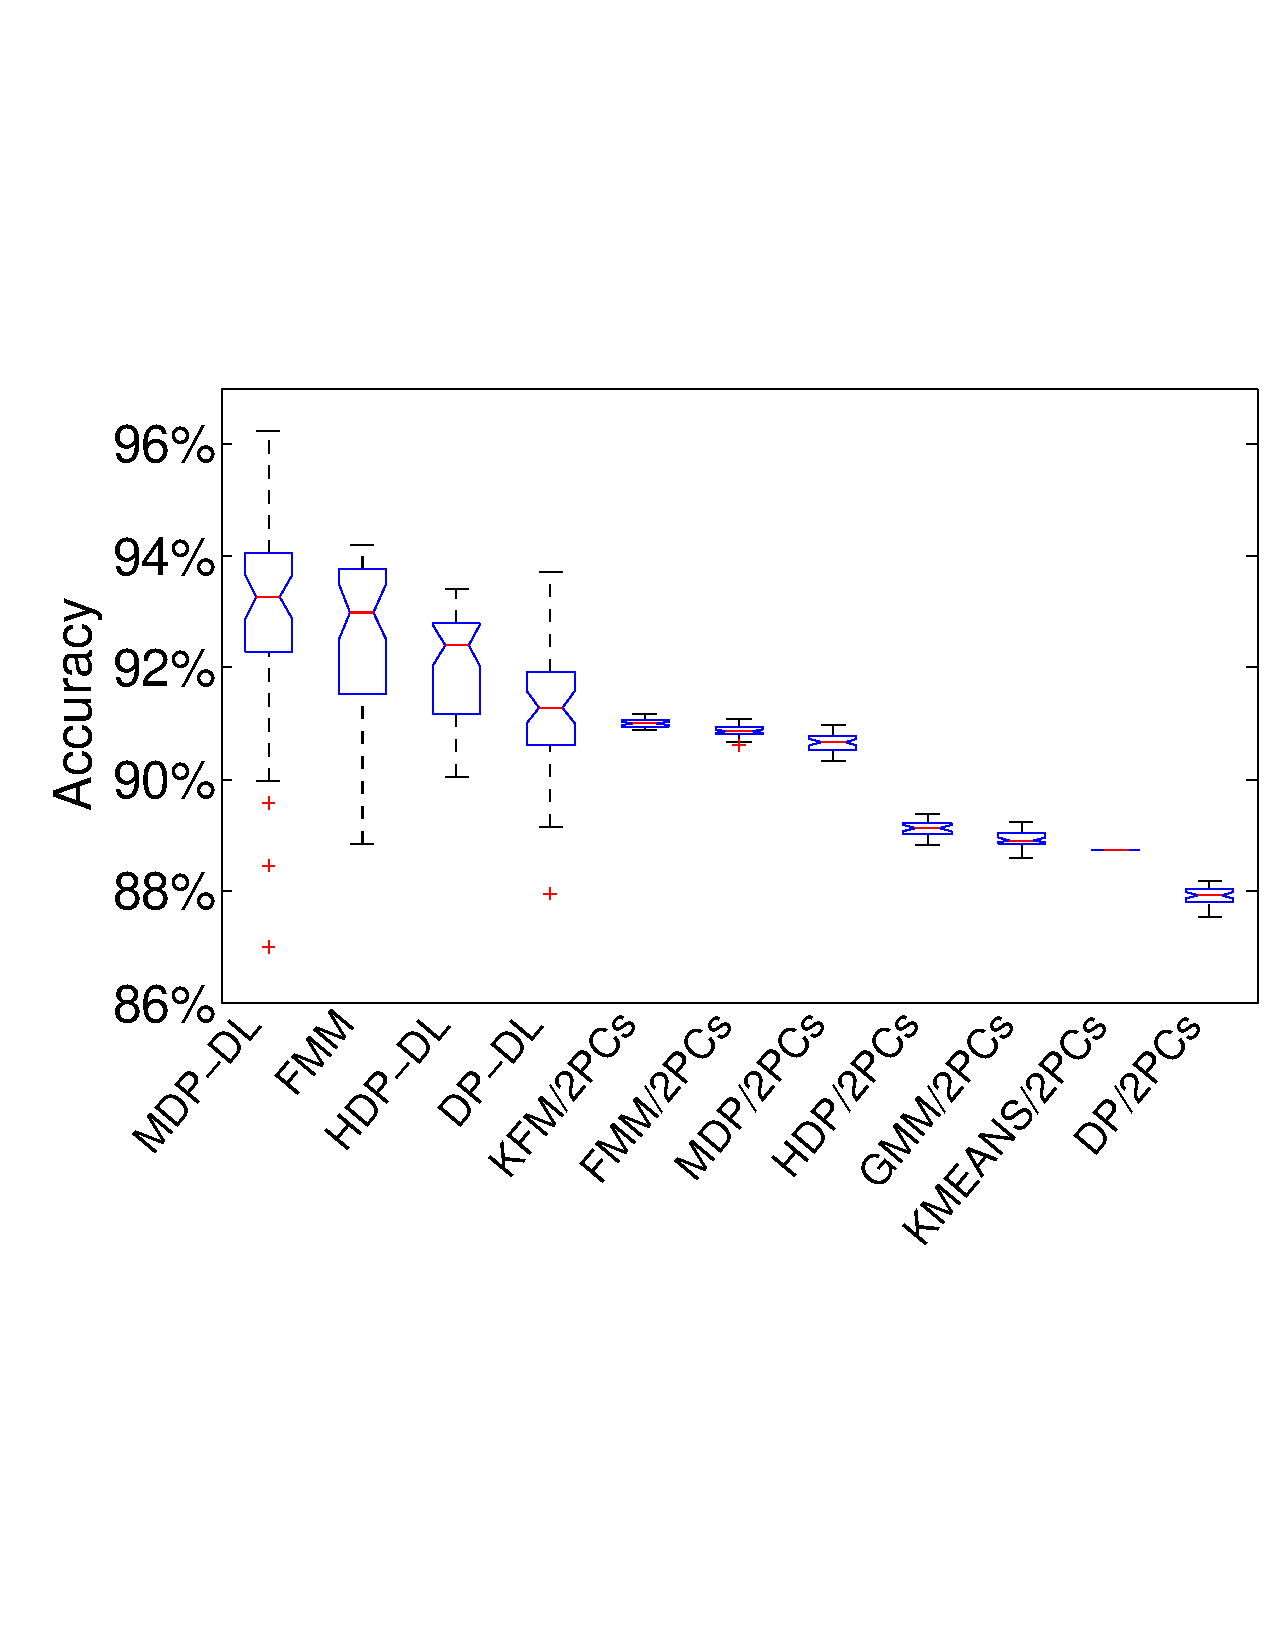
\includegraphics[width=0.48\textwidth]{figs_new/Accuracy_hc_1.pdf}
    \caption{\textit{\small{ Results from testing on d533101 data \cite{Henze2000}. KFM represents Kalman Filter
Mixture method \cite{Calabrese2010}.GMM is Gaussian Mixture method \cite{bishop2006}. 2 PCs denotes using the top 2 principle components, and results were indistinguishable from using the top 3 principle components. For the proposed model, dictionary learning was done as in Sec. \ref{sec:dict}, and ``FMM'' corresponds to the focused mixture-model of Sec. \ref{sec:focused}}}}
\label{fig:Accuracy_hc_1}
\end{figure}

\subsection{Handling missing data}

The quantity of data acquired by a neural recording system is enormous, and therefore in many systems one first performs spike detection ($e.g.$, based on a threshold), and then a signal is extracted about each detection (a temporal window is placed around the peak of a given detection). This step is often imperfect, and significant portions of many of the spikes may be missing due to the windowed signal extraction (and the missing data are not retainable, as the original data are discarded). Conventional feature-extraction methods typically cannot be applied to such temporally clipped signals.

Returning to (\ref{eq:basic}), this implies that some columns of the data $\Xmat_{ij}$ may have missing entries. Conditioned on $\Dmat$, $\Lambdamat$, $\Smat_{ij}$, and $(\eta_1,\dots,\eta_T)$, we have $\Xmat_{ij}\sim\mathcal{N}(\Dmat\Lambdamat\Smat_{ij},\mbox{diag}(\eta_1^{-1},\dots,\eta_T^{-1})$. The missing entries of $\Xmat_{ij}$ may be treated as random variables, and they are integrated out analytically within the Gaussian likelihood function. Therefore, for the case of missing data in $\Xmat_{ij}$, we simply evaluate (\ref{eq:basic}) at the points of $\Xmat_{ij}$ for which data are observed. The columns of the dictionary $\Dmat$ of course have support over the entire signal, and therefore given the inferred $\Smat_{ij}$ (in the presence of missing data), one may impute the missing components of $\Xmat_{ij}$ via $\Dmat\Lambdamat\Smat_{ij}$. As long as, across all $\Xmat_{ij}$, the same part of the signal is not clipped away (lost) for all observed spikes, by jointly processing all of the data (all spikes) we may infer $\Dmat$, and hence infer missing data.

In practice we are less interested in observing the imputed missing parts of $\Xmat_{ij}$ than we are in simply clustering the data, in the presence of missing data. By evaluating $\Xmat_{ij}\sim\mathcal{N}(\Dmat\Lambdamat\Smat_{ij},\mbox{diag}(\eta_1^{-1},\dots,\eta_T^{-1})$ only at points for which data are observed, and via the mixture model in (\ref{eq:mixture}), we directly infer the desired clustering, in the presence of missing data (even if we are not explicitly interested in subsequently examining the imputed values of the missing data).

To examine the ability of the model to perform clustering in the
presence of missing data, we reconsider the publicly available data
from Section \ref{sec:truth}. For the first 10\% of the spike
signals (300 spike waveforms), we impose that a fraction of
the beginning and end of the spike is absent. The original signals
are of length $T=40$ samples. As a demonstration, for the ``clipped'' signals, the first 10 and the last 16 samples of the
signals are missing. A clipped waveform example is shown in Figure \ref{fig:Recovery_waveform}; we compare the mean estimation of the signal, and the error bars reflect one standard deviation from the full posterior on the signal.
In the context of the analysis, we processed all of the data as before, but now with these ``damaged''/clipped signals. We observed that 94.11\% of the non-damaged signals were clustered properly (for the one neuron for which we had truth), and 92.33\% of the damaged signals were sorted properly. The recovered signal in Figure \ref{fig:Recovery_waveform}(a) is typical, and is meant to give a sense of the accuracy of the recovered missing signal. The ability of the model to perform spike sorting in the presence of substantial missing data is a key attribute of the dictionary-learning-based framework.

%Additionally,  we show example of original spike and recovered spike (Figure \ref{fig:Recovery_waveform} and relative recovery errors (Figure \ref{fig:Relative_Error}) for missing data based on the aforementioned dictionary-based imputation.

\begin{figure}[!htbp]
\centering

\subfigure[]{
   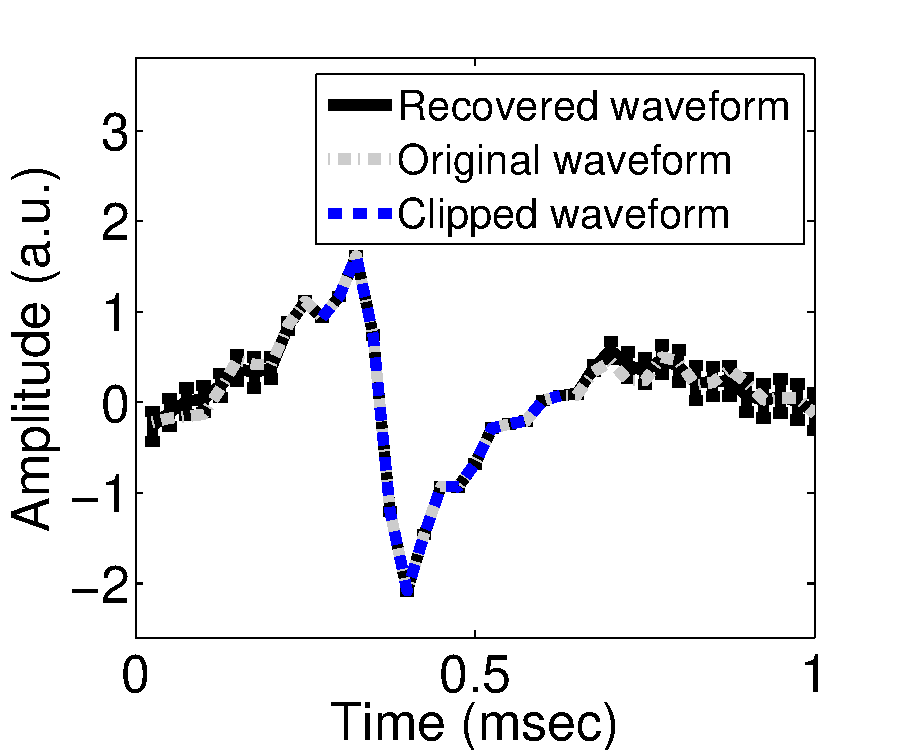
\includegraphics[scale=0.4,angle=0] {figs_new/Recovery_waveform.pdf}
   \label{fig:Recovery_waveform}

 }
 \subfigure[]{
   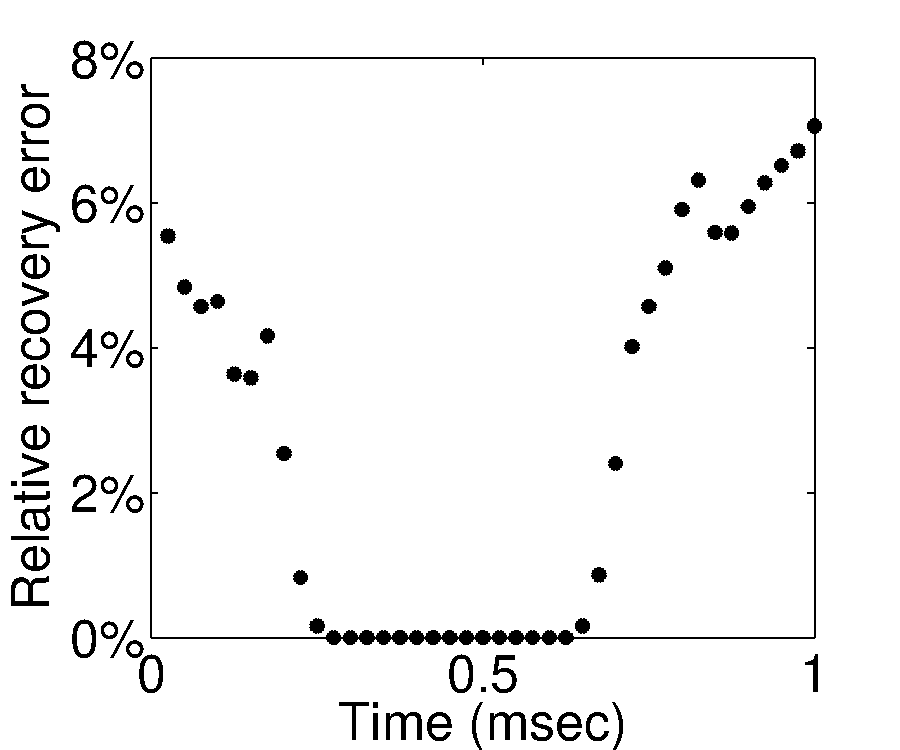
\includegraphics[scale=0.4,angle=90] {figs_new/Relative_recovery_errors.pdf}
   \label{fig:Relative_Error}
 }
  \caption{\small \emph{ (a) Example of a clipped waveform (blue), original waveform (gray) and
  recovery waveform (black); the error bars reflect one standard deviation, from the posterior distribution on the underlying signal. (b) Relative recovery errors (with respect to the mean estimated signal).
   }}
\end{figure}

%A practical example for missing data will be shown. As is known to us that what we get from Plexon software (which is a popular and important analysis software for systems neuroscience research) are unaligned spike waveforms, as shown (Figure \ref{fig:unaligned_waveforms}, however, waveform alignment operation is an important step in the spike sorting. The problem is that part of a spike signal may be clipped off and discarded when the operation is done, Figure \ref{fig:example_missing_waveforms} shows examples of clipped waveforms (red) whose missing samples are more than 10 and  recovery of corresponding waveforms (blue) based on the proposed method.
%
%\begin{figure}[!htbp]
%\centering
%%\subfigure[]{
%%   \includegraphics[scale=0.25,angle=0] {unlignment_waveforms.eps}
%%   \label{fig:unlignment_waveforms}
%% }
% \subfigure[]{
%   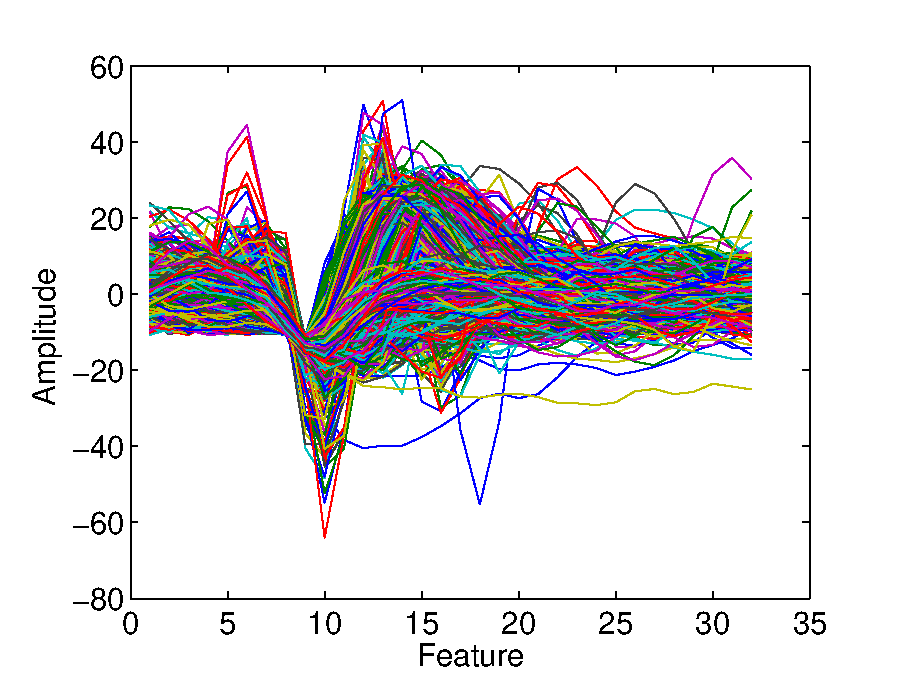
\includegraphics[scale=0.25,angle=0] {unaligned_waveforms.eps}
%   \label{fig:unaligned_waveforms}
%
% }
% \subfigure[]{
%   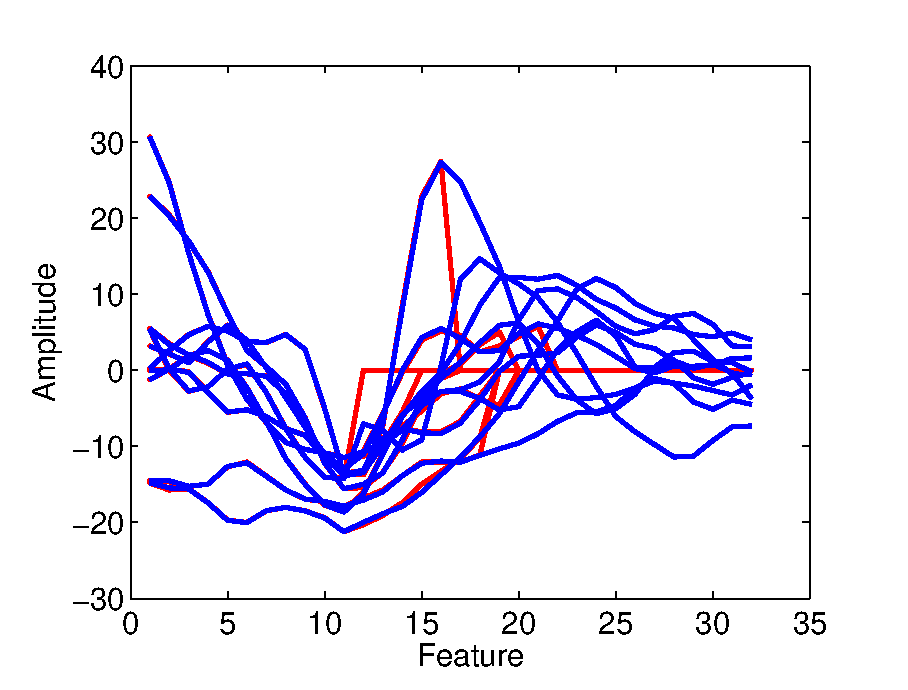
\includegraphics[scale=0.25,angle=0] {example_missing_waveforms.eps}
%   \label{fig:example_missing_waveforms}
% }
%  \caption{\small \emph{(a) Unaligned spike waveforms direct from Plexon software.
% (b) Example of clipped waveforms  (red) and recovery of corresponding waveforms (blue).
%   }}
%\end{figure}


\subsection{Forensic analysis of new longitudinal ephys data\label{sec:forensics}}

The next dataset is new, based upon experiments we have performed with freely moving rats (institutional review board approvals were obtained). These data will be made available to the research community. NeuroNexus$^{\mbox{TM}}$ sensors (Figure \ref{fig:device}) were humanely placed in the motor cortex, and ephys data were measured during one-hour periods on eight consecutive days, starting on the day after implant (data were collected for additional days, but the signal quality degraded after 8 days, as discussed below). Note that nearby sensors are close enough to record the signal of a single or small group of neurons, termed a single-unit event. However, all eight sensors in a line are too far separated to simultaneously record a single-unit event on all eight.

%\begin{table}[t] \caption{\textit{\small{\label{table:HC1} Results from testing on d533101 data \cite{Henze2000}. KFM represent Kalman Filter
%Mixture method \cite{Calabrese2010}. All results, except M-DP and M-FMM with 2 PCs and other two results of the proposed method, are taken from \cite{Bo2011}.  2 PCs denotes using the top 2 principle components, and results were indistinguishable from using the top 3 principle components. For the proposed model, dictionary learning was done as in Sec. \ref{sec:dict}, and ``FMM'' corresponds to the focused mixture-model of Sec. \ref{sec:focused}}}}
%%\begin{center}
%%\begin{tabular}{|c|c|c|c|c|}
%%\hline K-means & GMM & K-means w/ 2 PCs & GMM w/ 2 PCs  & HDP w/ 2 PCs \\
%%\hline
%%88.08\% & 87.42\% &  88.44\% & 89.04\%  & 89.54 \\
%%\hline
%%\end{tabular}
%%\begin{tabular}{|c|c|c|c|}
%%\hline DP-DL & HDP-DL &  M-DP w/ 2 PCs  & Proposed DP-DL \\
%%\hline
%%  91.89\% & 93.05\% & 91.21\% & 94.4\% \\
%%\hline
%%\end{tabular}
%%\begin{tabular}{|c|c|c|c|}
%%\hline KFM w/ 2 PCs & DP w/ 2 PCs & M-FMM w/ 2 PCs & Proposed FMM\\
%%\hline
%% 88.36\% & 88.07\% & 91.21\%  & 93.7\%\\
%%\hline
%%\end{tabular}\end{center}
%%\end{table}
%
%
%
%\begin{center}
%\begin{tabular}{|c|c|c|c|}
%\hline K-means & GMM & K-means w/ 2 PCs & GMM w/ 2 PCs   \\
%\hline
%88.08\% & 87.42\% &  88.44\% & 89.04\%   \\
%\hline
%\end{tabular}
%\begin{tabular}{|c|c|c|}
%\hline  DP w/ 2 PCs & HDP w/ 2 PCs & KFM w/ 2 PCs    \\
%\hline
%     88.07\% & 89.54\% & 88.36\% \\
%\hline
%\end{tabular}
%\begin{tabular}{|c|c|c|}
%\hline  M-DP w/ 2 PCs &  M-FMM w/ 2 PCs & DP-DL    \\
%\hline
%      91.21\%  & 91.21\% & 91.89\% \\
%\hline
%\end{tabular}
%\begin{tabular}{|c|c|c|}
%\hline  HDP-DL &  Proposed DP-DL &  Proposed FMM\\
%\hline
%  93.05\% & 94.4\%  & 93.7\%\\
%\hline
%\end{tabular}
%\end{center}
%\end{table}



The data were bandpass filtered (0.3-3 kHz), and
then all signals 3.5 times the standard deviation of the background
signal were deemed detections. The peak of the detection was placed
in the center of a 1.3 msec window, which corresponds to $T=40$
samples at the recording rate. The signal
$\Xmat_{ij}\in\mathbb{R}^{T\times N}$ corresponds to the data
measured simultaneously across all $N$ channels within this window.
Here $N=8$, with a concentration on the data measured from the 8
channels of the zoomed-in Figure \ref{fig:device}.

%begin{figure}[ht]\vspace{-5mm}
% \centering
%\subfigure[1]{
%\includegraphics[scale=0.3]{device.eps} %height=3.5cm, width=4.5cm,angle=0
%\label{fig:device}}
% \subfigure[2]{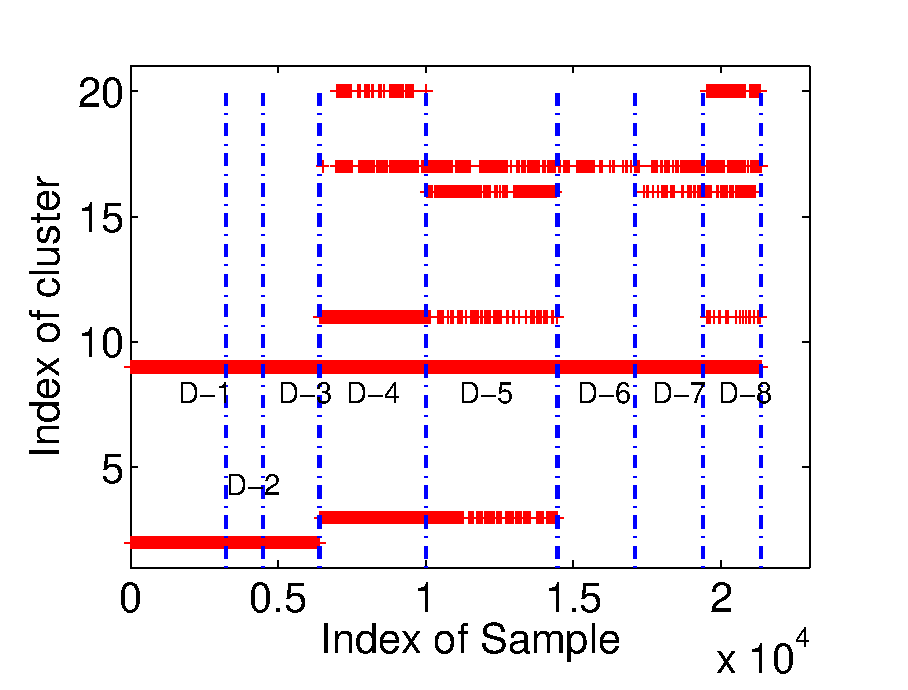
\includegraphics[scale=0.3]{clustering.eps}
%\label{fig:global_clustering}}
% \subfigure[3]{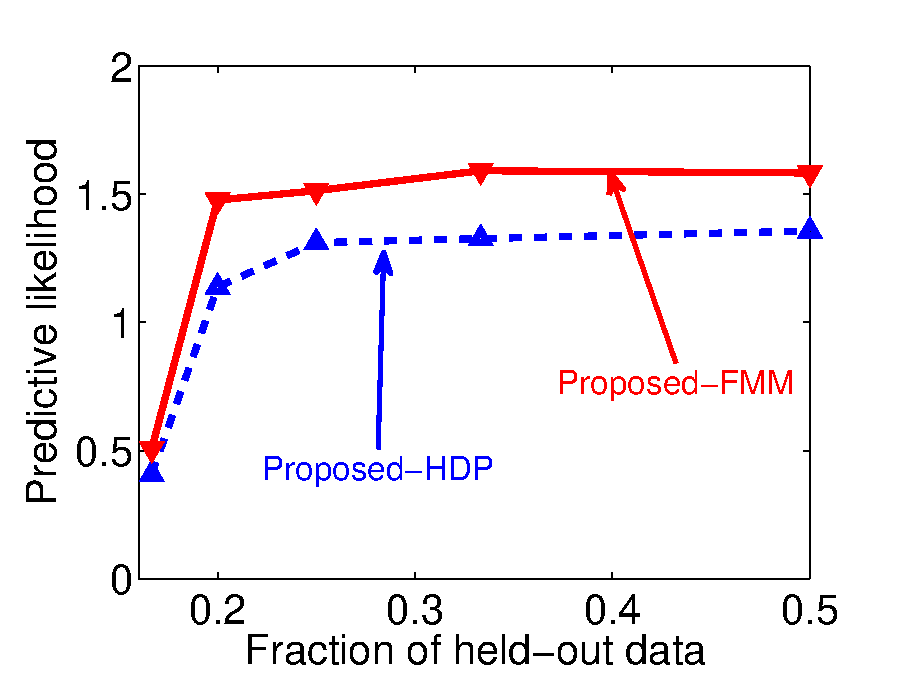
\includegraphics[scale=0.3]{likelihood.eps}
%\label{fig:likelihood}} \vspace{-5mm} \caption{ \small \emph{(a)
%Schematic of the neural recording array that was placed in the rat
%motor cortex. The red numbers identify the sensors, and a zoom-in of
%the bottom-eight sensors is shown. The sensors are ordered by the
%order of the read-out pads, at left. (b) From the maximum-likelihood
%collection sample, the apportionment of data among mixture
%components (clusters). Results are shown for 45 sec recording
%periods, on each of 8 days. (c) Predictive likelihood of held-out
%data. The horizontal axis represents the fraction of data used for
%model training.}}
%\end{figure}

\begin{figure}[!htbp]
\centering

\subfigure[]{
   \includegraphics[scale=0.20,angle=0] {figs_new/device.eps}
   \label{fig:device}

 }
 \subfigure[]{
   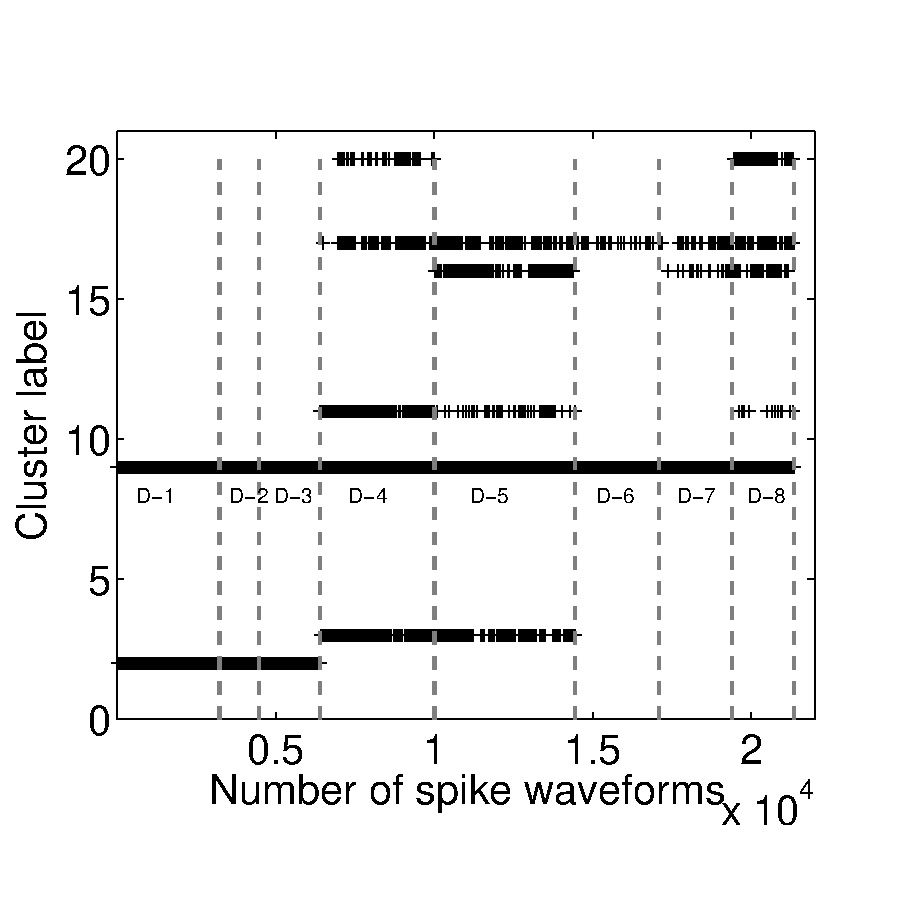
\includegraphics[scale=0.4,angle=0] {figs_new/clustering.pdf}
   \label{fig:glob_clustering}
 }
 \subfigure[]{
   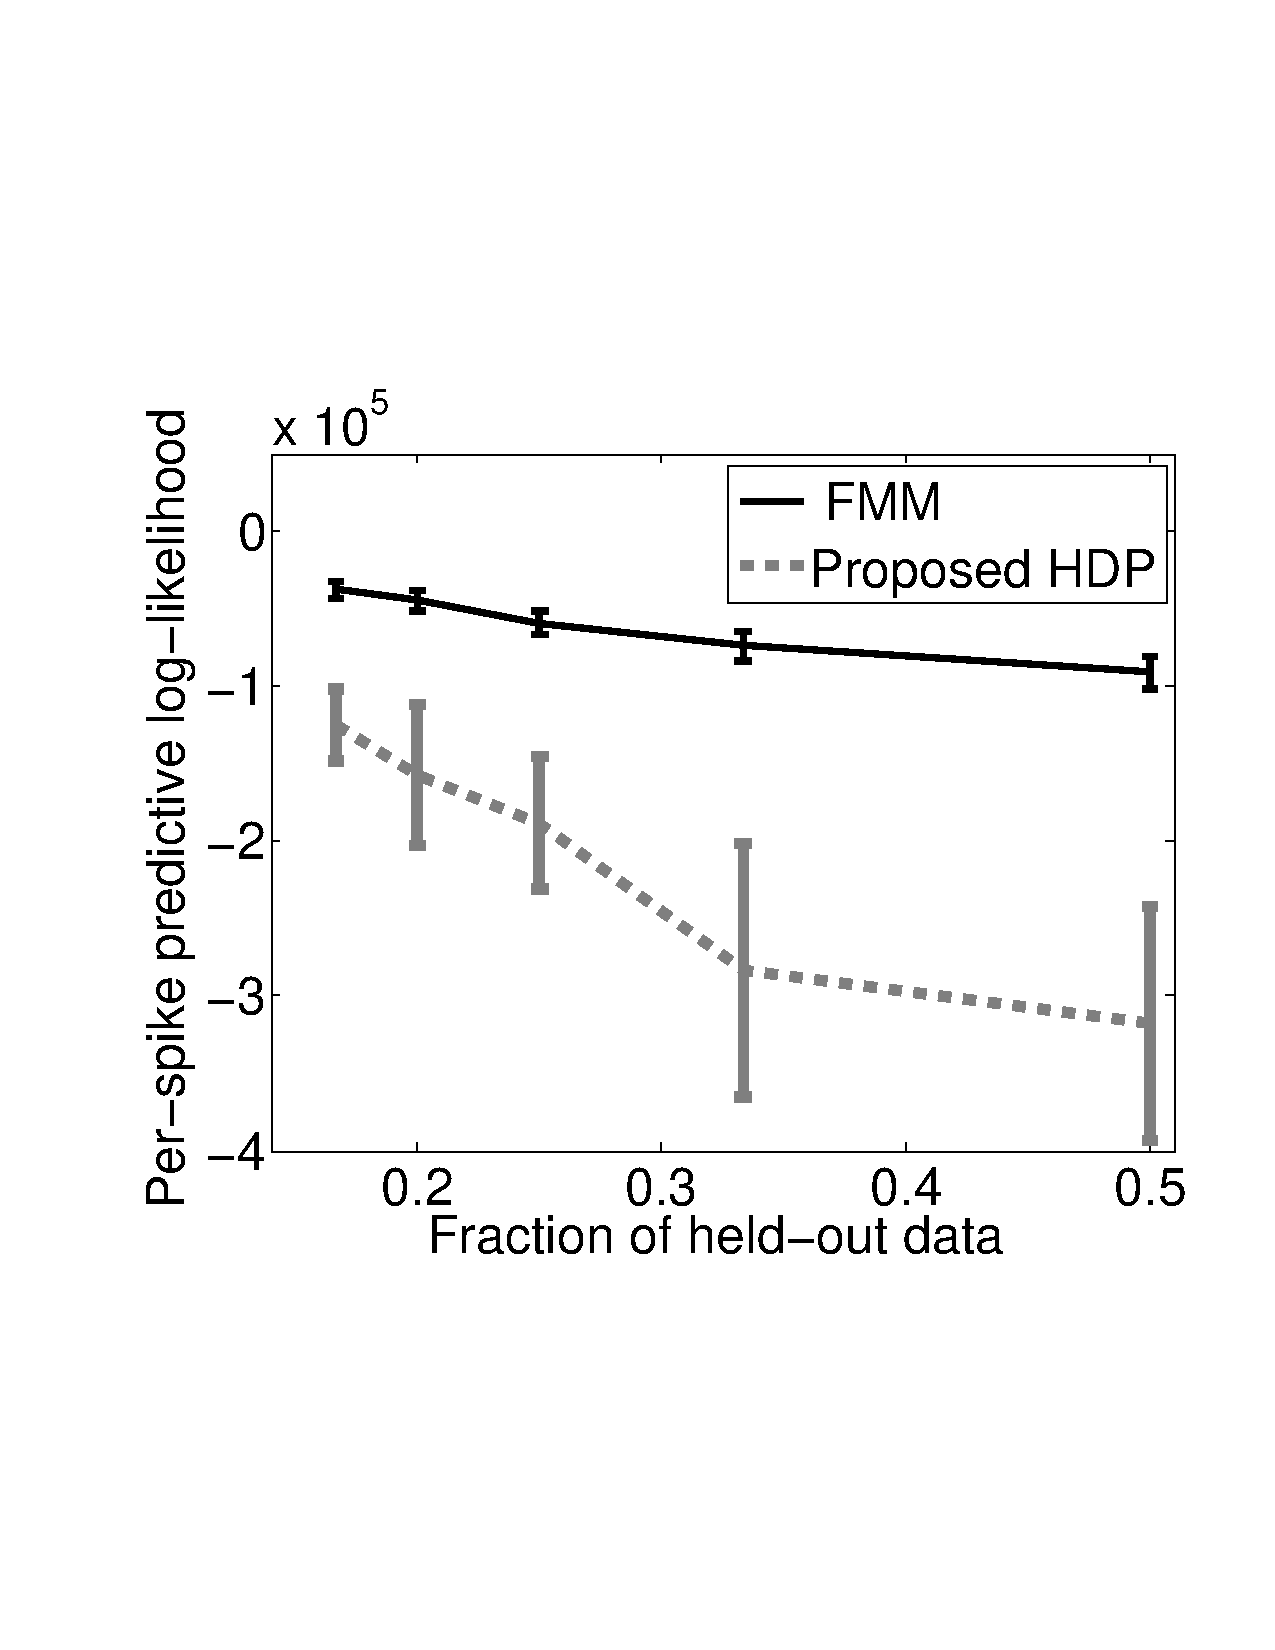
\includegraphics[scale=0.4,angle=0] {figs_new/likelihood2.pdf}
   \label{fig:likelihood}
 }
  \caption{\small \emph{(a) Schematic of the neural
recording array that was placed in the rat motor cortex. The red
numbers identify the sensors, and a zoom-in of the bottom-eight
sensors is shown. The sensors are ordered by the order of the
read-out pads, at left. The presented data are for sensors numbered 1 to 8, corresponding to the zoomed-in region. (b) From the maximum-likelihood collection
sample, the apportionment of data among mixture components
(clusters). Results are shown for 45 sec recording periods, on each
of 8 days. For example, D-4 reflects data on day 4. Note that while the truncation level is such that there are 20 candidate clusters (vertical axis in (b)), only an inferred subset of clusters are actually used. (c) Predictive likelihood of held-out data. The
horizontal axis represents the fraction of data held out during training.}}
\end{figure}

In Figure \ref{fig:glob_clustering} are shown assignments of data to each of the possible clusters, for data measured across the 8 days, as computed by the proposed model ($e.g.$, for the first three days, two clusters were inferred). Results are shown for the maximum-likelihood collection sample. As a comparison to the proposed focused mixture model (FMM) of Section \ref{sec:focused}, we also considered the simplified HDP construction discussed in Section \ref{sec:related}, with the $\bv^{(i)}$ set to all ones (in both cases we employ the same form of dictionary learning, as in Section \ref{sec:dict}). From Figure \ref{fig:likelihood}, it is observed that on held-out data the FMM yields improved results relative to the traditional HDP.

In fact, the proposed model was developed specifically to address the problem of multi-day forensic analysis of ephys data, as a consequence of observed limitations of HDP (which are only partially illuminated by Figure \ref{fig:likelihood}). Specifically, while the focused nature of the FMM allows learning of specialized clusters that occur over limited days, the ``non-focused'' HDP tends to merge similar but distinct clusters. This yields HDP results that are characterized by fewer total clusters, and by cluster characteristics that are less revealing of detailed neural processes. Patterns of observed neural activity may shift over a period of days due to many reasons, including cell death, tissue encapsulation, or device movement; this shift necessitates the FMM's ability to focus on subtle but important differences in the data properties over days. This ability to infer subtly different clusters is related to the focused topic model's ability  \cite{compound} to discern distinct topics that differ in subtle ways. The study of large quantities of data (8 days) makes the ability to distinguish subtle differences in clusters more challenging (the DP-DL-based model works well when observing data from one recording session, like in Figure \ref{fig:Accuracy_hc_1}, but the analysis of multiple days of data is challenging for HDP).



%\begin{figure}[!htbp]\vspace{-12.5mm}
% \centering
%
%\subfigure[]{
%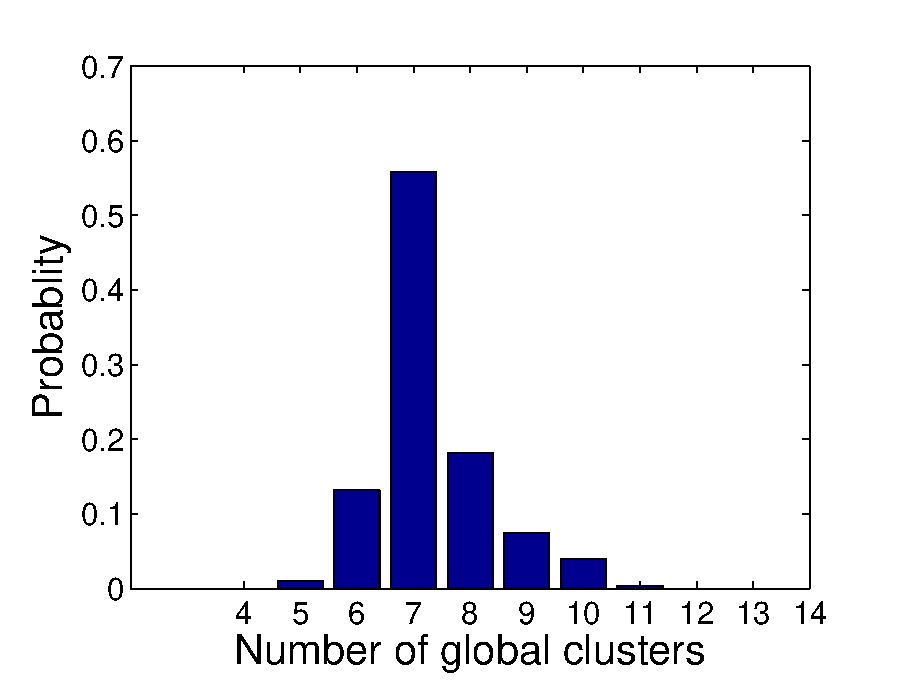
\includegraphics[height=3cm, width=4cm,angle=0]{posterior_a.eps}
%\label{fig:post_clusters}}
% \subfigure[]{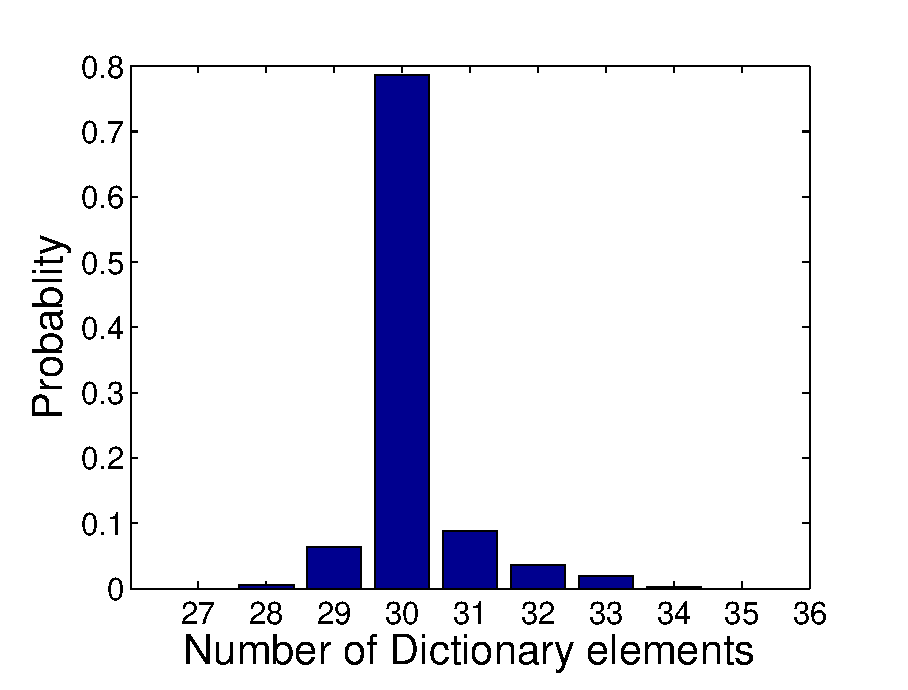
\includegraphics[height=3cm, width=4cm,angle=0]{posterior_b.eps}
%\label{fig:post_dict}}
% \subfigure[]{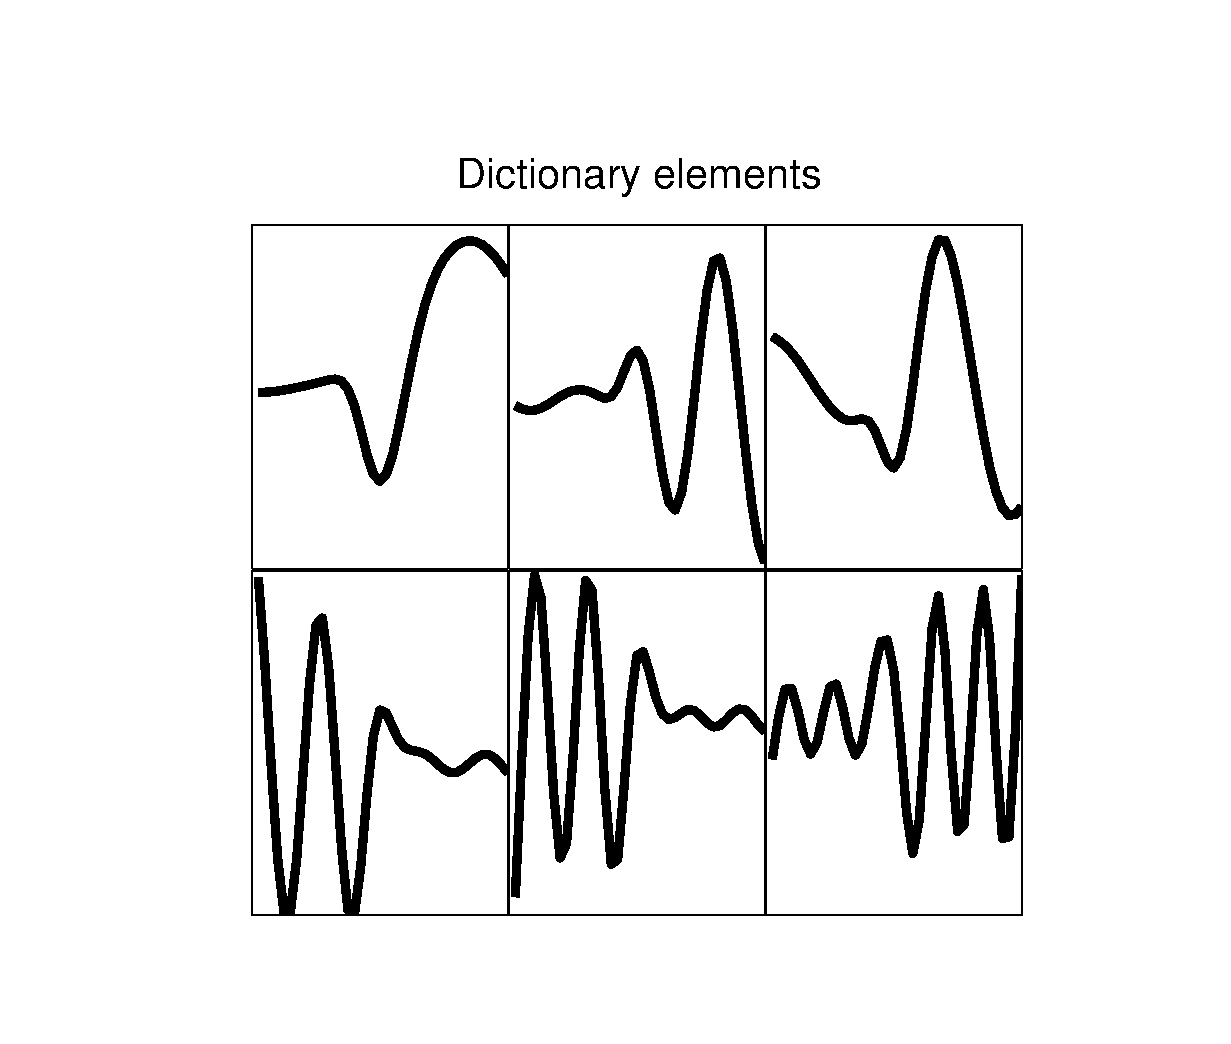
\includegraphics[height=3cm, width=4cm,angle=0]{posterior_c.eps}
%\label{fig:dict_examples}} \vspace{-5mm} \caption{ \small \emph{(a)
%Approximate posterior distribution on the number of global clusters
%(mixture components). (b) Approximate posterior distribution on the
%number of required dictionary elements. (c) Example inferred
%dictionary elements.}}
%\end{figure}



\begin{figure}[!htbp]
\centering

\subfigure[]{
   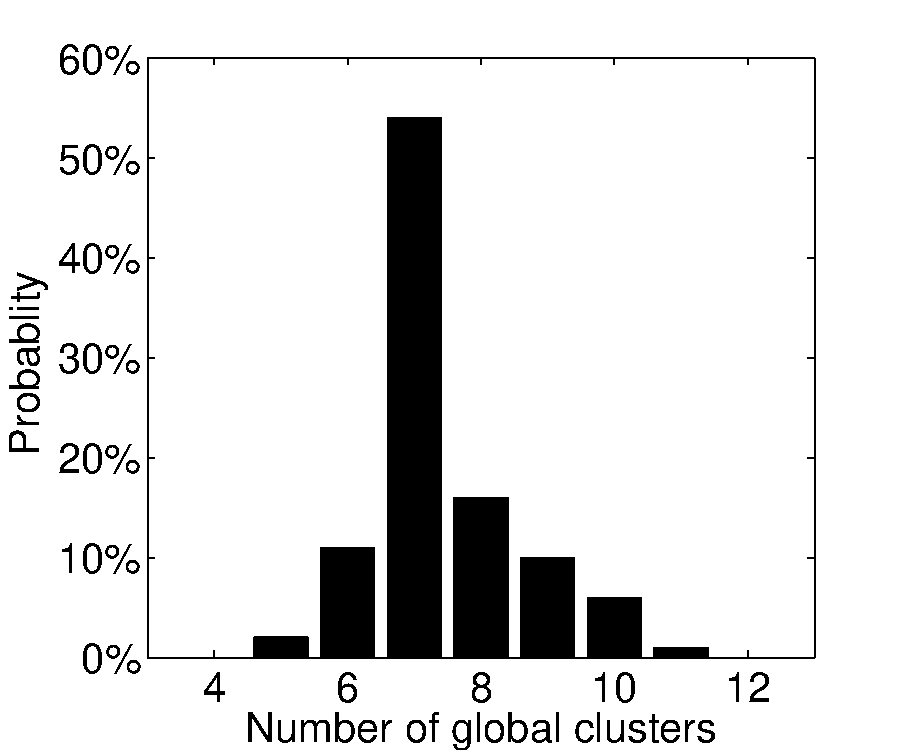
\includegraphics[scale=.4,angle=0] {figs_new/posterior_a.pdf}
   \label{fig:post_clusters}

 }
 \subfigure[]{
   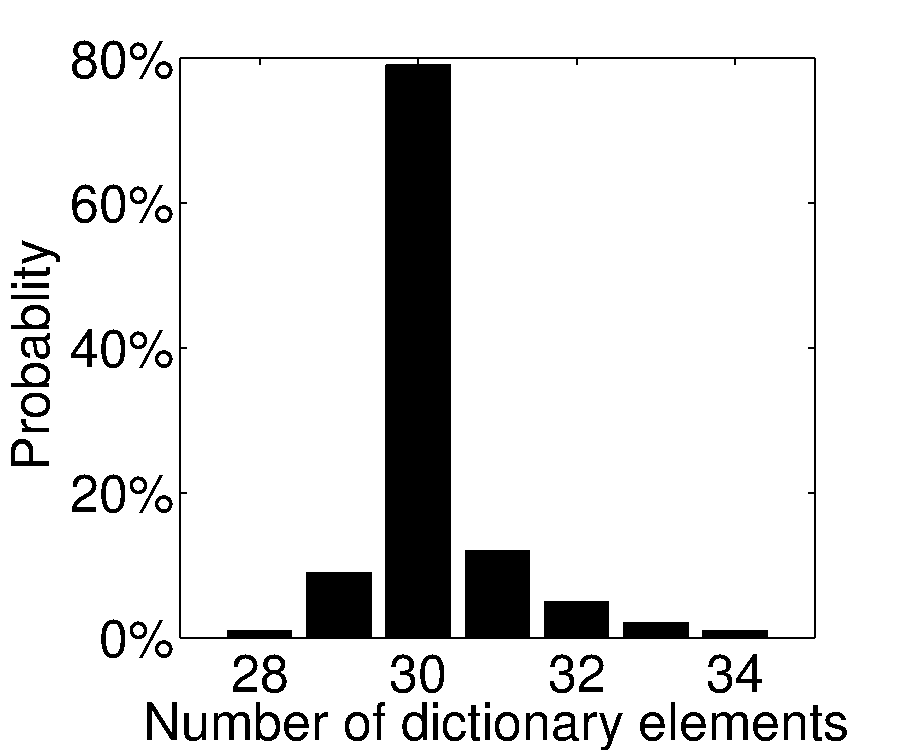
\includegraphics[scale=.4,angle=0] {figs_new/posterior_b.pdf}
   \label{fig:post_dict}
 }\hspace{-3mm}
 \subfigure[]{
   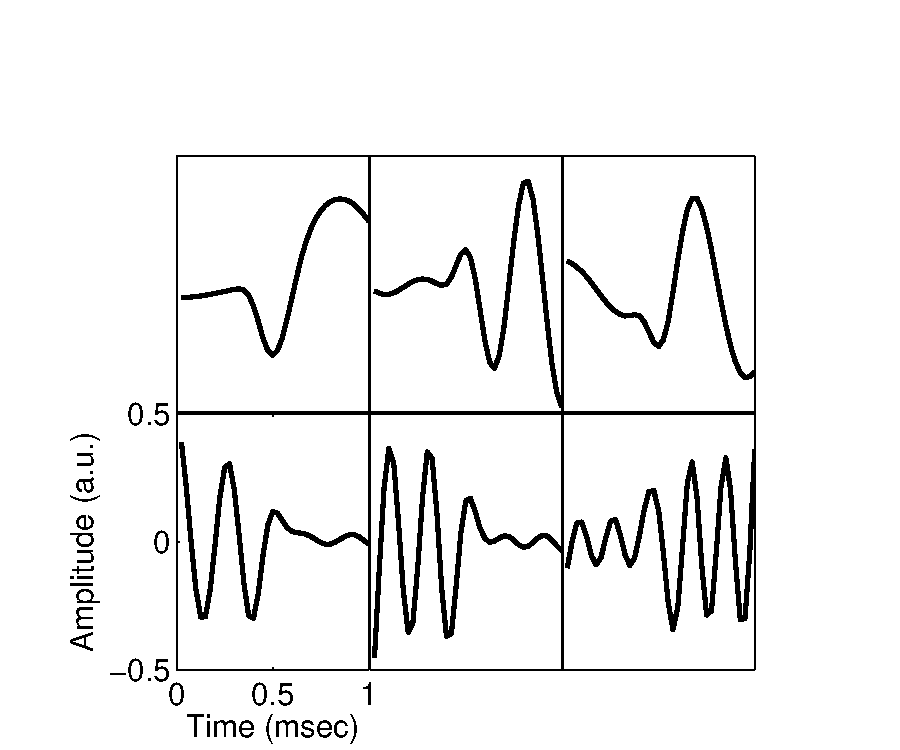
\includegraphics[scale=.5,angle=0] {figs_new/Dictionary_elements.pdf}
   \label{fig:dict_examples}
 }
  \caption{\small \emph{(a) Approximate posterior distribution on the number of global clusters
(mixture components). (b) Approximate posterior distribution on the
number of required dictionary elements. (c) Example inferred
dictionary elements, the unit of amplitude is unitless.}}
\end{figure}


Note from Figure \ref{fig:glob_clustering} that the number of
detected signals is different for different recording days, despite
the fact that the recording period reflective of these data (45
secs) is the same for all days. This highlights the need to allow
modeling of different signal rates, as in our model but not
emphasized in these results.

Among the parameters inferred by the model are approximate posterior
distributions on the number of clusters across all days, and on the
required number of dictionary elements. These approximate posteriors
are shown in Figures \ref{fig:post_clusters}-\ref{fig:post_dict},
and in Figure \ref{fig:dict_examples} are shown example dictionary
elements. Although not shown for brevity, the $\{p_i\}$ had posterior means in excess of 0.9 .

%\begin{figure}[!htbp]
% \centering
%% \subfigure[]{\includegraphics[scale=0.3,angle=0]{figs/intensity_summary.pdf}
%%\label{fig:d561102intra}}
%\subfigure[]{
%\includegraphics[scale=0.25,angle=0]{figs/rat_high_intensity.pdf}
%\label{fig:high}}
% \subfigure[]{\includegraphics[scale=0.25,angle=0]{figs/rat_low_intensity.pdf}
%\label{fig:low}}
%%\subfigure[]{
%%\includegraphics[scale=0.6,angle=0]{figs/global1.pdf}
%%\label{fig:d561102tables}}
%%\hspace{15mm}
%% \subfigure[]{\includegraphics[scale=0.6,angle=0]{figs/global2.pdf}
%%\label{fig:d561102intra}}
%\vspace{-5mm}
%\caption{
%\small \label{fig:video}Examples of high-activity (a), and low-activity (b) recording periods.}
%\end{figure}


To better represent insight that is garnered from the model, in Figure \ref{fig:units} are depicted the inferred properties of three of the clusters, from Day 4 (D-4 in Figure \ref{fig:glob_clustering}). Shown are the \emph{mean} signal for the 8 channels in the respective cluster (for the 8 channels at the bottom of Figure \ref{fig:device}), and the error bars represent one standard deviation, as defined by the estimated posterior. Note that the cluster in Figure \ref{fig:units}(a) corresponds to a localized single-unit event, presumably from a neuron (or a coordinated small group of neurons) near the sensors associated with channels 7 and 8. The cluster in Figure \ref{fig:units}(b) similarly corresponds to a single-unit event situated near the sensors associated with channels 3 and 6. Note the proximity of sensors 7 and 8, and sensors 3 and 6, from Figure \ref{fig:device}. The HDP model uncovered the cluster in Figure \ref{fig:units}(a), but not that in Figure \ref{fig:units}(b).

Note Figure \ref{fig:units}(c), in which the mean signal across all 8 channels is approximately the same (HDP also found related clusters of this type). This cluster is deemed to \emph{not} be associated with a single-unit event, as the sensors are too physically distant across the array for the signal to be observed simultaneously on all sensors from a single neuron. This class of signals is deemed associated with an artifact or some global phenomena, due to (possibly) movement of the device within the brain, and/or because of charges that build up in the device and manifest signals with animal motion. Note that in Figures \ref{fig:units}(a)-\ref{fig:units}(b) the error bars are relatively tight with respect to the strong signals in the set of eight, while the error bars in Figure \ref{fig:units}(c) are more pronounced (the mean curves look clean, but this is based upon averaging thousands of signals).
%
%\begin{figure}[!htbp]
% \centering
%\subfigure[]{
%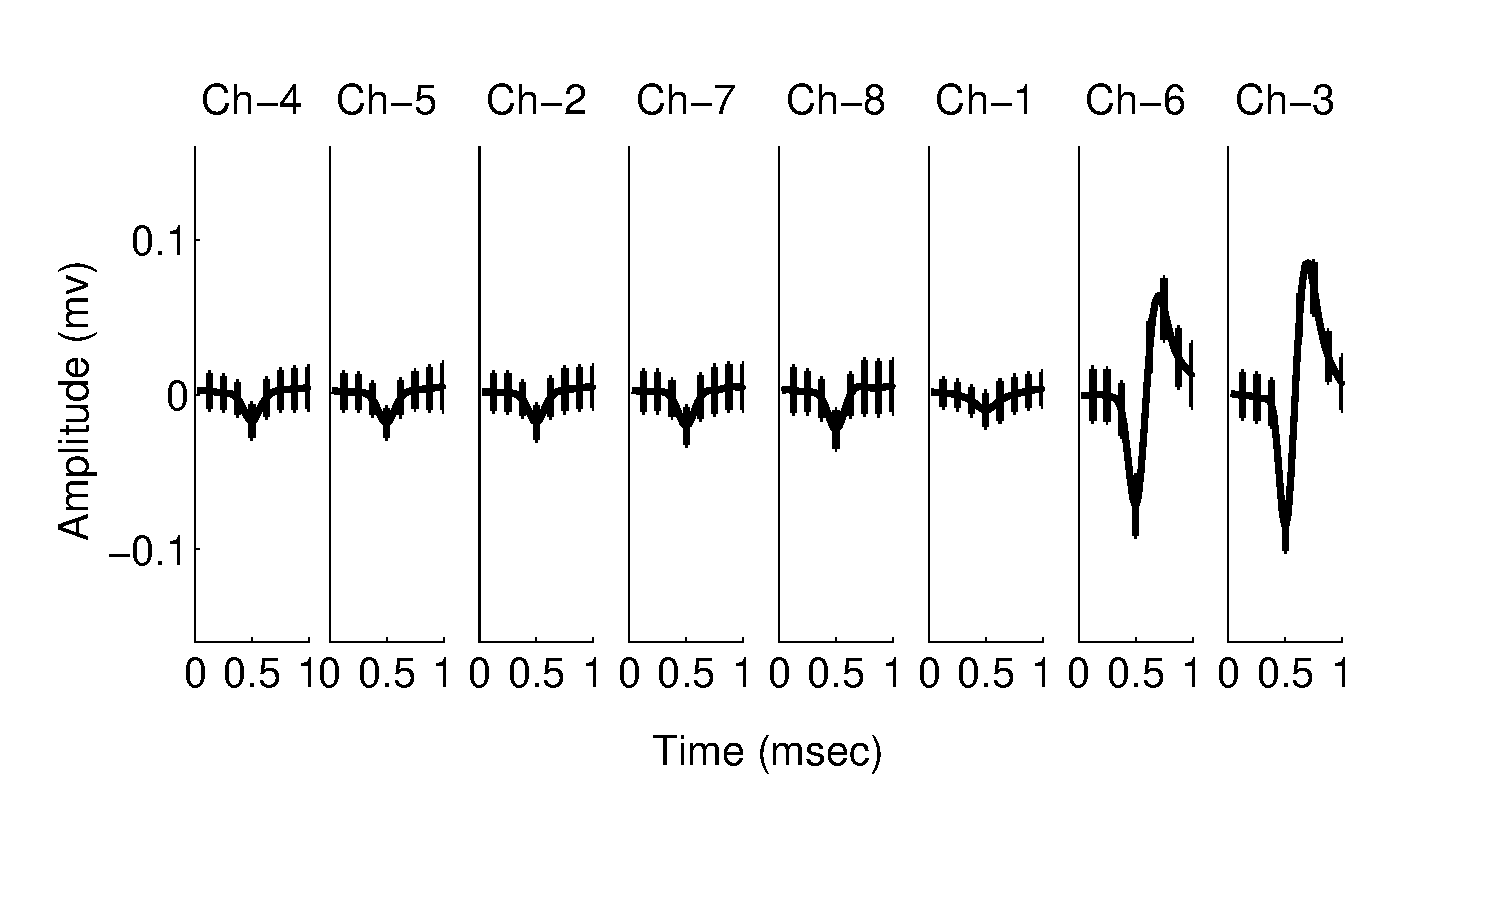
\includegraphics[width=0.48\textwidth]{figs_new/single_event1.pdf}
%\label{fig:single_unit1}}
%\subfigure[]{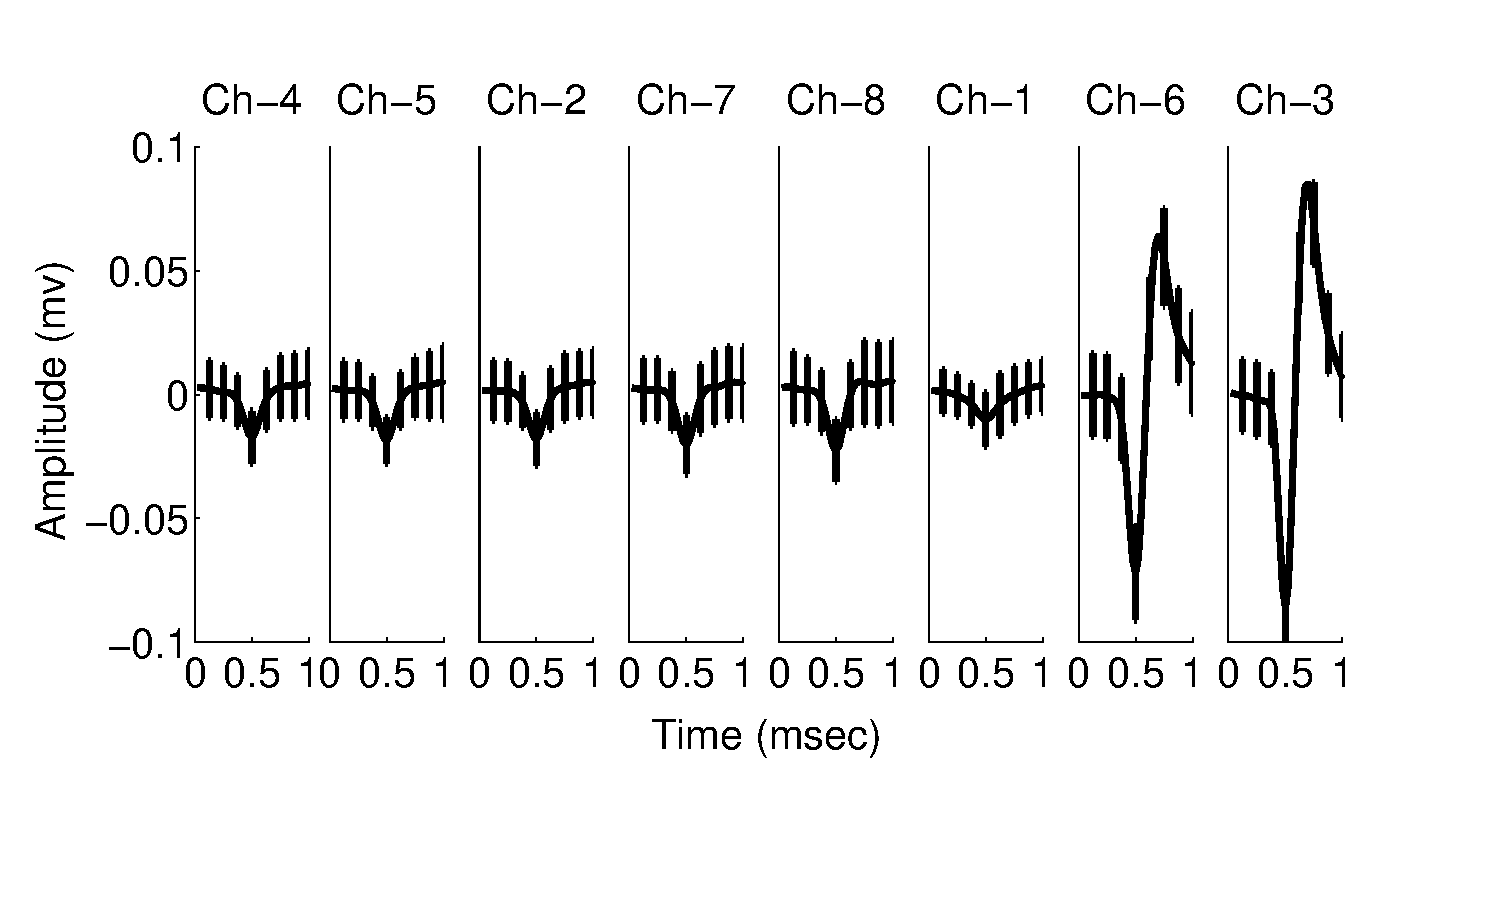
\includegraphics[width=0.48\textwidth]{figs_new/single_event2.pdf}
%\label{fig:single_unit2}} \subfigure[]{
%\includegraphics[width=0.48\textwidth]{figs_new/global1.pdf}
%\label{fig:non_single_unit}}
%% \subfigure[]{\includegraphics[scale=0.6,angle=0]{figs/global2.eps}
%%\label{fig:non_single_unit}}
%\caption{\label{fig:units}\small{\emph{Example
%clusters inferred for data on the bottom 8 channels of Fig.
%\ref{fig:device}. (a)-(b) Example of single-unit events. (c) Example
%of a cluster \emph{not} attributed to a single-unit-event. The 8
%signals are ordered from left to right consistent with the numbering
%of the 8 channels at the bottom of Figure \ref{fig:device}. The blue curves represent the mean, and the error bars are one standard deviation.}}}
%\end{figure}


%\begin{figure}[!htbp]
% \centering
%\subfigure[]{
%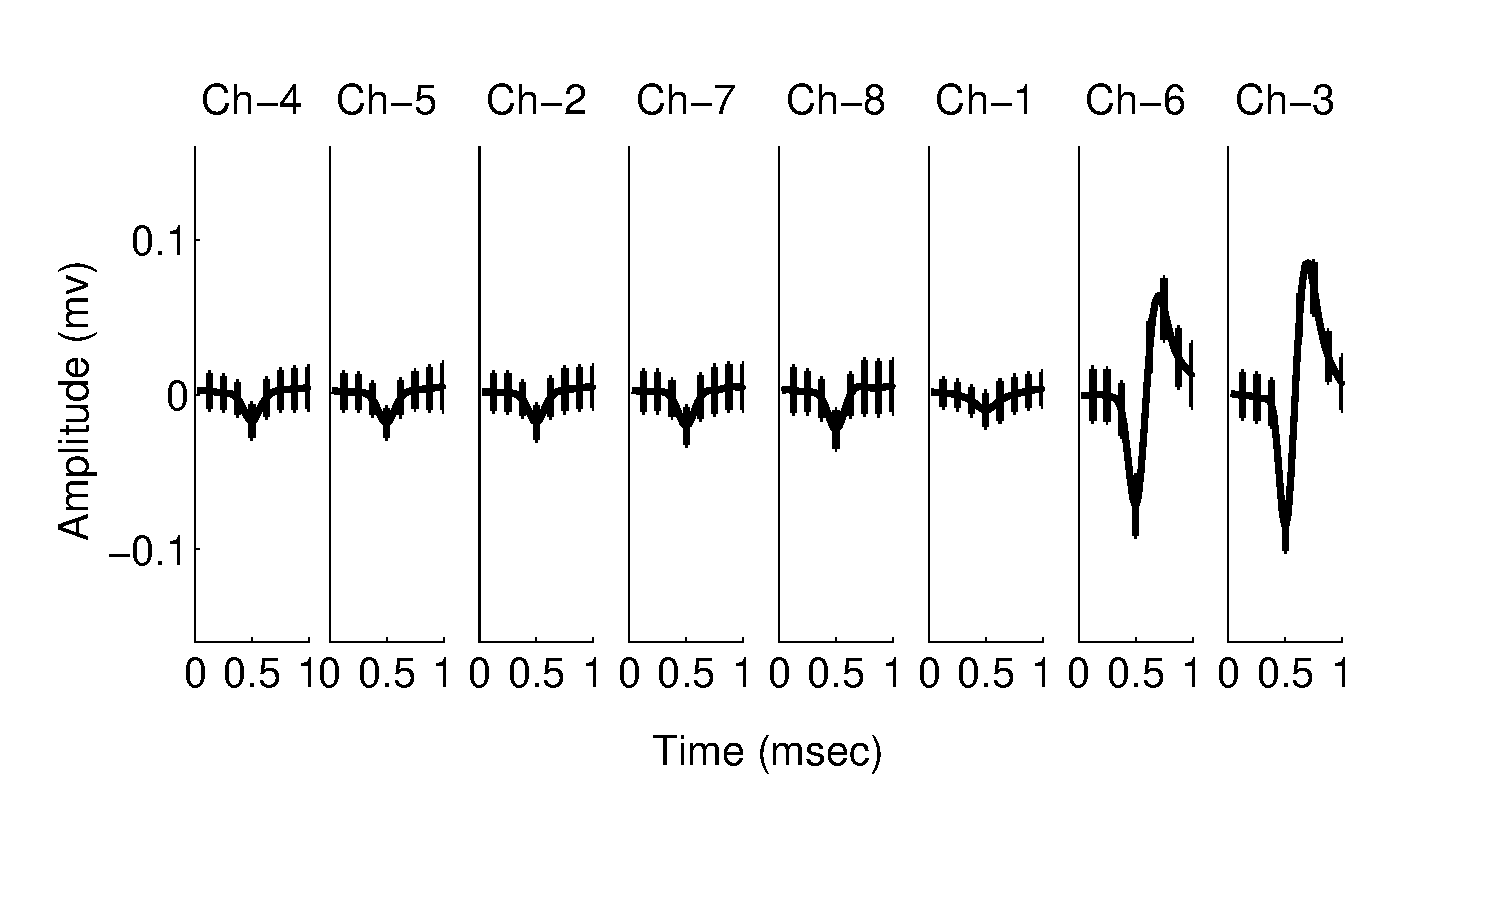
\includegraphics[width=0.48\textwidth]{figs_new/single_event1.pdf}
%\label{fig:single_unit1}}
%\subfigure[]{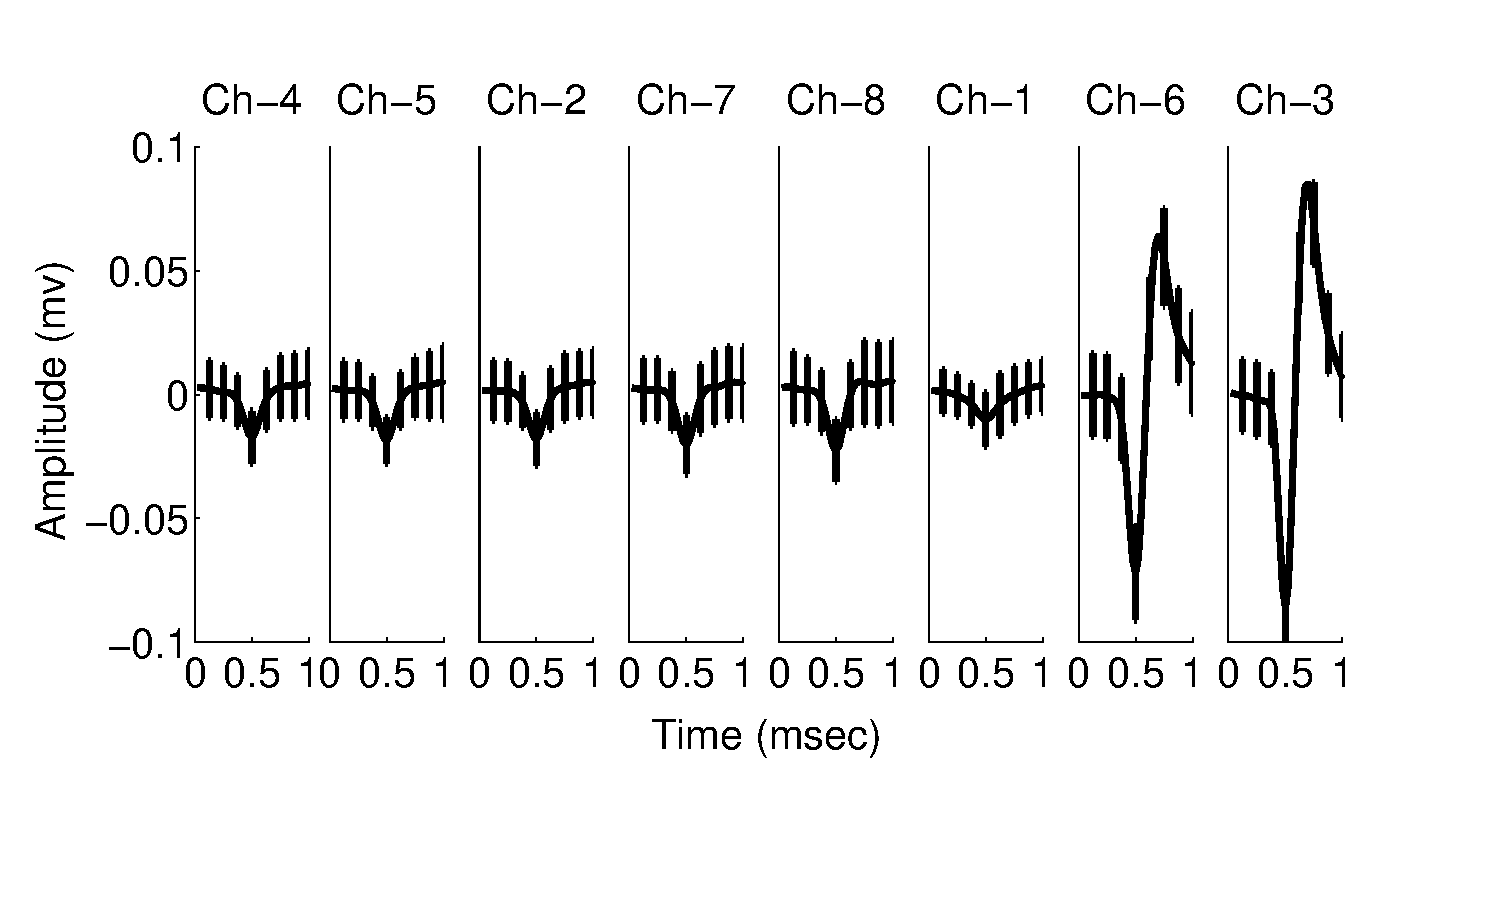
\includegraphics[width=0.48\textwidth]{figs_new/single_event2.pdf}
%\label{fig:single_unit2}} \subfigure[]{
%\includegraphics[width=0.48\textwidth]{figs_new/global1.pdf}
%\label{fig:non_single_unit}}
%% \subfigure[]{\includegraphics[scale=0.6,angle=0]{figs/global2.eps}
%%\label{fig:non_single_unit}}
%\caption{\label{fig:units}\small{\emph{Example
%clusters inferred for data on the bottom 8 channels of Fig.
%\ref{fig:device}. (a)-(b) Example of single-unit events. (c) Example
%of a cluster \emph{not} attributed to a single-unit-event. The 8
%signals are ordered from left to right consistent with the numbering
%of the 8 channels at the bottom of Figure \ref{fig:device}. The blue curves represent the mean, and the error bars are one standard deviation.}}}
%\end{figure}

\begin{figure}[h!]
  \centering
    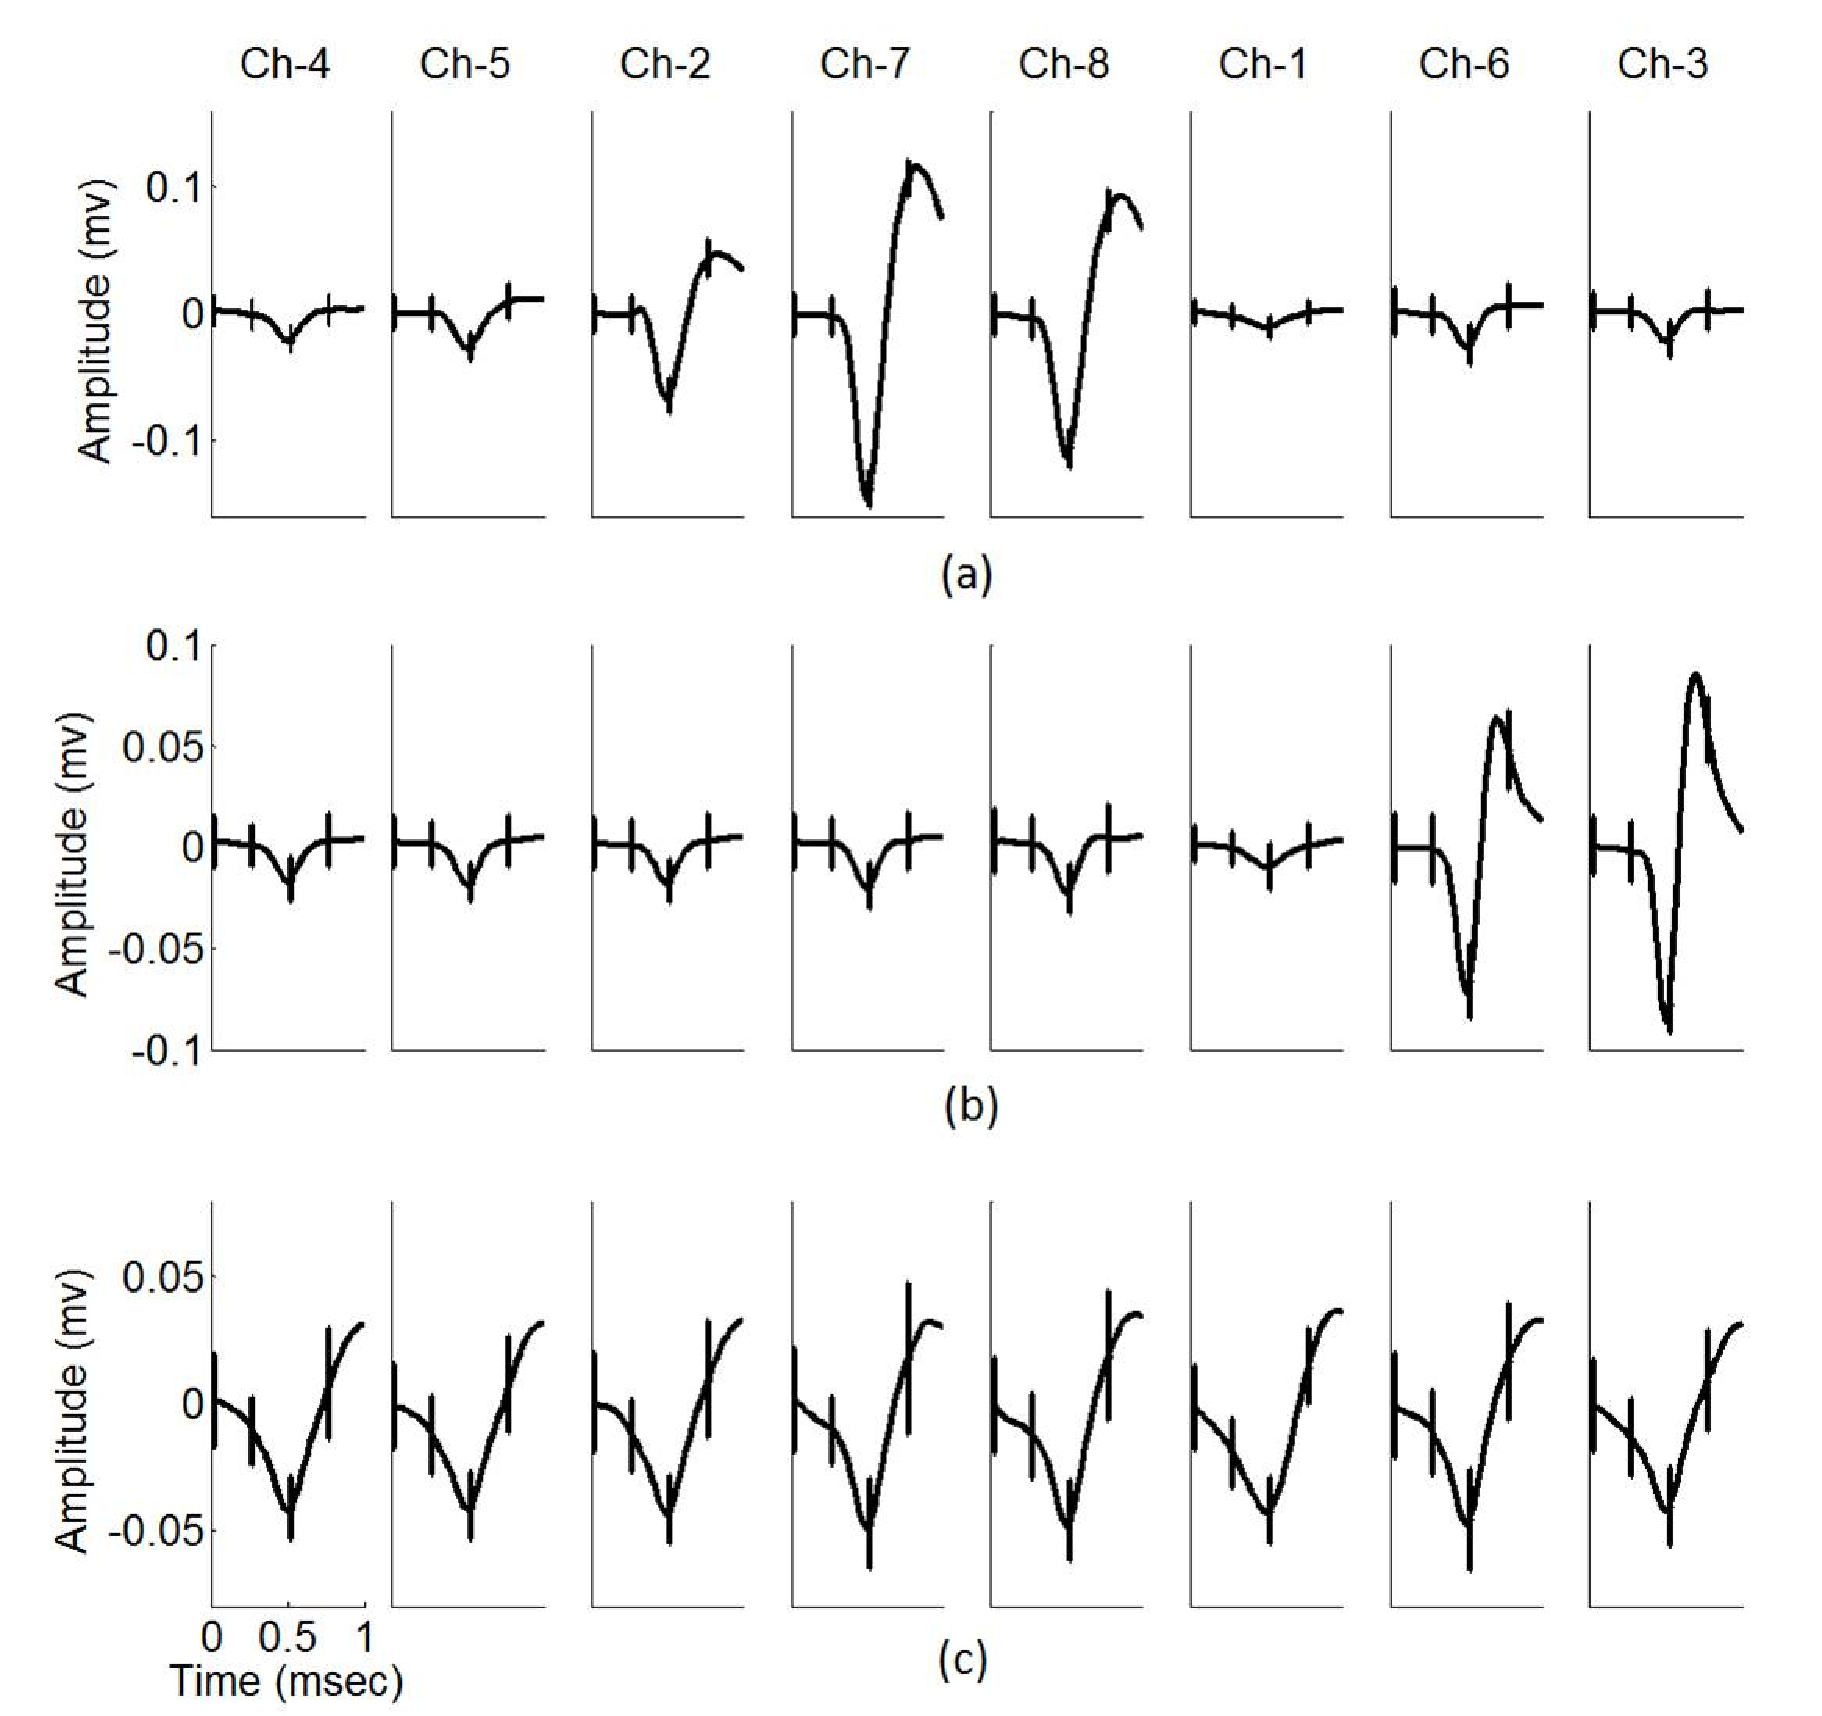
\includegraphics[width=0.48\textwidth]{figs_new/singleunits.pdf}
\caption{\label{fig:units}\small{\emph{Example
clusters inferred for data on the bottom 8 channels of Fig.
\ref{fig:device}. (a)-(b) Example of single-unit events. (c) Example
of a cluster \emph{not} attributed to a single-unit-event. The 8
signals are ordered from left to right consistent with the numbering
of the 8 channels at the bottom of Figure \ref{fig:device}. The blue curves represent the mean, and the error bars are one standard deviation.}}}
\label{fig:units}
\end{figure}
In addition to recording the ephys data, video was recorded of the rat throughout. Robust PCA \cite{Wright09} was used to quantify the change in the video from frame-to-frame, with high change associated with large motion by the animal (this automation is required because one hour of data are collected on each day; direct human viewing is tedious and unnecessary). On Day 4, the model infers that in periods of high animal activity, 20\% to 40\% of the detected signals are due to single-unit events (depending on which portion of data are considered); during periods of relative rest 40\% to 70\% of detected signals are due to single-unit events. This suggests that animal motion causes signal artifacts, as discussed in Section \ref{sec:intro}
%This insight is apparently not widely known, and is worthy of further study for applications like brain-machine interfaces ($e.g.$, quality control).

In these studies the total fraction of single-unit events, even when at rest, diminishes with increasing number of days from sensor implant; this may be reflective of changes in the system due to the glial immune response of the brain \cite{Biran,Szarowski03}. The discerning ability of the proposed FMM to distinguish subtly different signals, and analysis of data over multiple days, has played an important role in this analysis. Further, forensic analyses like that in Figure \ref{fig:units} were the principal reason for modeling the data on all $N=8$ channels jointly (the ability to distinguish single-unit events from anomalies is predicated by this multi-channel analysis).

\subsection{Model tuning}

As constituted in Section \ref{sec:models}, the model is essentially parameter free. All of the hyperparameters are set in a relatively diffuse manner (see the discussion at the beginning of Section \ref{sec:results}), and the model infers the number of clusters and their composition with no parameter tuning required. While this may generally be viewed as a strength, there are situations for which a neuroscientist may wish to favor particular kinds of clusterings, and to have an adjustable parameter with which different solutions may be considered. All of the results presented above were manifested without any model tuning. We now discuss how one may constitute a single ``knob'' (parameter) that a neuroscientist may ``turn'' to examine different kinds of results.

%In Section \ref{sec:dict} the variance of the dictionary weights $\sv_{ijn}$ within cluster $z_{ij}=m$ are controlled by the covariance $\Omegamat_{mn}^{-1}$. If we set $\Omegamat_{mn}^{-1}=\omega_0^{-1}\Imat_K$, with $\Imat_K$ denoting the $K\times K$ identity matrix, then parameter $\omega_0$ may be tuned to control the variability (diversity) of spikes within a given cluster. The cluster diversity encouraged by setting different values of $\omega_0$ in turn manifests different numbers of clusters. We now consider examples based upon the publicly available data from Section \ref{sec:truth},as shown Figure \ref{fig:pca_ch1} and Figure \ref{fig:pca_ch1_parameter}.
In Section \ref{sec:dict} the variance of additive noise $(e_1,\cdots, e_n)$ are controlled by the covariance $\mbox{diag}(\eta_1^{-1},\cdots, \eta_T^{-1})$. If we set $\mbox{diag}(\eta_1^{-1},\cdots, \eta_T^{-1})=\omega_0^{-1}\Imat_T$, then parameter $\omega_0$ may be tuned to control the variability (diversity) of spikes. The cluster diversity encouraged by setting different values of $\omega_0$ in turn manifests different numbers of clusters, which a neuroscientist may adjust as desired. As an example, we consider the publicly available data from Section \ref{sec:truth}, and clusterings (color coded) are shown for two settings of $\omega_0$ Figure \ref{fig:Tuning_Parameter}. In this figure each spike is depicted in two-dimensional principal component (PC) space, taking the dominant two components; this is simply for display purposes, as here feature learning is done via dictionary learning, and in general more than two dictionary components are utilized to represent a given waveform.

The value of $\omega_0$ defines how much of a given signal is associated with noise $\Emat_{ij}$, and how much is attributed to the term $\Dmat\Lambdamat\Smat_{ij}$ characterized by a summation of dictionary elements (see (1)). If $\omega_0$ is large, then the noise contribution to the signal is small (because the noise variance is imposed to be small), and therefore the variability in the observed data is associated with variability in the underlying signal (and that variability is captured via the dictionary elements). Since the clustering is performed on the dictionary usage, if $\omega_0$ is large we expect an increasing number of clusters, with these clusters capturing the greater diversity/variability in the underlying signal. By contrast, if $\omega_0$ is relatively small, more of the signal is attributed to noise $\Emat_{ij}$, and the signal components modeled via the dictionary are less variable (variability is attributed to noise, not signal). Hence, as $\omega_0$ diminishes in size we would expect fewer clusters. This phenomenon is observed in the example in Figure \ref{fig:Tuning_Parameter}, with this representative of behavior we have observed in a large set of experiments on real data.


\begin{figure}[!htbp]
\centering

\subfigure[]{
   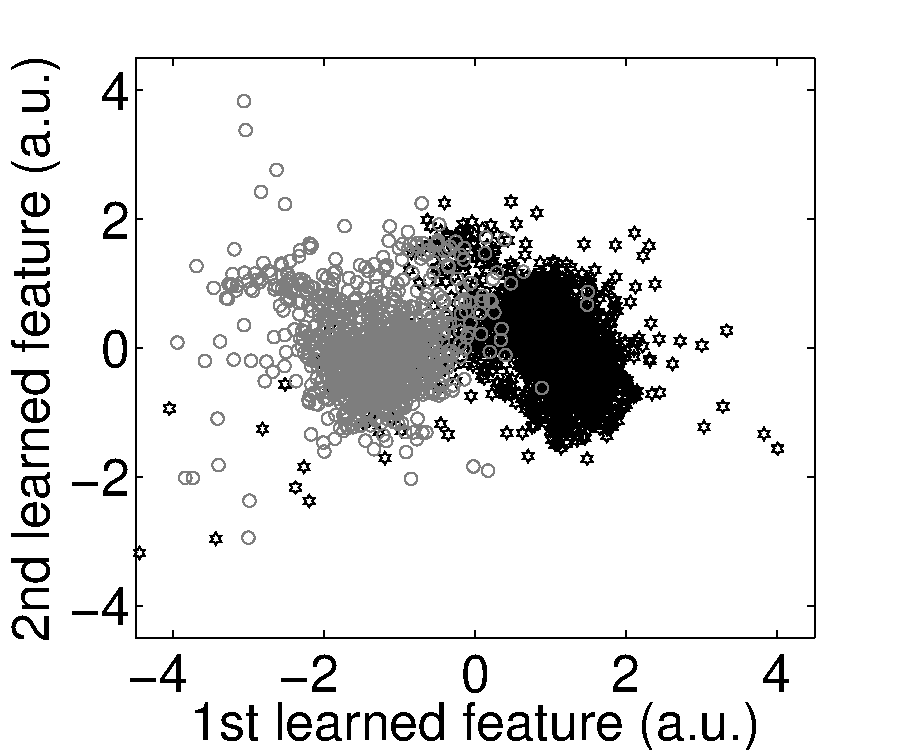
\includegraphics[scale=0.4,angle=0] {figs_new/Tuning_Parameter1.pdf}
   \label{fig:Tuning_Parameter1}
 }
 \subfigure[]{
   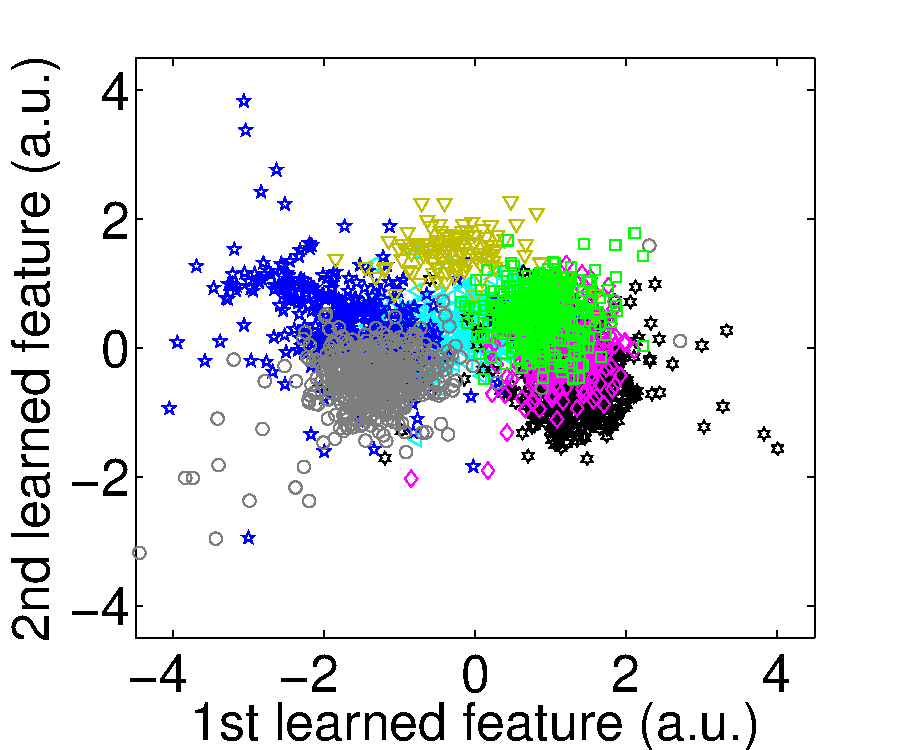
\includegraphics[scale=0.4,angle=0] {figs_new/Tuning_Parameter2.pdf}
   \label{fig:Tuning_Parameter2}
 }
  \caption{\label{fig:Tuning_Parameter}\small \emph{(a) Cluster results of feature spaces in the first two principle components with $\omega_0=10^{6}$, and the number of inferred clusters is two. (b) Cluster results of feature spaces in the first two principle components with $\omega_0=10^{8}$, and the number of inferred clusters is seven.
   }}
\end{figure}

\subsection{Computational requirements}

The software used for the tests in this paper were written in (non-optimized) Matlab, and therefore computational efficiency has not been a focus. The principal motivating focus of this study concerned forensics/interpretation of spike waveforms, as discussed in Section \ref{sec:forensics}, for which computation speed is desirable, but there is not a need for real-time processing ($e.g.$, for a prosthetic).
 Nevertheless, to give a sense of the computational load for the model, it takes about 20 seconds for each Gibbs sample, when considering analysis of 170800 spikes across $N=8$ channels; computations were performed on a PC, specifically a Lenevo T420 (CPU is Inter(R) Core (TM) i7 M620 with 4 GB RAM). Significant computational acceleration may be manifested by coding in C, and via development of online methods for Bayesian inference ($e.g.$, see \cite{Wang11}). In the context of such online Bayesian learning one typically employs approximate variational Bayes inference rather than Gibbs sampling, which typically manifests significant acceleration \cite{Wang11}.

\section{Conclusions\label{sec:conclusions}}

A new focused mixture model (FMM) has been developed, motivated by real-world studies with longitudinal ephys data, for which traditional methods like the hierarchical Dirichlet process have proven inadequate. In addition to performing ``focused'' clustering, the model jointly performs feature learning, via dictionary learning. The model explicitly models the count of signals within a recording period. The rate of neuron firing constitutes a primary information source \cite{Donoghue07}, and therefore it is desirable that it be modeled. This rate is controlled here by a parameter $p_i$, and this was allowed to be unique for each recording period $i$. In future research one may constitute a mixture model on $p_i$, with each mixture component reflective of a latent neural (firing) state; one may also explicitly model the time dependence of $p_i$. Inference of this state could be important for decoding neural signals and controlling external devices or muscles. In future work one may also wish to explicitly account for covariates associated with animal activity \cite{Ventura}, which may be linked to the firing rate we model here (we may regress $p_i$ to observed covariates).




\section*{Appendix}


\subsection{Proof of Lemma 3.1}

\begin{proof}
Denote $w_{j}= \sum_{l=1}^ju_{l}$, $j=1,\cdots,m$. Since $w_{j}$ is the summation of $j$ iid $\mbox{Log}(p)$ distributed random variables, the probability generating function of $w_{j}$ can be expressed as
$
G_{W_{j}}(z)=
\left[{\ln(1-pz)}/{\ln(1-p)}\right]^j,~ |z|<{p^{-1}}
$, thus we have
\beqs
& \mbox{Pr}(w_{j}=m) = {G_{W_{j}}^{(m)}(0)}/{m!} = \frac{d^{m}}{dz^{m}} [\ln(1-p z)/{\ln(1-p)}]^j \nonumber\\ &= (-1)^m p^j j! s(m,j)/[\ln(1-p)]^j \eeqs
%The detailed proof of this lemma can be found in Equations (22)-(26) of \cite{LGNB}. Here we use the property that
where we use the property that $[\ln(1+x)]^j = j!\sum_{n=j}^\infty\frac{s(n,j)x^n}{n!}$ \cite{johnson2005univariate}.
Therefore, we have
\beqs
%\mbox{Pr}(L = j|-) &\propto  \mbox{Pr}(w_{j}=m) \mbox{Pois}(j;-r\ln(1-p))
& \mbox{Pr}(\ell = j|-) \propto  \mbox{Pr}(w_{j}=n) \mbox{Pois}(j;-r\ln(1-p)) \nonumber\\ &\propto (-1)^{n+j}s(n,j)/n! r^j =F(n,j)r^j. \qedhere
%& = \frac{G_{W_{j}}^{(y)}(0)}{y!}  \mbox{Pois}(j;-r\ln(1-p))\nonumber\\
% = (-1)^{y+j}s(y,j)/y! r^j p^y\exp(r\ln (1-p))
%\label{eq:L_ik1} & = \left.\frac{d^{y}}{dz^{y}}f^j(z) \right| _{z=0} \frac{r^j }{j!y!} \exp(r\ln (1-p))\nonumber\\
%&=  F(y,j)r^j  p^{y}\exp(r\ln (1-p))
\eeqs
%Thus we have
%$ %\begin{align}
%%\label{eq:L_i_R}
%\mbox{Pr}(L = j|-) = R_r(y,j),~~j=0,\cdots, y
%%p(L_{i}|-)&\sim \delta(x_{i}>0)\mbox{Discrete} \left({R(x_{i},1) },\cdots,{R(x_{i},x_{i})  } \right). %,~~~\lambda_{ikj} = {F(x_{i},j) r^j  }
%$. %\end{align}
%and using (\ref{eq:L_ik1}) and (\ref{eq:R}),
%Note that to obtain (\ref{eq:L_ik1}), we use the relationship proved in Lemma 1 of the supplementary material %\ref{lem:H}
%that
%\begin{align} \label{eq:L_ik2}
%\left.\frac{1}{m!}\frac{d^{m}}{dz^{m}}f_i^j(z)\right|_{z=0} %& = \left. \sum_{j^\prime=1}^m H(m,j^\prime) \frac{j!}{(j-j^\prime)!}[f^{\prime}(z)]^{m}f^{j-j^\prime}(z) \right|_{z=0}\\
% &= F(m,j)j!p_i^{m},~~~ 1\le j \le m.
%\end{align}
\end{proof}
The values $F(n,j)$ can be iteratively calculated and each row sums to one, e.g.,
the 3rd to 5th rows are
\[ \left( \begin{array}{ccccccc}
2/3! & 3/3! & 1/3! & 0 & 0 & 0& \cdots \\
6/4! & 11/4! & 6/4! & 1/4! & 0 & 0& \cdots \\
24/5! & 50/5! & 35/5! & 10/5! & 1/5! & 0& \cdots \\
\end{array} \right).\]
To ensure numerical stability when $\phi>1$, we may also iteratively calculate the values of $R_\phi(n,j)$.



\subsection {Sparsely-firing problem}

\begin{figure*}[!htbp]
\centering

\subfigure[]{
   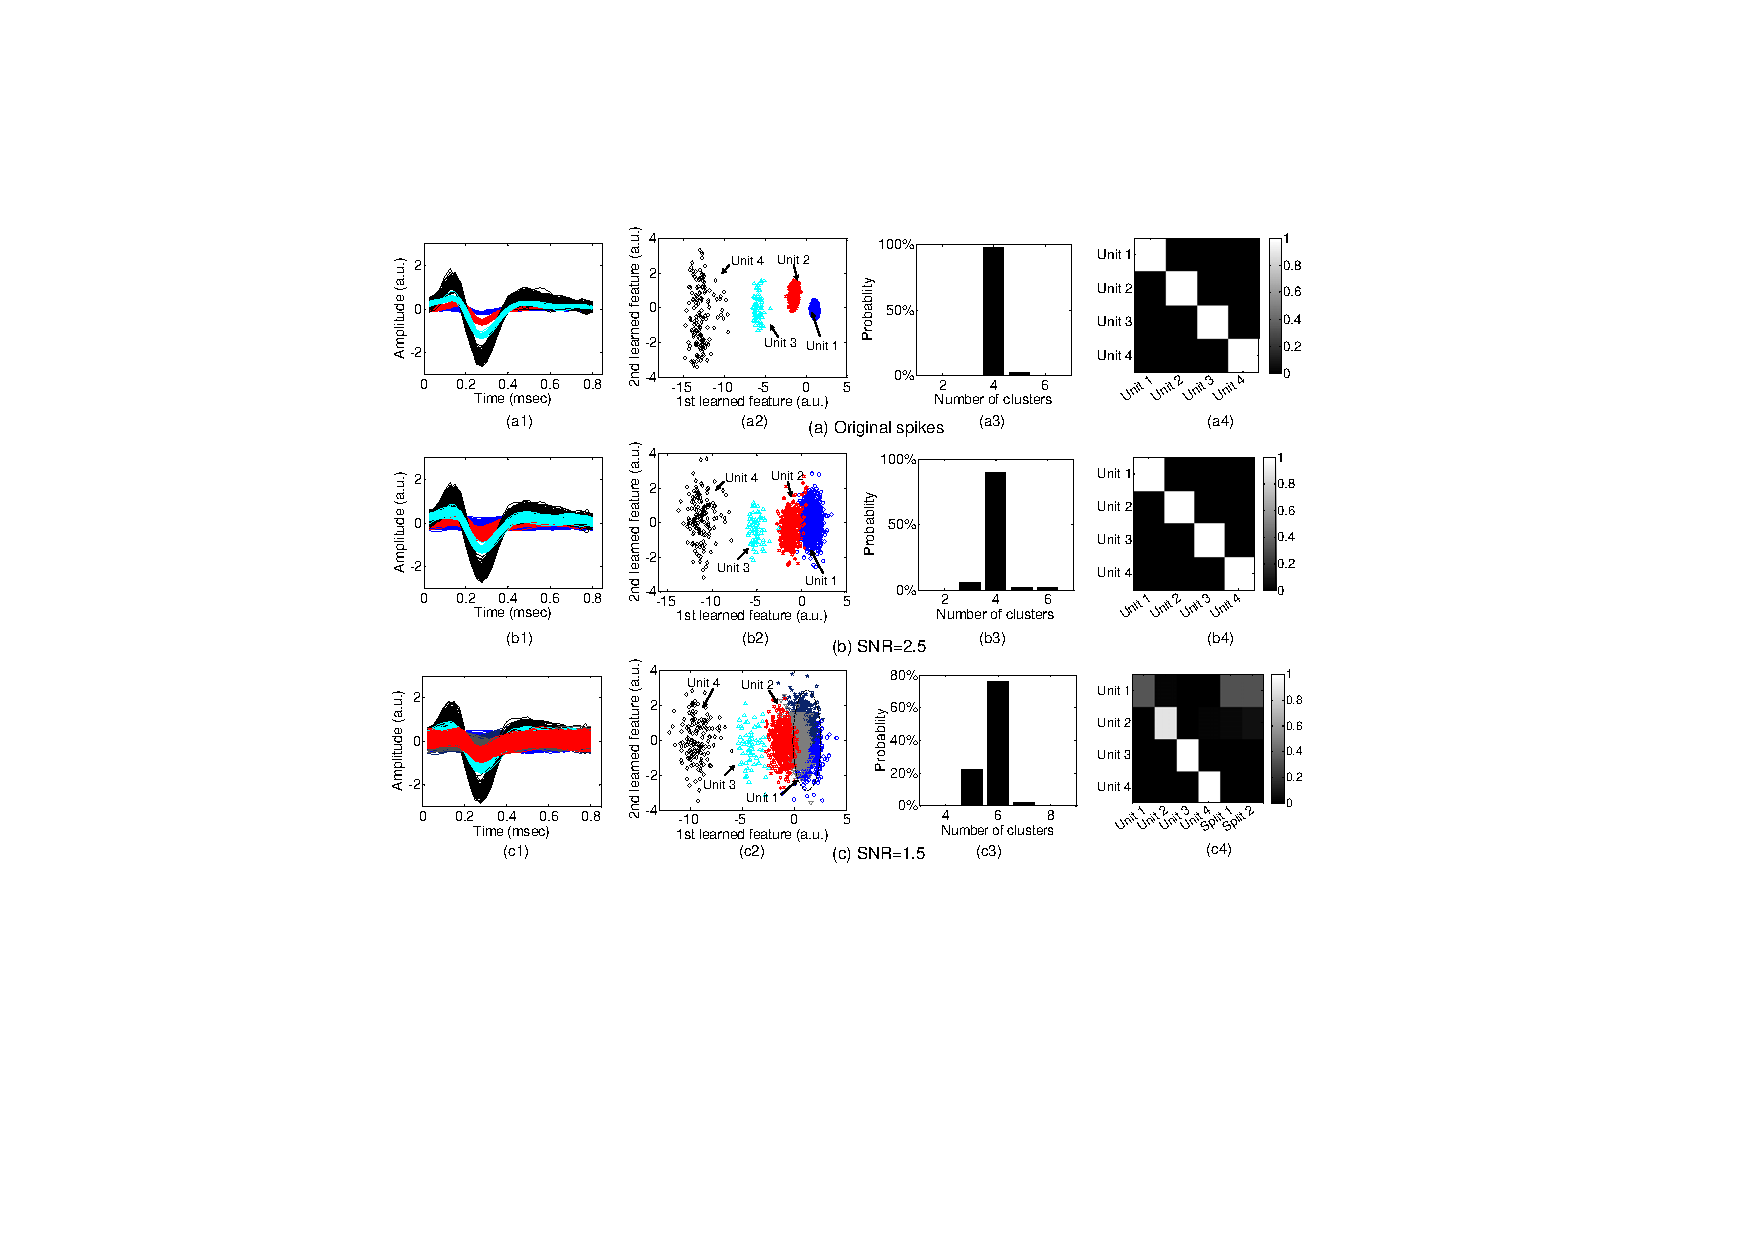
\includegraphics[scale=0.45,angle=0] {figs_new/sparse_firing.pdf}
   \label{fig:Sparse_firing_neuron}
 }
  \caption{}
\end{figure*}



\begin{figure}[!htbp]
\centering

 \subfigure[]{
   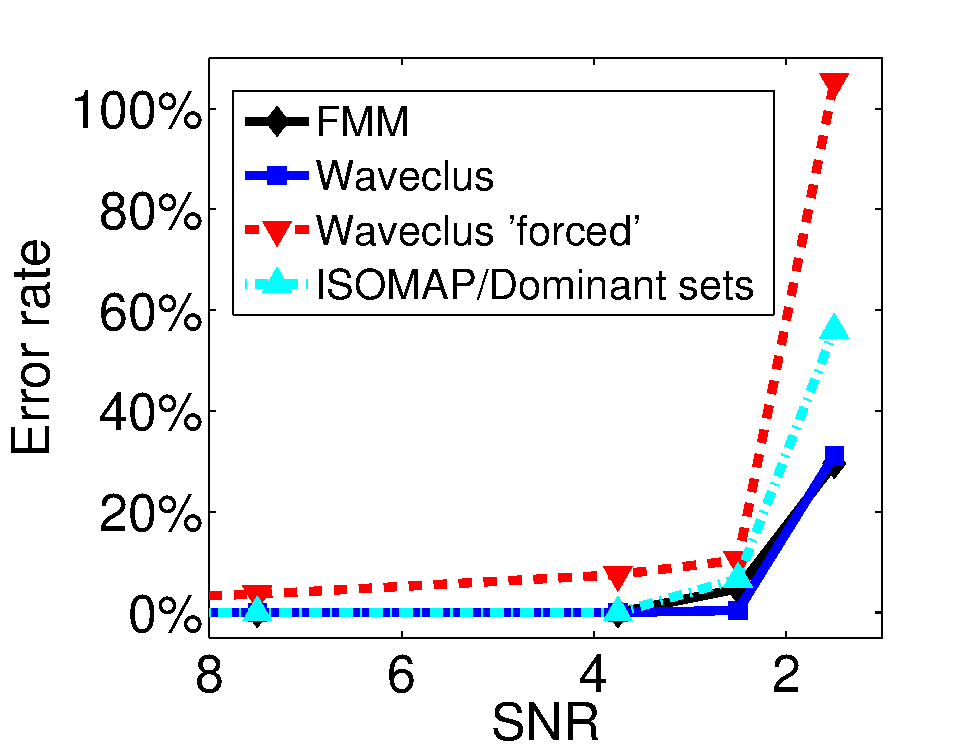
\includegraphics[scale=0.7,angle=0] {figs_new/error_rate.pdf}
   \label{fig:Terror_rate}
 }
 \subfigure[]{
   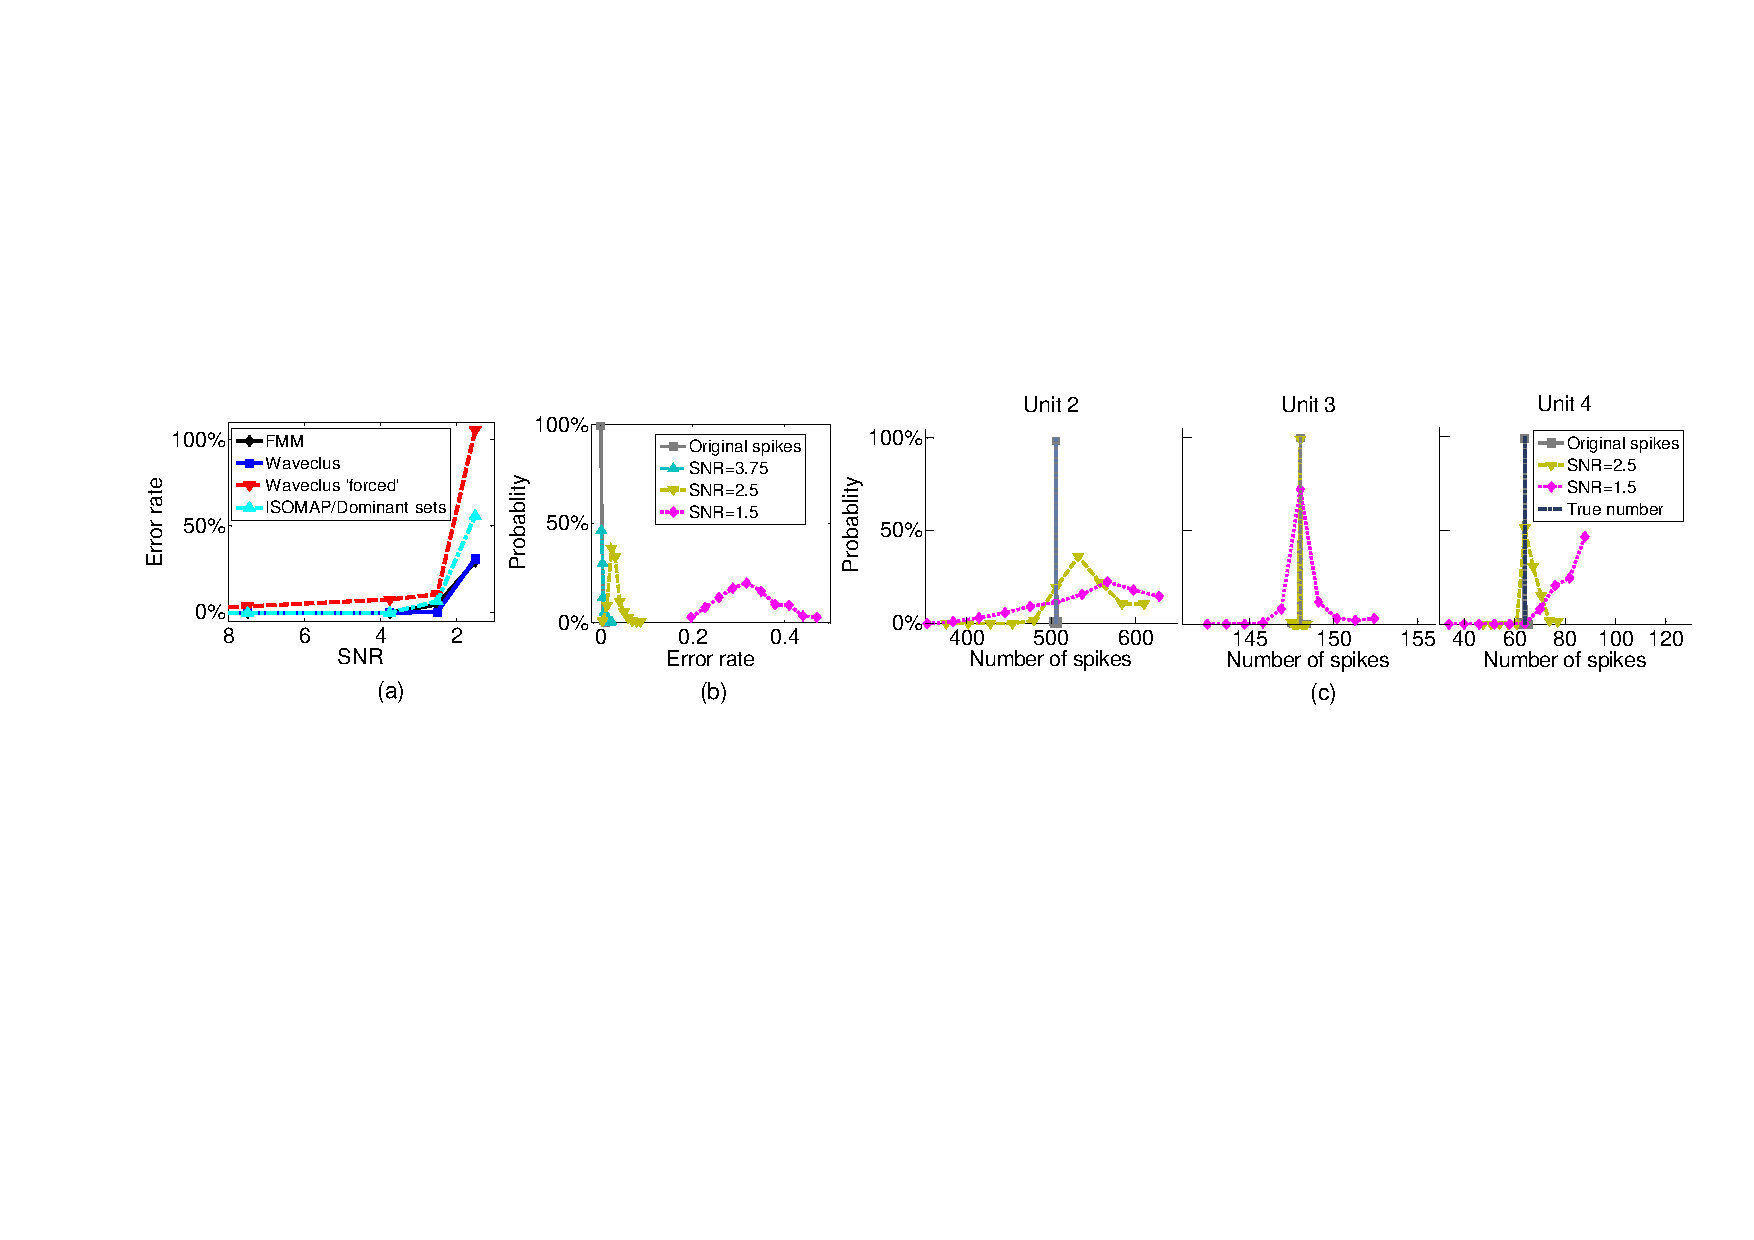
\includegraphics[scale=0.5,angle=0] {figs_new/posterior_error_rate.pdf}
   \label{fig:posterior_error_rate}
 }
  \caption{}
\end{figure}


\small\bibliography{PGFA_NIPS,myreference,Qisong_NIPS2012}%,,NIPS2012
\bibliographystyle{plain}


%\newpage
%
%the following figures are the distributions of  $p_i$,
%
%
%\vspace{-5mm}\begin{figure}[!htbp]
% \centering
%\subfigure[]{
%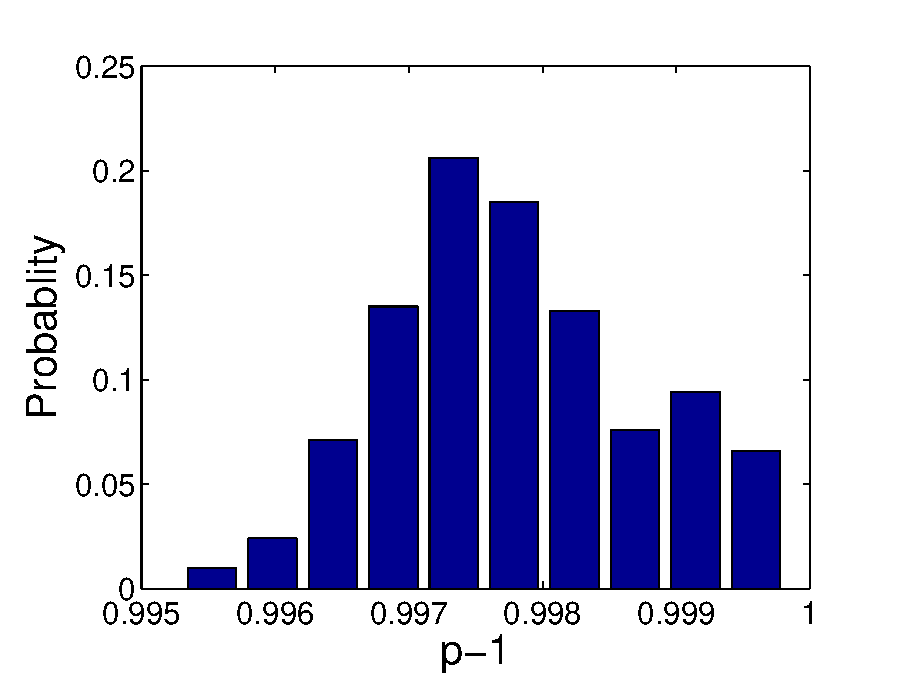
\includegraphics[scale=0.2,angle=0]{figs/Distribution_P_1.eps}
%\label{fig:P_1}}\vspace{-1.5mm}
%\subfigure[]{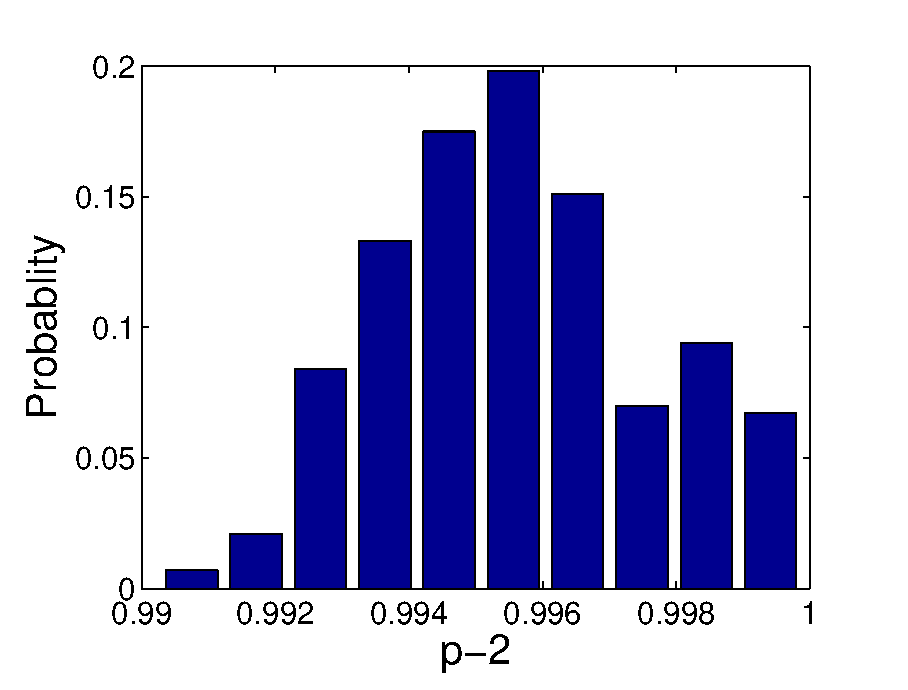
\includegraphics[scale=0.2,angle=0]{figs/Distribution_P_2.eps}
%\label{fig:P_2}}\vspace{-1.5mm} \subfigure[]{
%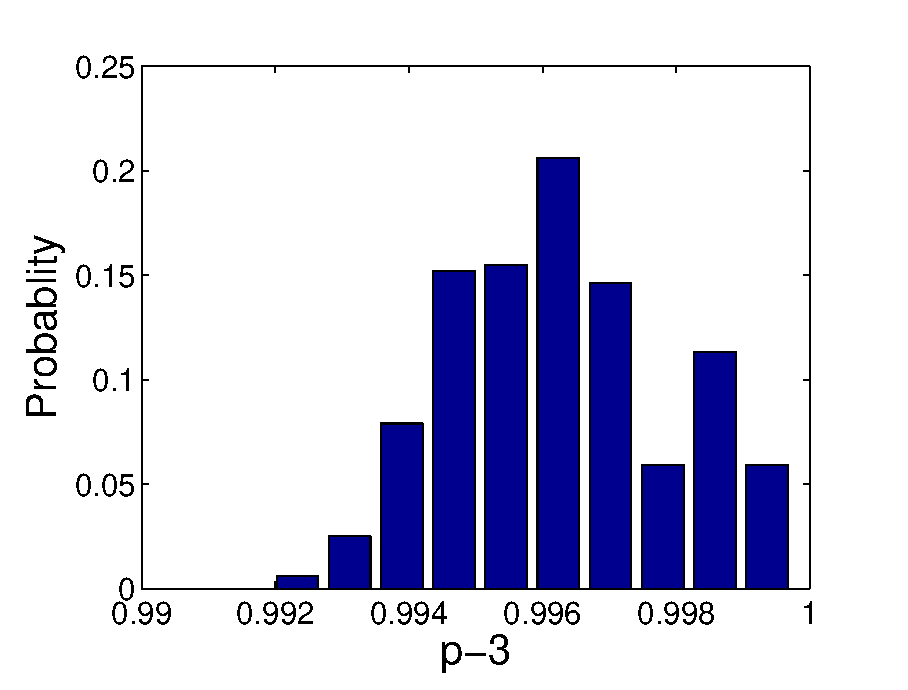
\includegraphics[scale=0.2,angle=0]{figs/Distribution_P_3.eps}
%\label{fig:P_3}}\vspace{-1.5mm}\subfigure[]{
%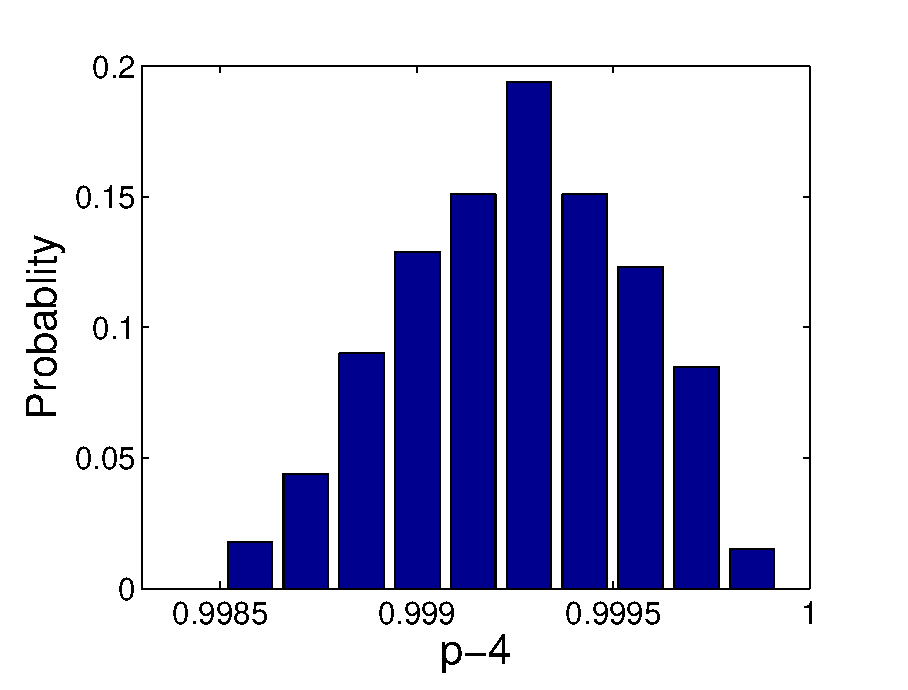
\includegraphics[scale=0.2,angle=0]{figs/Distribution_P_4.eps}
%\label{fig:P_4}}\vspace{-1.5mm}
%\subfigure[]{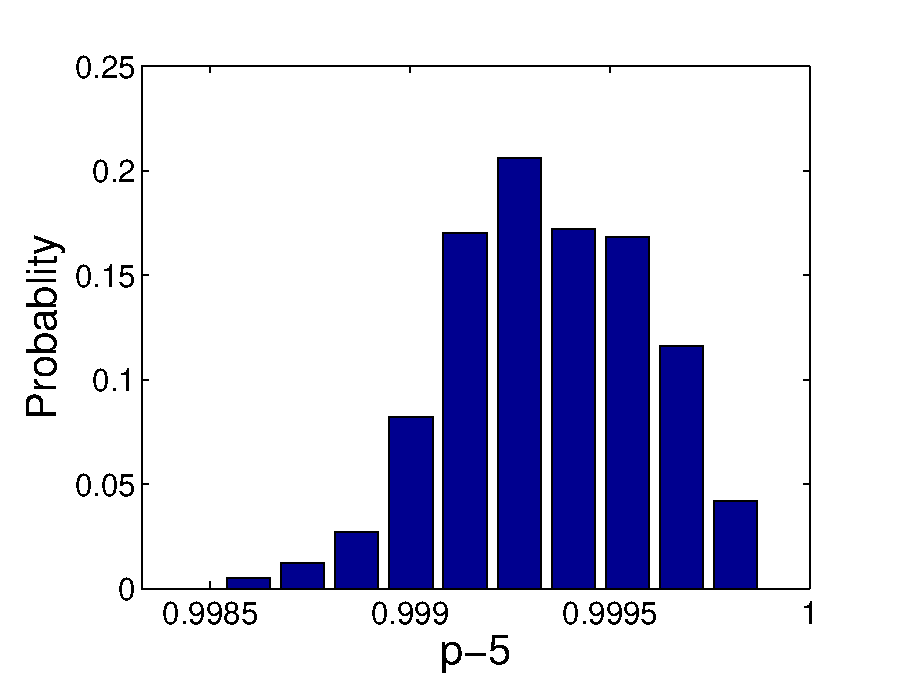
\includegraphics[scale=0.2,angle=0]{figs/Distribution_P_5.eps}
%\label{fig:P_5}}\vspace{-1.5mm} \subfigure[]{
%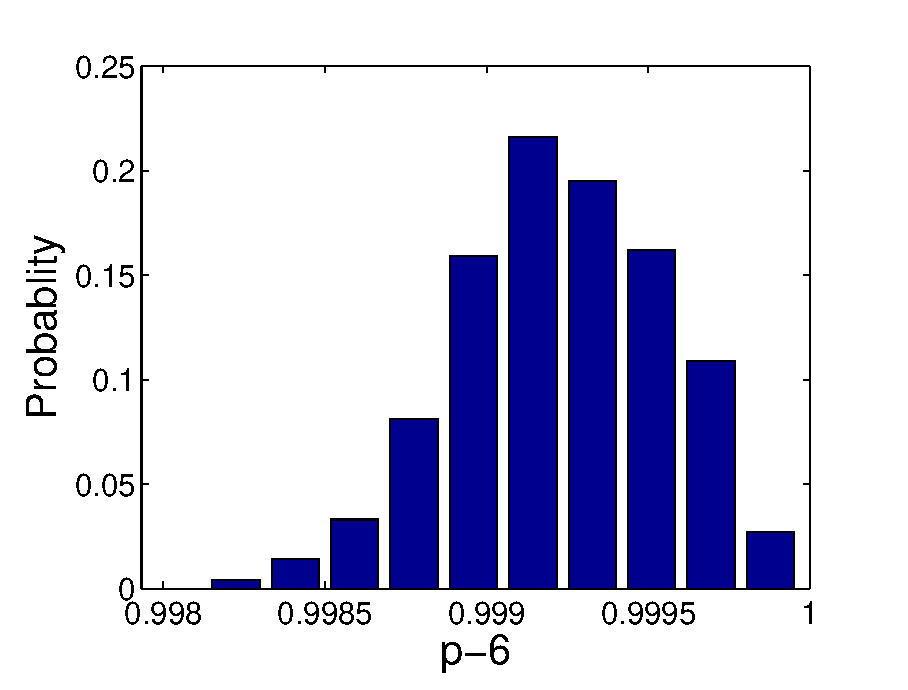
\includegraphics[scale=0.2,angle=0]{figs/Distribution_P_6.eps}
%\label{fig:P_6}}\vspace{-1.5mm}\subfigure[]{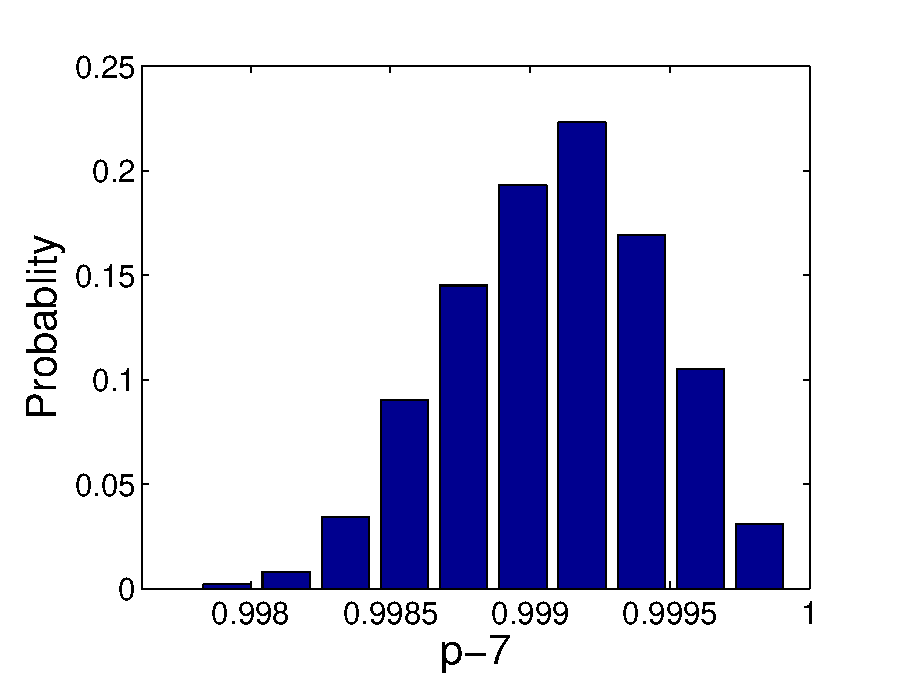
\includegraphics[scale=0.2,angle=0]{figs/Distribution_P_7.eps}
%\label{fig:P_7}}\vspace{-1.5mm} \subfigure[]{
%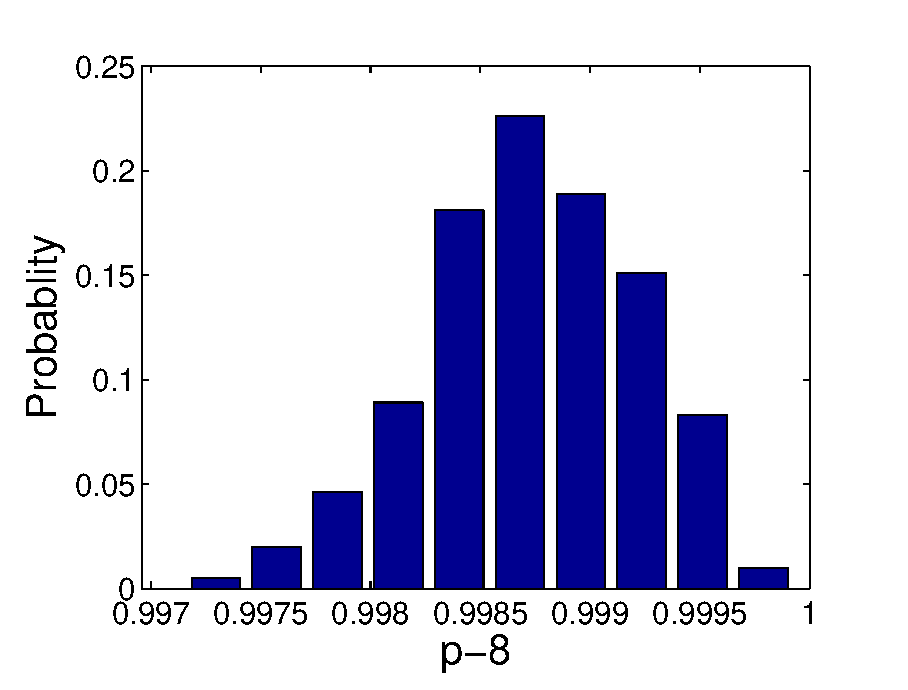
\includegraphics[scale=0.2,angle=0]{figs/Distribution_P_8.eps}
%\label{fig:P_8}} \vspace{-1.5mm}\caption{\label{fig:units}\small{}}
%\end{figure}\vspace{-10.0mm}





% that's all folks
\end{document}


